\documentclass[preprint,review,12pt,authoryear]{elsarticle}

\usepackage{amssymb}
\usepackage{amsmath}
\usepackage{latexsym}     
\usepackage{hyperref}
\usepackage{subcaption}
\usepackage{lineno}
\usepackage[margin=1in]{geometry}   

\usepackage{pstricks}
\usepackage{tikz} %required for wire diagram
\usetikzlibrary{shapes.geometric, arrows}
\usetikzlibrary{arrows,arrows.meta}
\usetikzlibrary{positioning} 
\usepackage{pst-node}
% add the following two lines to your document to get bigger arrows
\usetikzlibrary{arrows.meta}
\tikzset{>={Latex[width=3mm,length=3mm]}}

\def\ds{\displaystyle}

\journal{Ecological Modeling}

\begin{document}

\linenumbers
\begin{frontmatter}

\noindent {\bf This draft manuscript is distributed solely for purposes of scientific peer review. Its content is deliberative and predecisional, so it must not be disclosed or released by reviewers. Because the manuscript has not yet been approved for publication by the U.S. Geological Survey (USGS), it does not represent any official USGS finding or policy.} \\

\title{An integral projection model for gizzard shad (\emph{Dorosoma cepedianum}) utilizing density-dependent age-0 survival}

\author{ J. Peirce$^{\rm 1,3}$,  G.  Sandland$^{\rm 2,3}$, B. Bennie$^{\rm 1}$, R.A. Erickson$^{\rm 4}$}
\address{
${\rm 1}$ University of Wisconsin - La Crosse, Mathematics \& Statistics Department\\ 
${\rm 2}$ University of Wisconsin - La Crosse, Biology Department\\
${\rm 3}$ River Studies Center} 
${\rm 4}$ U.S. Geological Survey, Upper Mississippi Environmental Sciences Center\\ 

\begin{abstract}
%% Text of abstract
Gizzard shad (\emph{Dorosoma cepedianum}) is a common freshwater fish species found throughout the central and eastern portions of North America. 
Within these regions, gizzard shad play a number of critical roles in the freshwater community such as serving as prey for other fish species and translocating nutrients from substrates into the water column. 
Because of this, it is important that we understand how gizzard shad populations respond to environmental changes and what these changes may mean for aquatic communities in general and fish assemblages in particular. 
Here, we introduce an integral projection model (IPM) for gizzard shad that incorporates empirical information from a number of sources including Long Term Resource Monitoring (LTRM) data. 
IPMs are a generalization of stage-based, matrix population models that have been used to describe a wide range of organisms and, as such are a natural choice for gizzard shad since many aspects of their life cycle have been studied. 
We tested model outputs against empirical patterns reported for gizzard shad from a different location along the Illinois River (La Grange Reach). 
Results of our work suggest that our model could serve as an important tool for predicting gizzard shad population responses to changing environmental conditions, including those mediated through species invasions.
\end{abstract}

%%Graphical abstract
\begin{graphicalabstract}
\begin{figure}
    \begin{center}
%\scalebox{.75}[.75]{
\begin{tikzpicture}[->,>=stealth',shorten >=1pt,auto,node distance=3cm,
  thick,
  main node/.style={rectangle,draw},
  box/.style = {draw=gray, very thick,
                            minimum height=11mm, text width=11mm, 
                            align=center},]
                              
\node[main node, align=center] (census_pres) at (0,3) {Census $t$ \\
        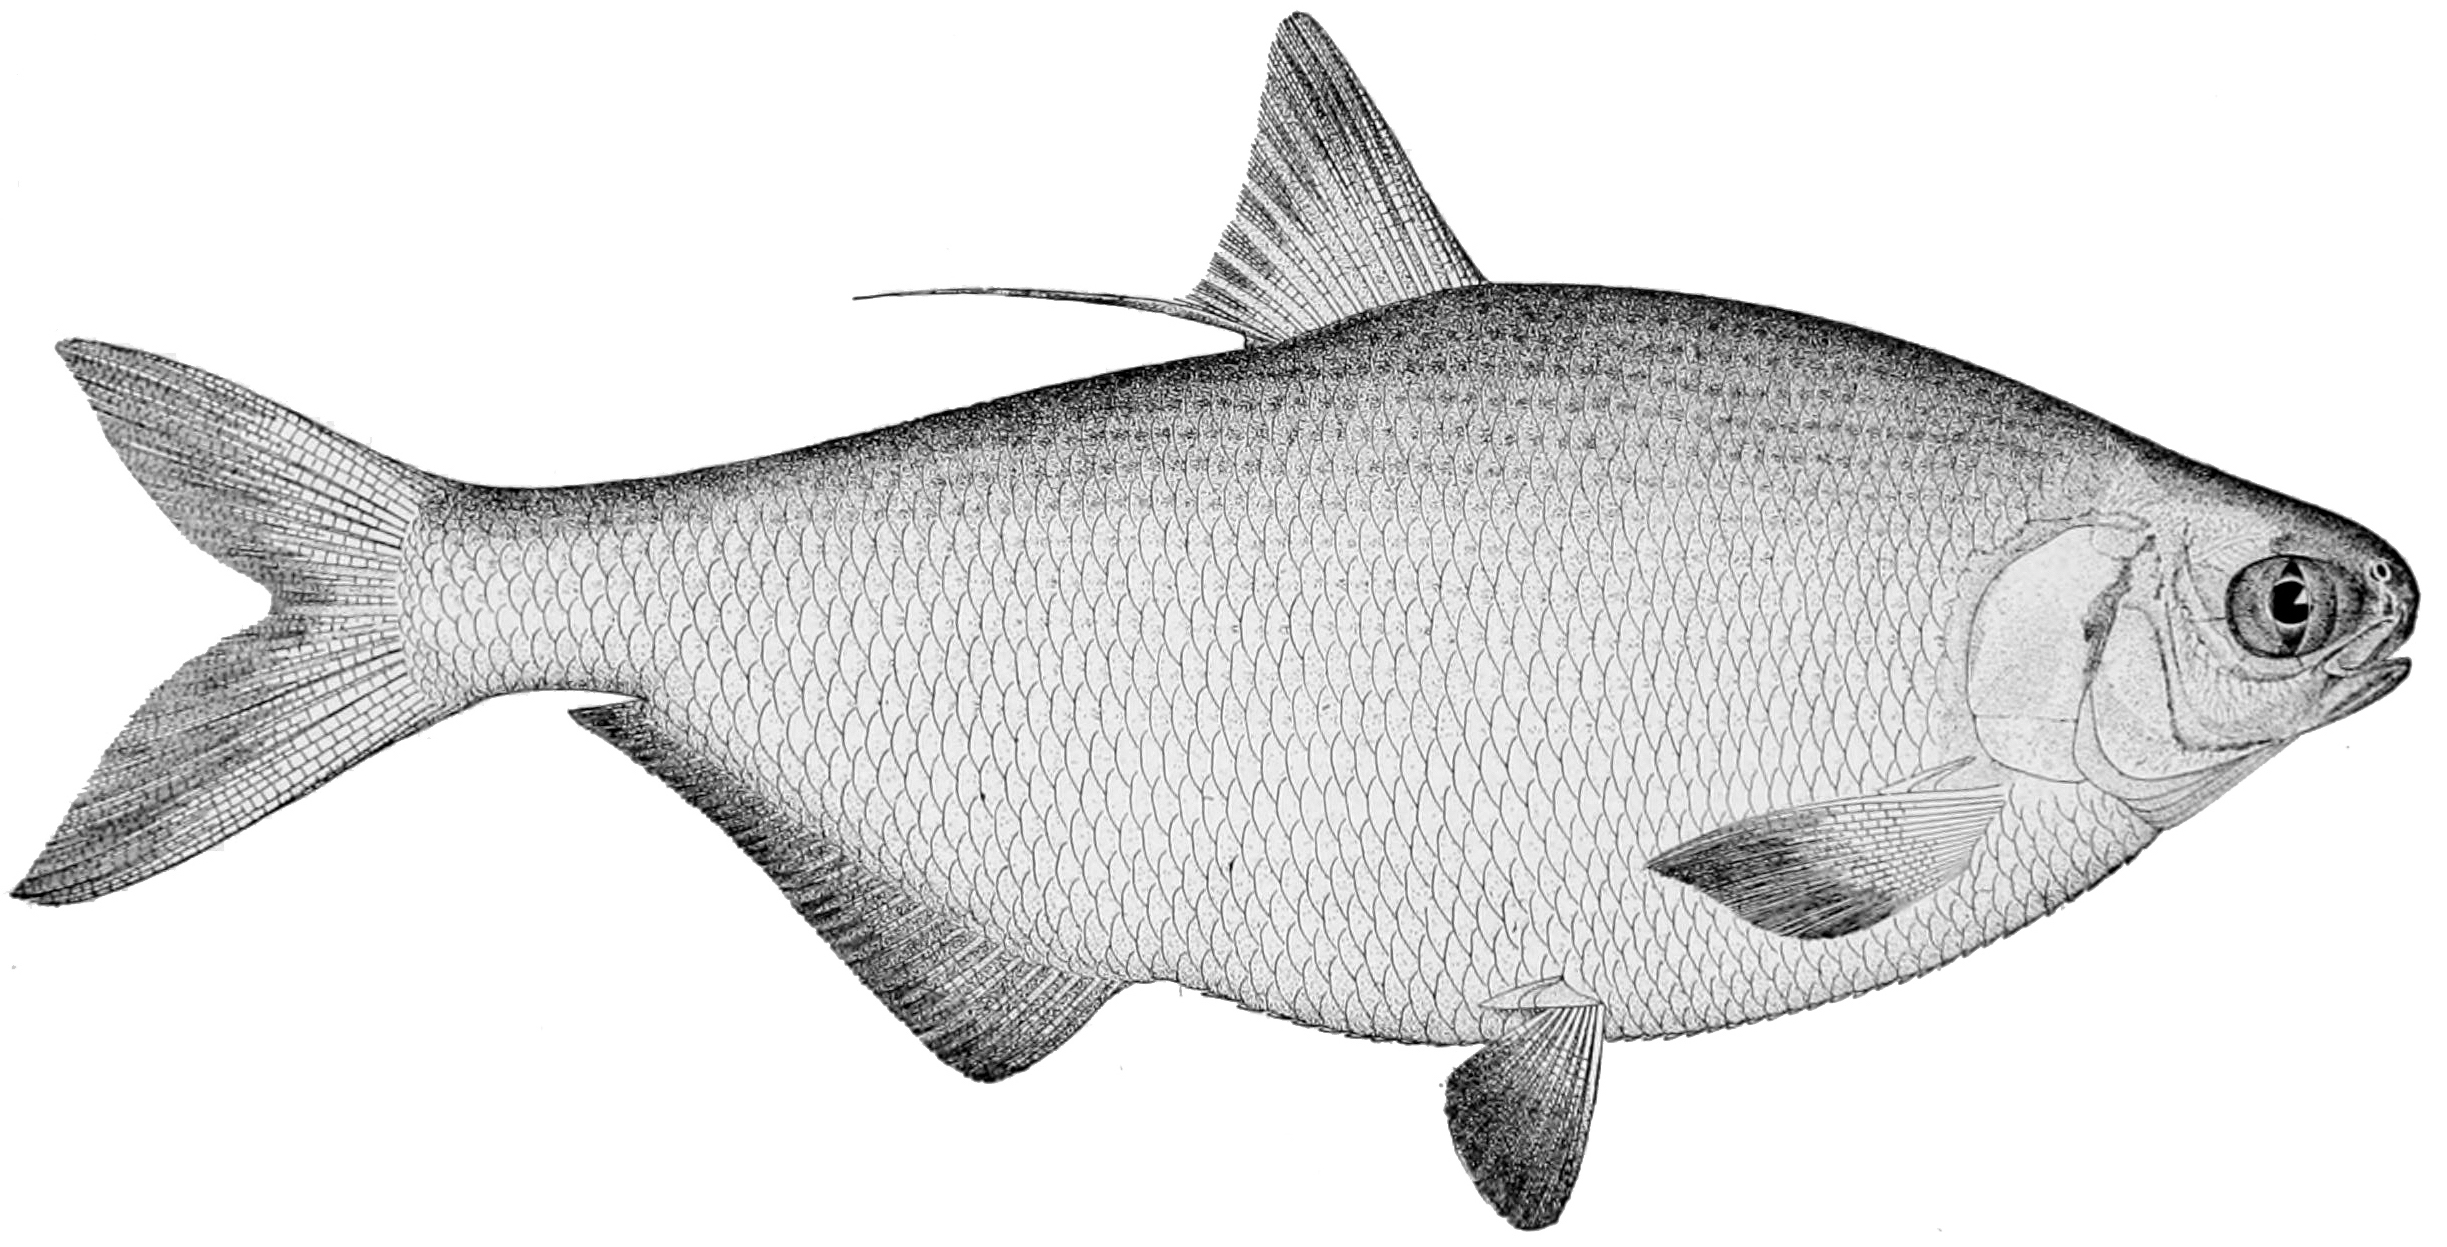
\includegraphics[width=0.12\textwidth]{adult.jpeg} \\
        $n(z,t)$};
\node[align=center] (repro) at (3.25,3) {Reproduction\\
        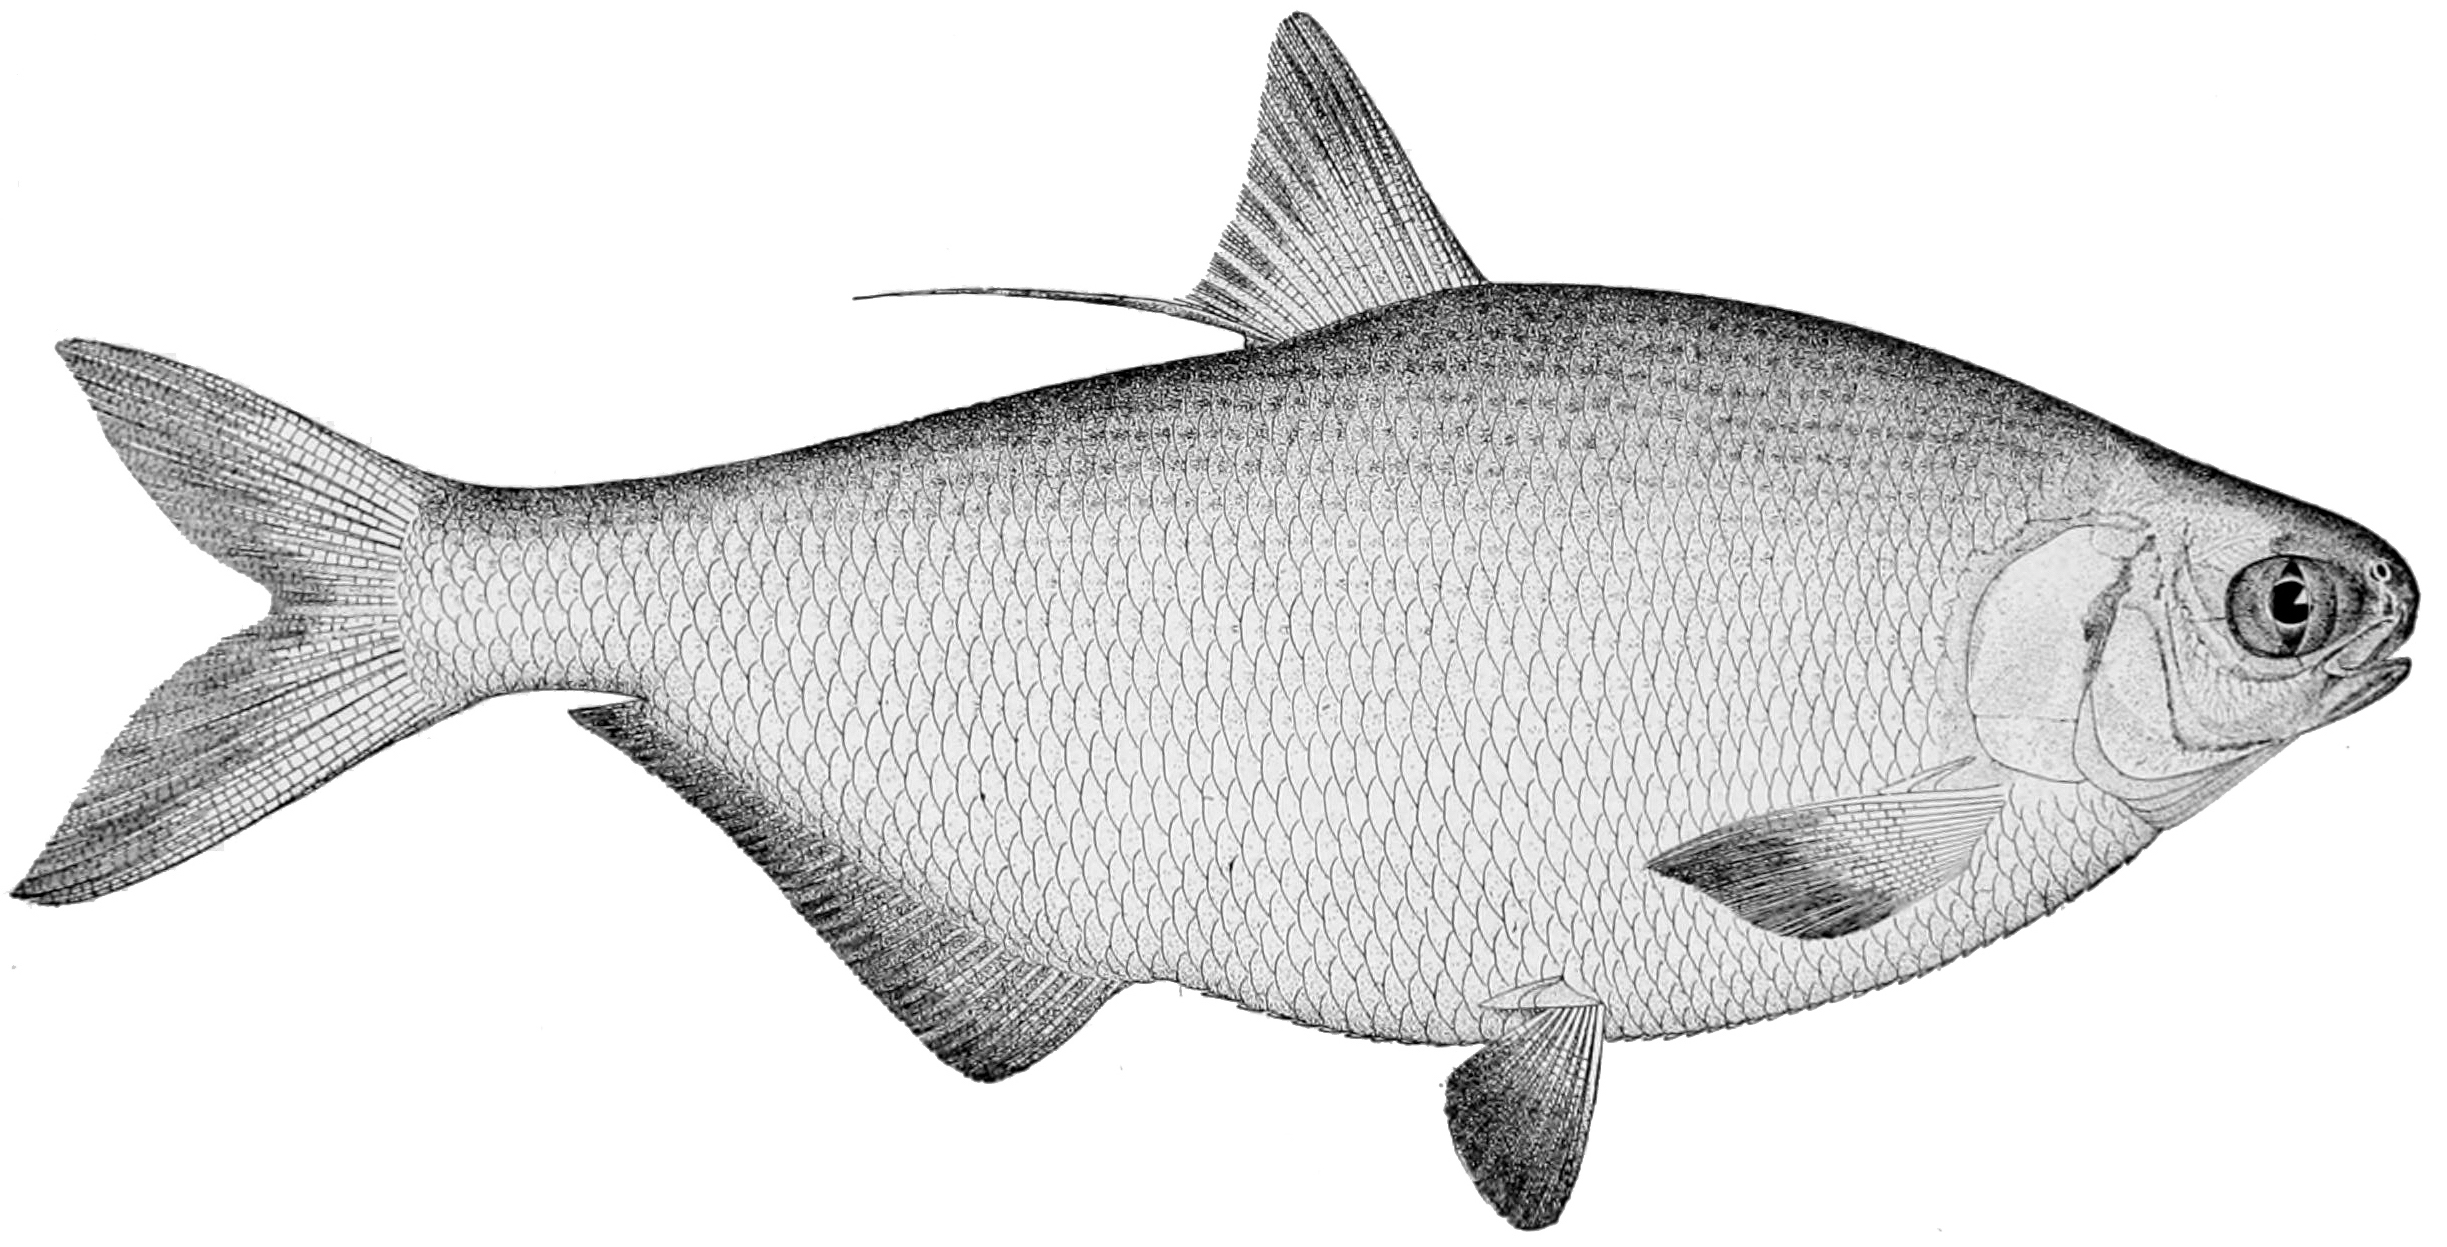
\includegraphics[width=0.12\textwidth]{adult.jpeg}\\
        };
\node (repro_in) at (2.3, 3)  {};
\node (repro_out) at (4.25, 3)  {};
\node (repro_down) at (3, 2.5)  {};
\node (grow_box) at (6.6,3.85) {Survival \& Growth};
\node[main node, align=center] (census_next) at (10,3) {Census $t+1$ \\
        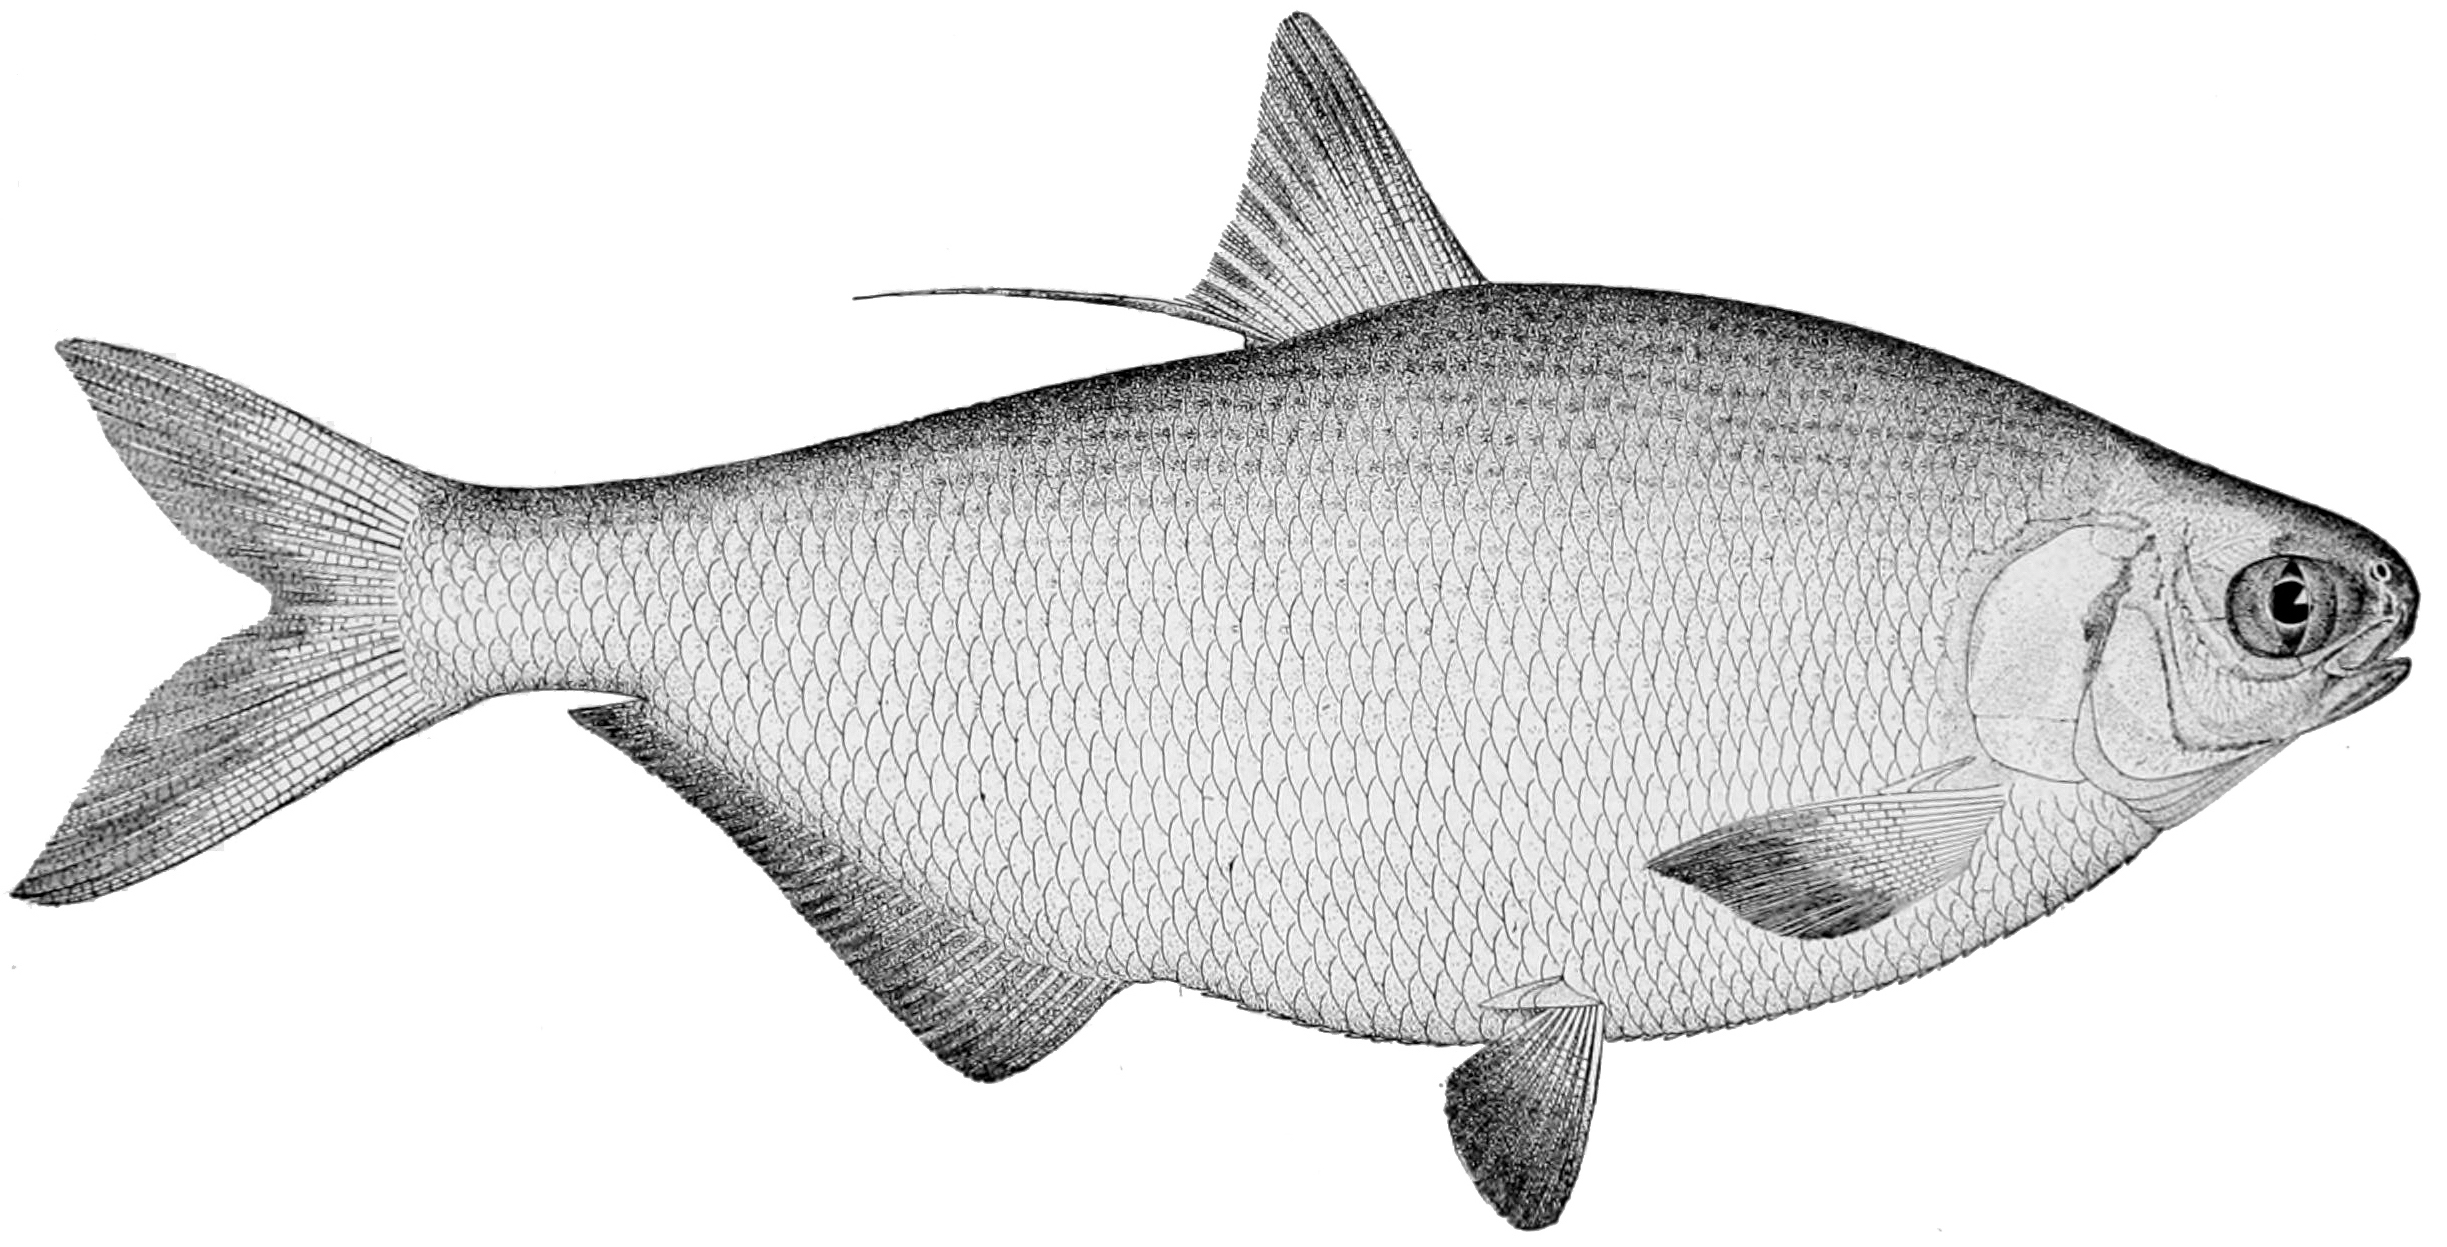
\includegraphics[width=0.15\textwidth]{adult.jpeg}\\
        $n(z',t+1)$};
\node (repro_box) at (13,3.85)  {Reproduction};
\node[align=center] (eggs) at (3,0) {Eggs \\ $\bullet$ $\bullet$ $\bullet$ $\bullet$ \\
  \, $\bullet$ $\bullet$ $\bullet$ $\bullet$ \\ $\bullet$ $\bullet$ $\bullet$ $\bullet$};
  \node[align=center] (eggs_viable) at (5,0) {Viable \\ $\bullet$ $\bullet$ $\bullet$ \\
  \, $\bullet$ $\bullet$ \\ $\bullet$ $\bullet$ $\bullet$};
 \node[align=center] (age1) at (8,0) { Age-1\\
        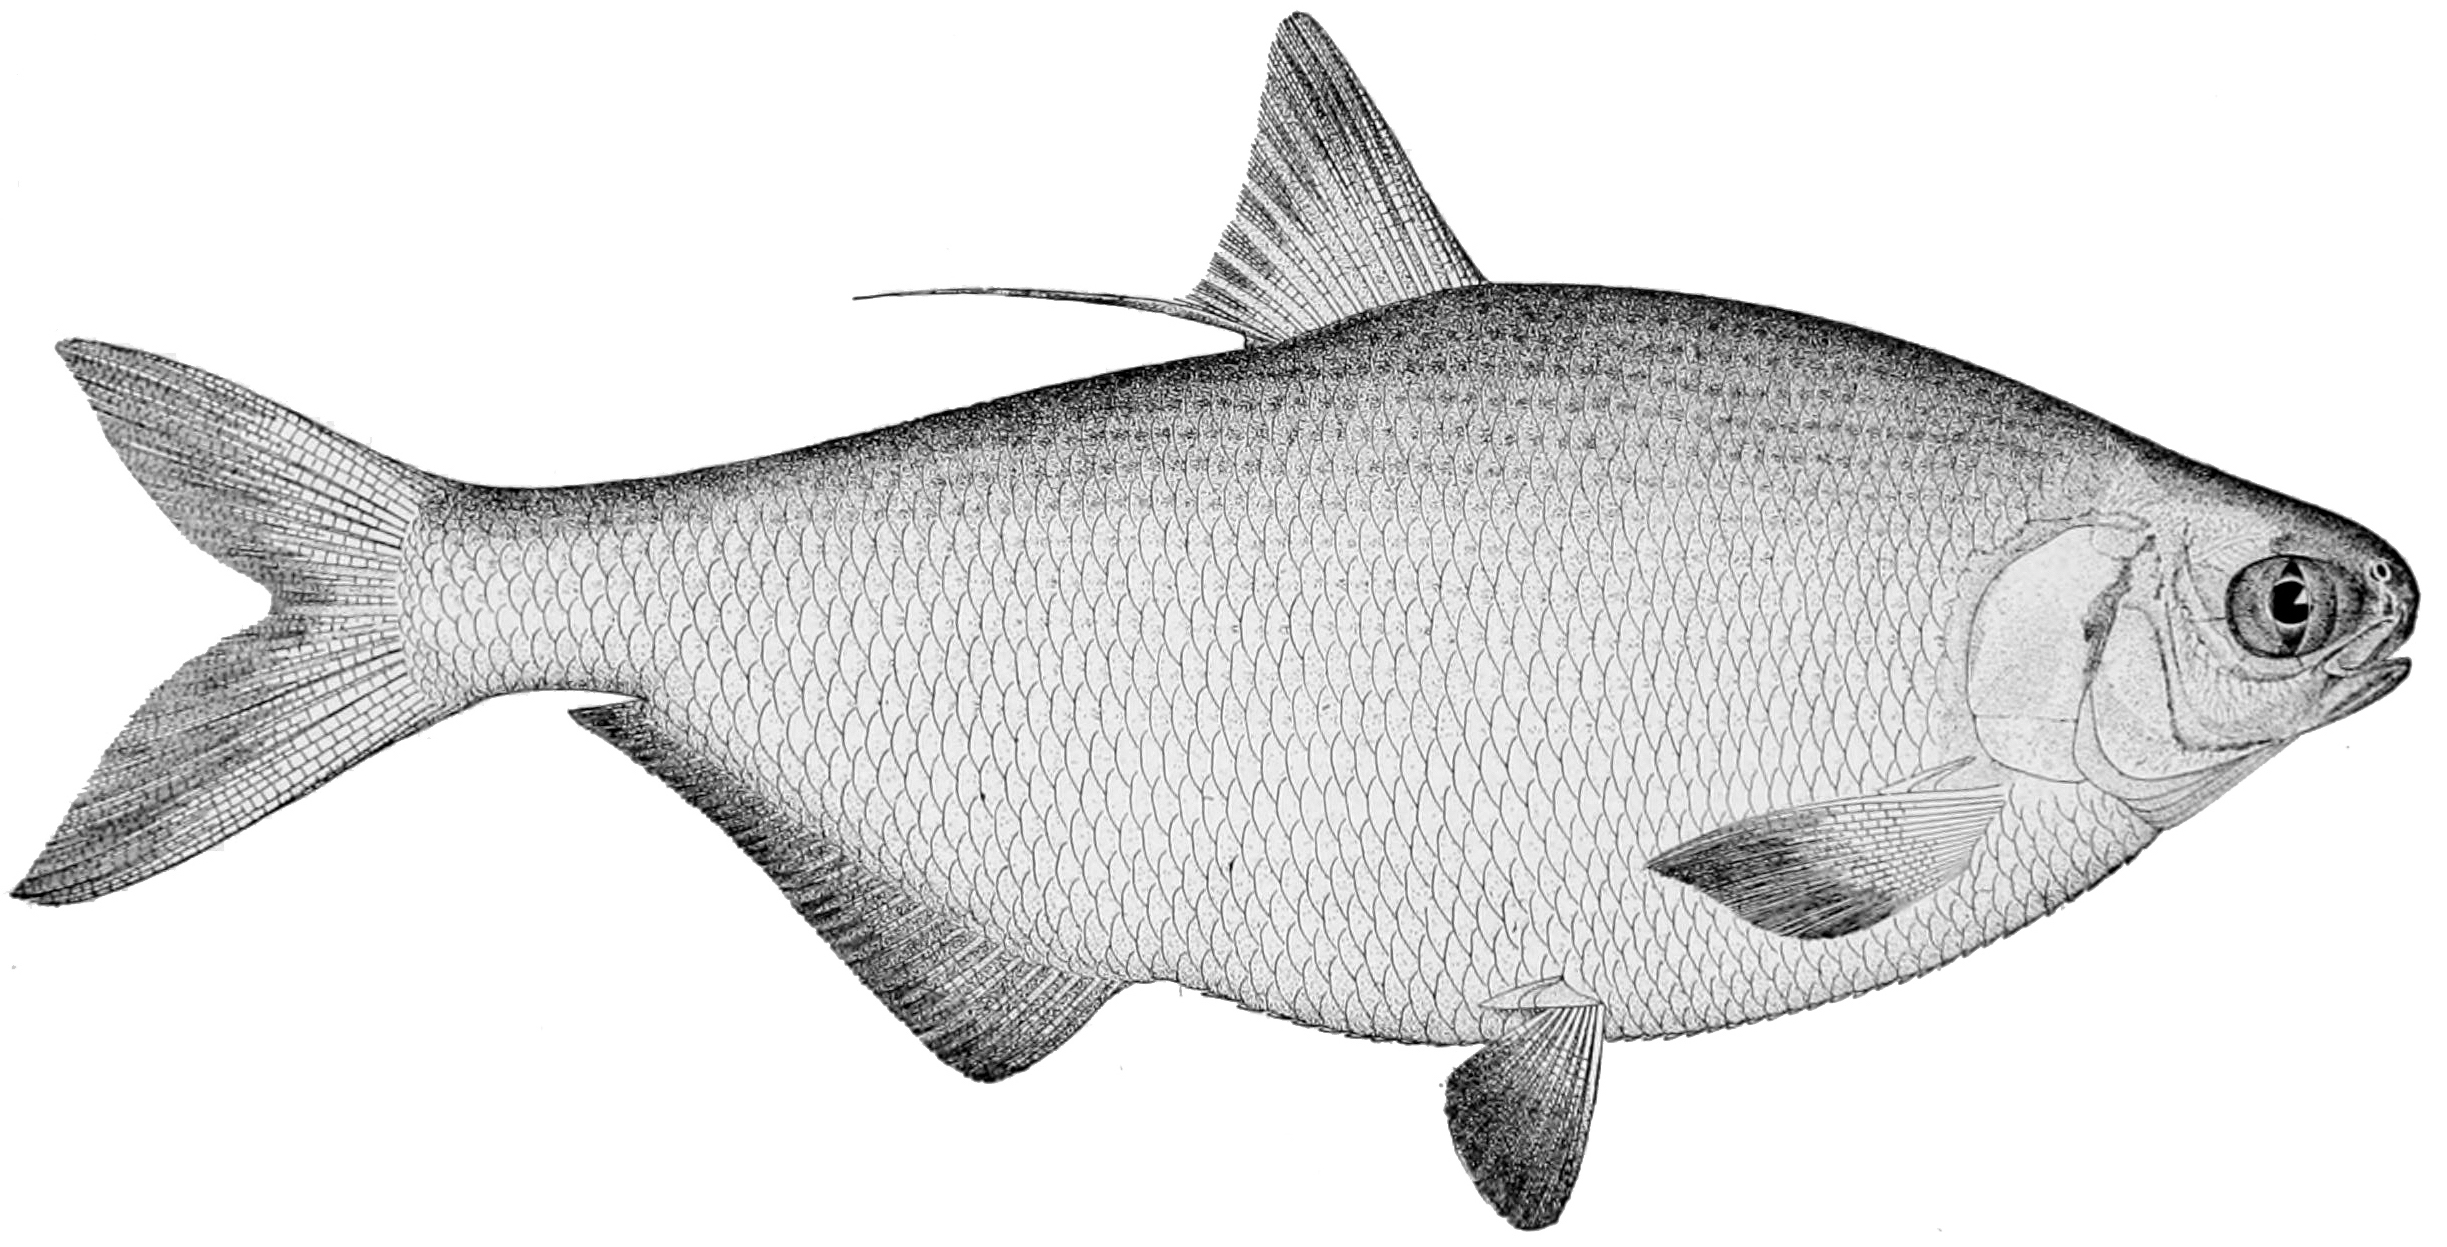
\includegraphics[width=0.06\textwidth]{adult.jpeg}
         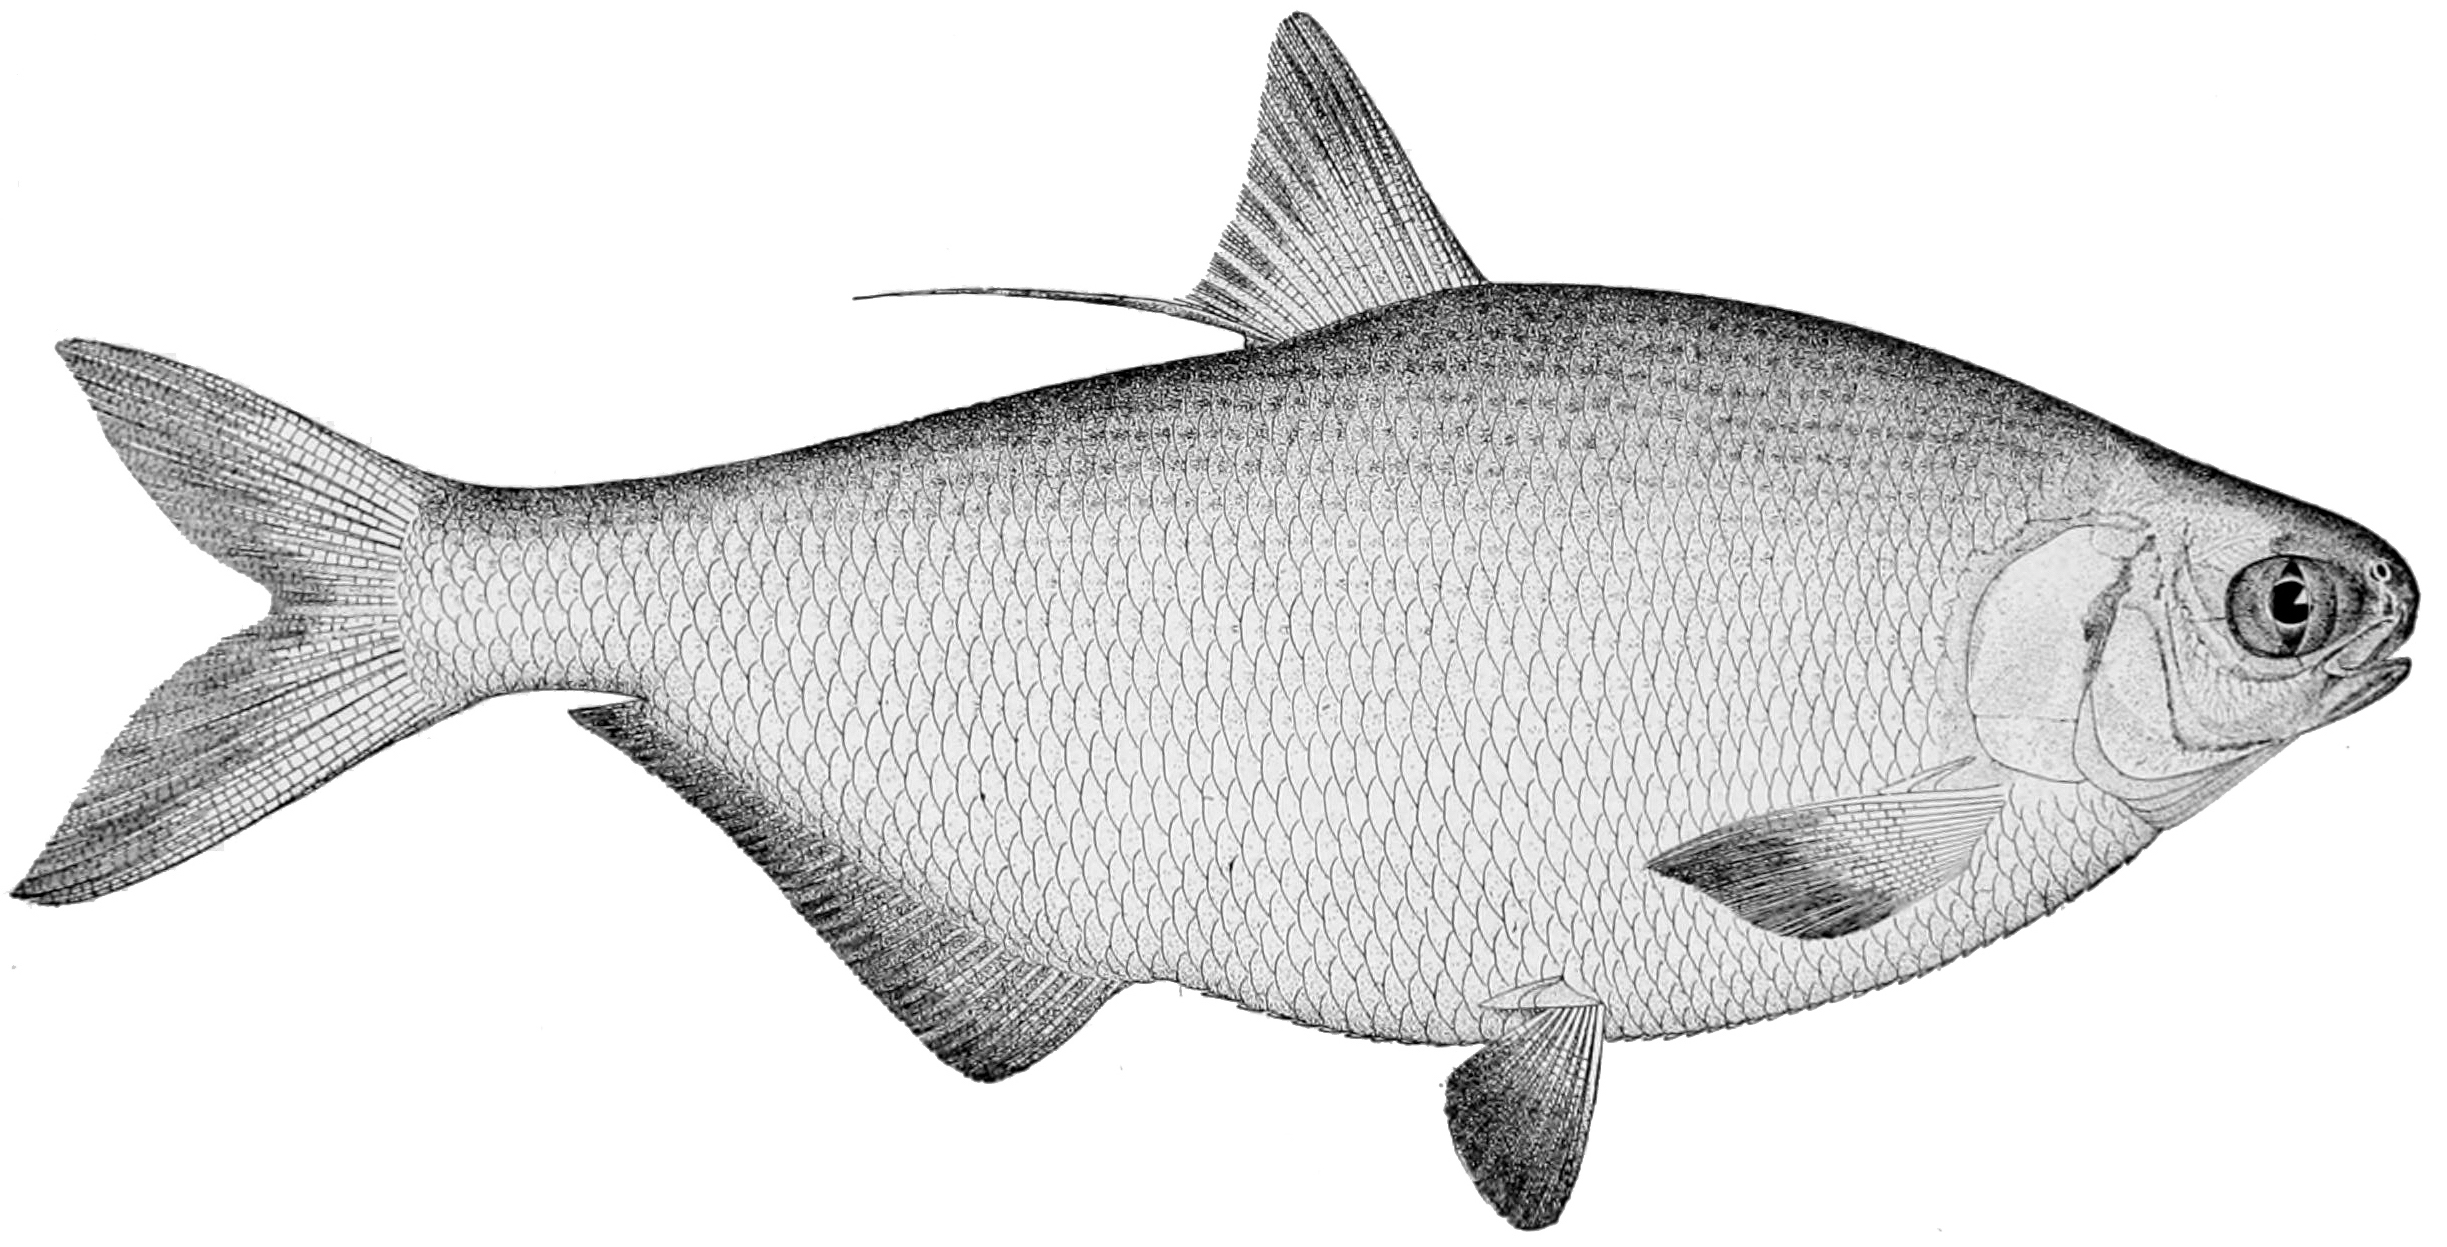
\includegraphics[width=0.04\textwidth]{adult.jpeg}\\
         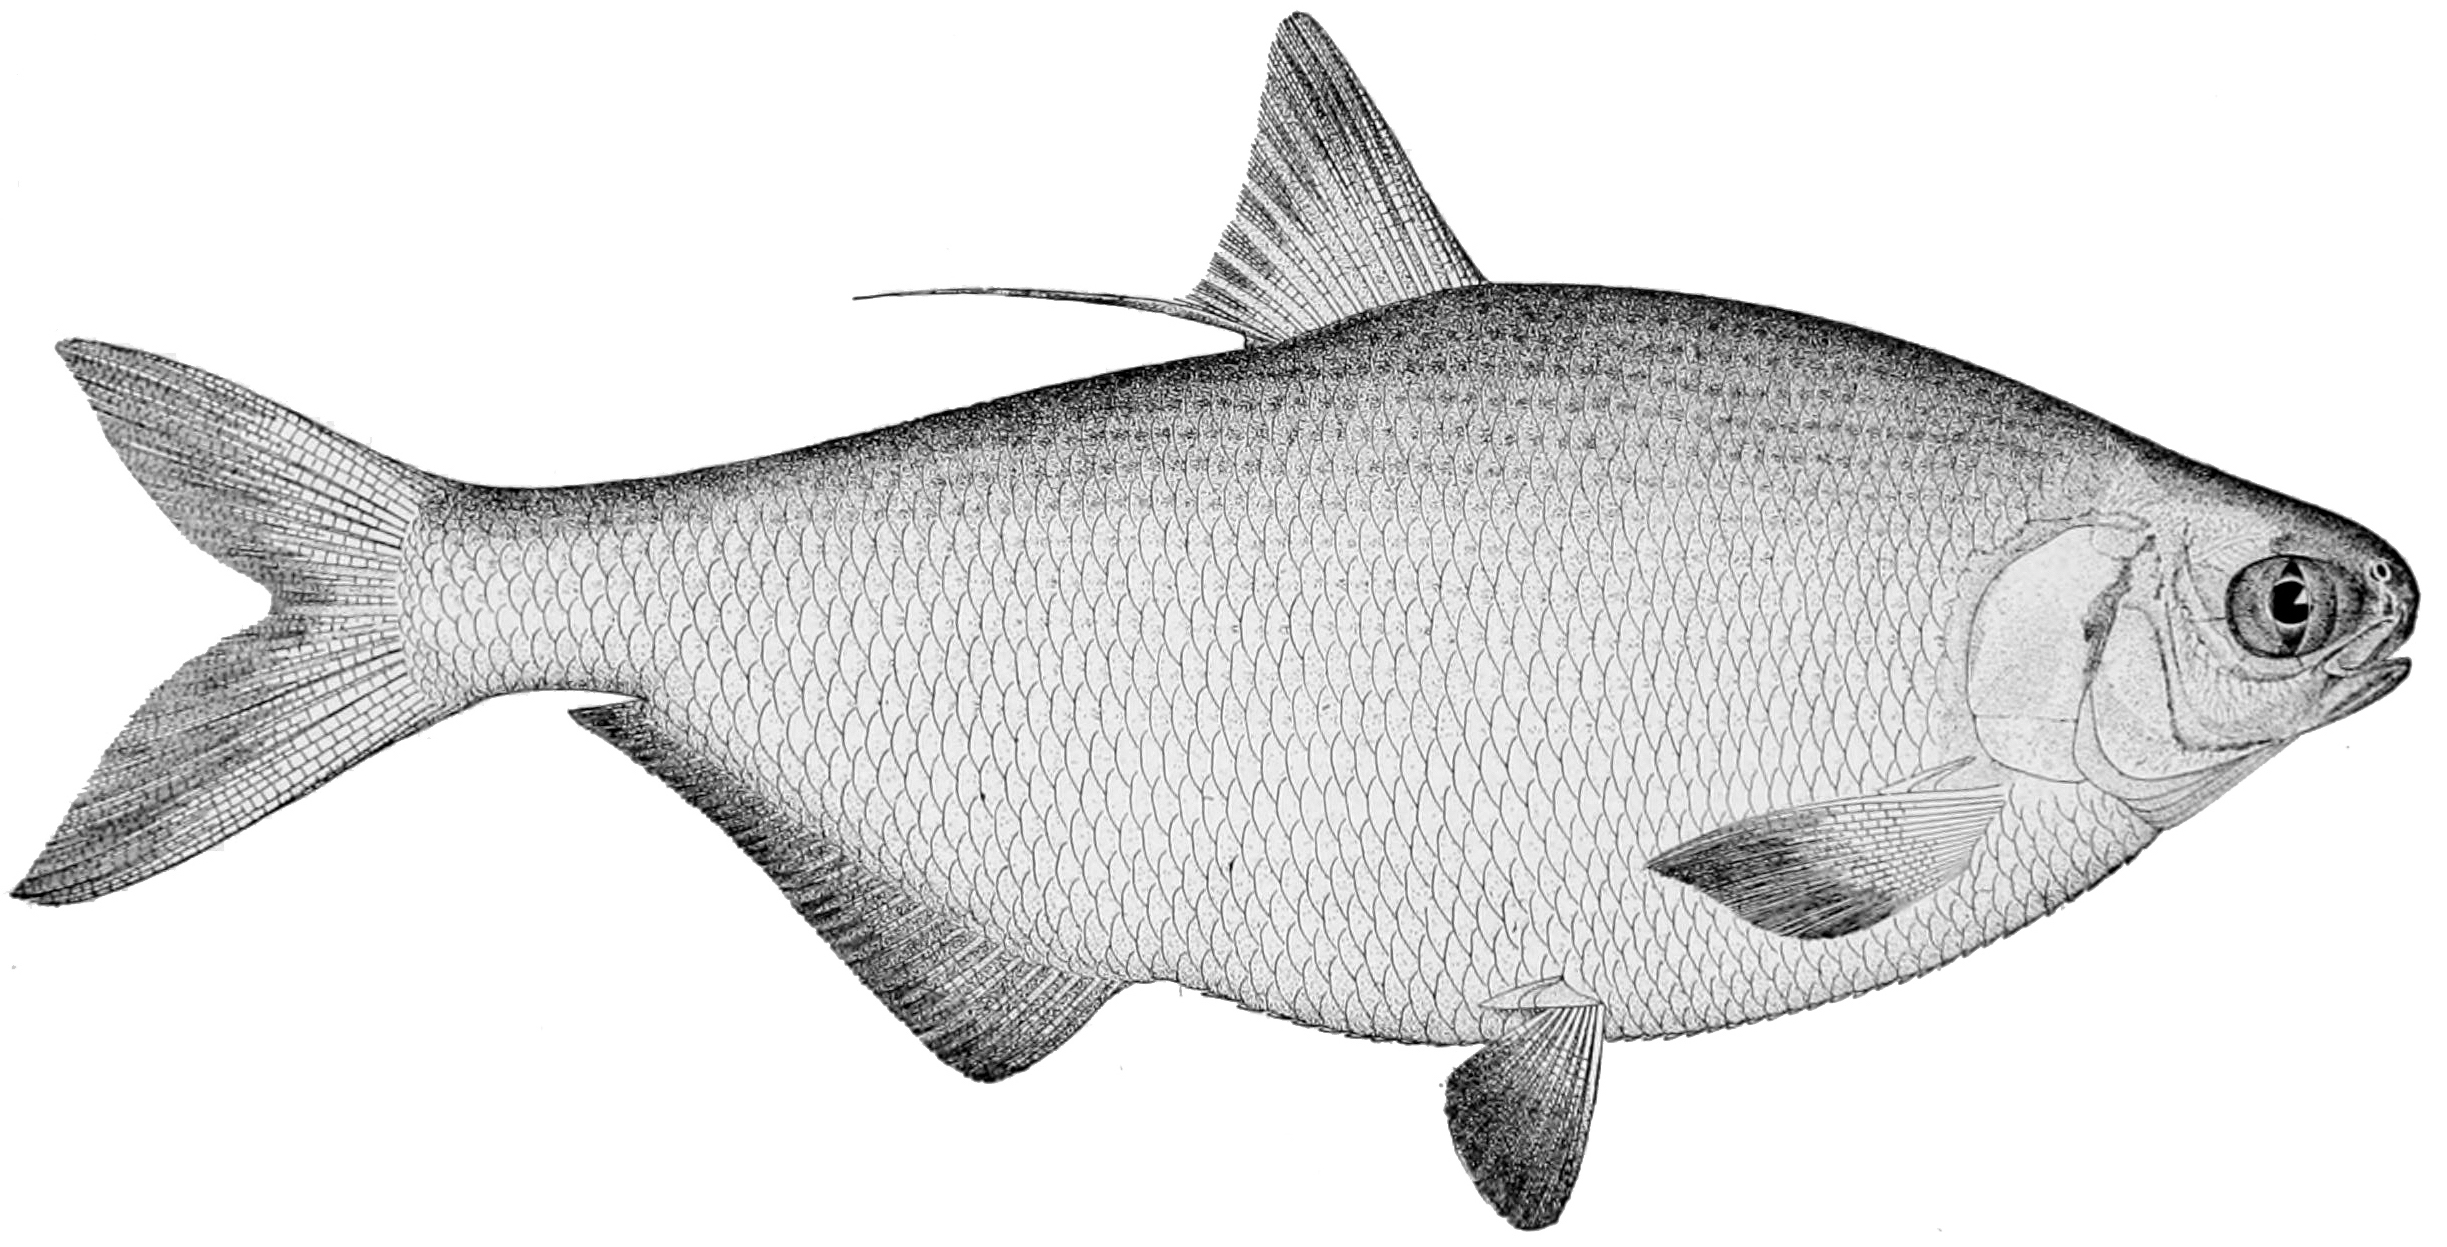
\includegraphics[width=0.08\textwidth]{adult.jpeg}
        };
\node[] (next) at (13,3) {};

\path[->]
	(census_pres) edge node {} (repro_in)
	(repro_out) edge node {$s(z)G(z',z)$} (census_next)
	(census_next) edge node {} (next)
	(repro_down) edge node {$p_b \rm{egg}(z)$} (eggs)
	(eggs) edge node {$\nu$} (eggs_viable)
	(eggs_viable) edge node {$s_0(d)$} (age1)
	(age1) edge node[right, pos=0.3] {$C_1(z')$} (census_next);
	
\end{tikzpicture}
%}
\end{center}
 \caption{\small{Life cycle diagram and census points for pre-reproduction census of gizzard shad used in a density-dependent integral projection model.}}
\end{figure}

\end{graphicalabstract}

%%Research highlights
\begin{highlights}
\item We introduce an integral projection model that incorporates data from studies on 1) egg production in different size classes of adult gizzard shad, 2) density-dependent survival of age-0 shad, and 3) length distributions of gizzard shad in the Upper Mississippi River system that span nearly thirty years.
\item  We establish survival parameters using gizzard shad data collected from the 5 sites along the Mississippi River and validate our model using empirical information collected from the La Grange Reach of the Illinois River.
\end{highlights}

\begin{keyword}
  population dynamics \sep
  fisheries \sep
  Mississippi River basin \sep
  population ecology \sep
  invasive species impact 

\end{keyword}

\end{frontmatter}

\section{Introduction}
Gizzard shad (\emph{Dorosoma cepedianum}) is a laterally compressed, deep-bodied fish species that occupies numerous aquatic systems throughout central, southern and eastern regions of the United States \citep{pierce1981aspects,vanni2005linking}.  
They have the potential to reach high abundances in more eutrophic habitats, such as reservoirs, leading to its dominance within fish assemblages. 
Because of this, gizzard shad have the potential to influence freshwater systems in a number of ways. 
First, young shad often serve as a critical food source for many fish species, including those of commercial and recreational importance (such as walleye and largemouth bass)\citep{jester1972life}. 
Thus, gizzard shad can serve as an important trophic link within aquatic food webs.
Second, because detritus can serve as a primary food source throughout much of gizzard shad development 
(i.e., from the age-0 stage onward), these fish can transport nutrients
from benthic regions into pelagic habitats \citep{mather1995regeneration, schaus2000effects, vanni2005linking}. 
This process can result in an increase in the nutrients available to organisms within the water column leading to increases in phytoplankton biomass, algal blooms, and, due to these conditions, shifts in freshwater community structure \citep{aday2003direct, schaus2000effects}. 
Finally, the fact that detritus can comprise a substantial portion of gizzard shad diet also makes this species an important connection between terrestrial inputs and aquatic processes \citep{schaus2000effects}.
Given its potentially important role in aquatic ecosystems, interest has intensified in understanding how gizzard shad populations respond to environmental changes (both natural and anthropogenic) and what these changes may mean for freshwater communities in general and fish assemblages in particular.

Interactions within and between species throughout interconnected environments can have important consequences for fish populations across space and time \citep{thorp2006riverine}.  
For gizzard shad, previous work has suggested that fish densities can play an important role in both the growth and survival patterns observed in populations of these fish.  
For example, \citep{buynak1992differential} reported an inverse relationship between densities and the lengths of age-0 gizzard shad.  Similarly \citep{welker1994growth} found that high densities of age-0 shad were negatively associated with both fish length and survival under both field and semi-natural conditions. Finally, \citep{michaletz2010overwinter} reported that the densities of age-0 gizzard shad were negatively correlated with survival in two Missouri lakes.  
These patterns were attributed to intraspecific competition among young shad for prey (zooplankton) resources. Although intraspecific competition may be influencing life-history traits in subsequent stages of gizzard shad development, little work has actually been conducted to address this \citep{dicenzo1996relations}. 
There is also evidence that the densities of other co-occurring fish species (such as invasive carps) may negatively influence aspects of gizzard shad biology, such as body condition \citep{irons2007reduced,love2018does}.

Although substantial empirical work on gizzard shad biology has accumulated over the decades, few if any studies have attempted to use these data to model population dynamics in this species.
Work by \citet{catalano2010size, catalano2011whole} used empirically-based simulations of gizzard shad to assess population-level responses in this species.
As part of this process, the authors investigated population-structure using fish lengths but did
not consider the impacts of gizzard-shad densities on population patterns.
Here, we introduce an integral projection model (IPM) for gizzard shad based on empirical data with density-dependent survival in age-0 fish.
We then compare model outcomes to the dynamics reported for this fish species in a well-studied pool of the Illinois River (specifically, the La Grange Reach).
Results from this work suggest that our model could be an important tool for predicting gizzard shad population responses to changing environmental conditions, including those mediated through species invasions (i.e., silver and bighead carp).

\begin{table*}
  \caption{A summary of parameters, their biological meaning, and source for mean values.
  }
 \begin{center}
	\resizebox{\textwidth}{!}{
\begin{tabular}{p{6.5cm}|p{6cm}|c| p{6cm}  }\hline
     Parameter & Meaning (units) & Mean& Source \\\hline
Logistic survival probability function, $s(z)$ & & \\
  $\ds s_{\rm {min}}$ & minimum survival & 0.002 & \citep{bodola1955life} \\
  $\ds s_{\rm {max}}$ & maximum survival & $\ds 1-8.871K^{0.73}L_{\infty}^{-0.33}$ 
  & THEN 2015 \\ 
 $\ds \alpha_s$  & inflection point & 80.01 & Estimated from LTRM dataset \\
  $\ds \beta_s$ & slope & -139.93 & Estimated from LTRM dataset \\\hline
  Growth function, $\ds G(z,z')$ & & \\
  $L_\infty$ & maximum length (in mm) & 394.30 & \citep{catalano2010size} \\
  $K_g$ & individual growth rate & 0.26 &  \citep{michaletz2017variation} \\
  $\sigma_g$ & growth standard deviation & 25 &  \citep{michaletz2017variation} \\\hline
  Normal distribution of length of age-1, $\ds C_1(z')$ & & \\
  $\mu_r$ & mean length of recruitment (in mm) & 105 & \citep{michaletz2017variation} \\
  $\sigma_r$  & standard deviation of length & 25 & \citep{michaletz2017variation} \\\hline
Eggs produced, egg(z) & & \\
$\ds \mbox{egg}_{\mbox{max}}$ & maximum number of eggs produced & 737512.1 & Estimated from \citep{jons1997ovarian} \\
$\ds \alpha_e$ & inflection point & 314.44 & Estimated from \citep{jons1997ovarian} \\
$\ds \beta_e$ & slope & -7.18 & Estimated from \citep{jons1997ovarian} \\\hline
Survival of age-0, $s_0(d(t))$ & & \\
$\ds a_0$ & intercept & 0.27 & Estimated from \citep{michaletz2010overwinter} \\
$\ds b_0$ & decay rate & 0.003 & Estimated from \citep{michaletz2010overwinter} \\\hline
Spawning & & \\ 
 $\nu$  & probability that egg becomes viable & 0.002 & \citep{bodola1955life} \\
 $p_b$ & probability that female spawns & 0.90 &    \\ 
 \end{tabular} } \label{table:parameters}
     \end{center}
     \end{table*}    

\section{Model development}
\subsection{Gizzard shad life history}
Mature gizzard shad tend to mate between May and June, although this can vary based on water temperatures. 
Males and females aggregate and then broadcast gametes into the surrounding water; fertilized eggs then settle and adhere to the bottom substrates. 
After a period of days, eggs hatch and fish develop from the larval stage to juveniles and eventually to adults. 
In many habitats, individuals can reach sexual maturity within a year. 
As gizzard shad mature, their diet preferences typically shift from phytoplankton and zooplankton early in development to detritus and zooplankton as adults. 
Given the large number of eggs produced by shad females ($>$ 300,000/year), there is evidence that intraspecific competition can be intense during early developmental stages in this species leading to density-dependent mortality. 
The strength of competition may then subside as fish transition to feeding on different food types during later stages of development.   

\subsection{Equations}
We used an IPM to describe the life history of gizzard shad in the Upper Mississippi River system (UMRS). 
IPMs were first introduced by Easterling \citep{easterling2000size}, as a generalization of stage-based, matrix population models. 
Since that time, IPMs have been used to describe a wide range of organisms \citep{ellner2016data, merow2014advancing, rees2014building}, but have only recently be used to model fish populations, such as \citep{erickson2017integral, liao2019dynamic, white2016fitting, pollesch2022developing}. 
Fish are an ideal group to investigate using this approach as many species have been well studied and are therefore associated with robust information about life-history traits (i.e., growth and reproduction). 
Gizzard shad are one such species and have been the subject of numerous laboratory and field studies over the decades making it a logical choice for IPMs.
In our model specifically, we incorporate data from studies on 1) egg production in different size classes of adults, 2) density-dependent survival of age-0 shad, and 3) length distributions of gizzard shad in the UMRS that span nearly thirty years.

We assumed that variations among individual gizzard shad can be summarized by its length $z$ (in mm) ranging from the minimum possible length $L$ to the maximum value $U$. 
The state of the population at time $t$ (in years) is described by the length distribution $n(z,t)$. 
Specifically, for each time $t$, $n(z,t)$ is a smooth function of $z$ such that the number of individuals of length $z$ in the interval $[a,b]$ at time $t$ is $\ds \int_a^b n(z,t) \, dz$. 
Between times $t$ and $t+1$, individual gizzard shad may grow, die, and produce offspring that vary in length depending on the individual's current length (Figure \ref{life_cycle}). 

\begin{figure*}
    \begin{center}
%\scalebox{.75}[.75]{
\begin{tikzpicture}[->,>=stealth',shorten >=1pt,auto,node distance=3cm,
  thick,
  main node/.style={rectangle,draw},
  box/.style = {draw=gray, very thick,
                            minimum height=11mm, text width=11mm, 
                            align=center},]
                              
\node[main node, align=center] (census_pres) at (0,3) {Census $t$ \\
        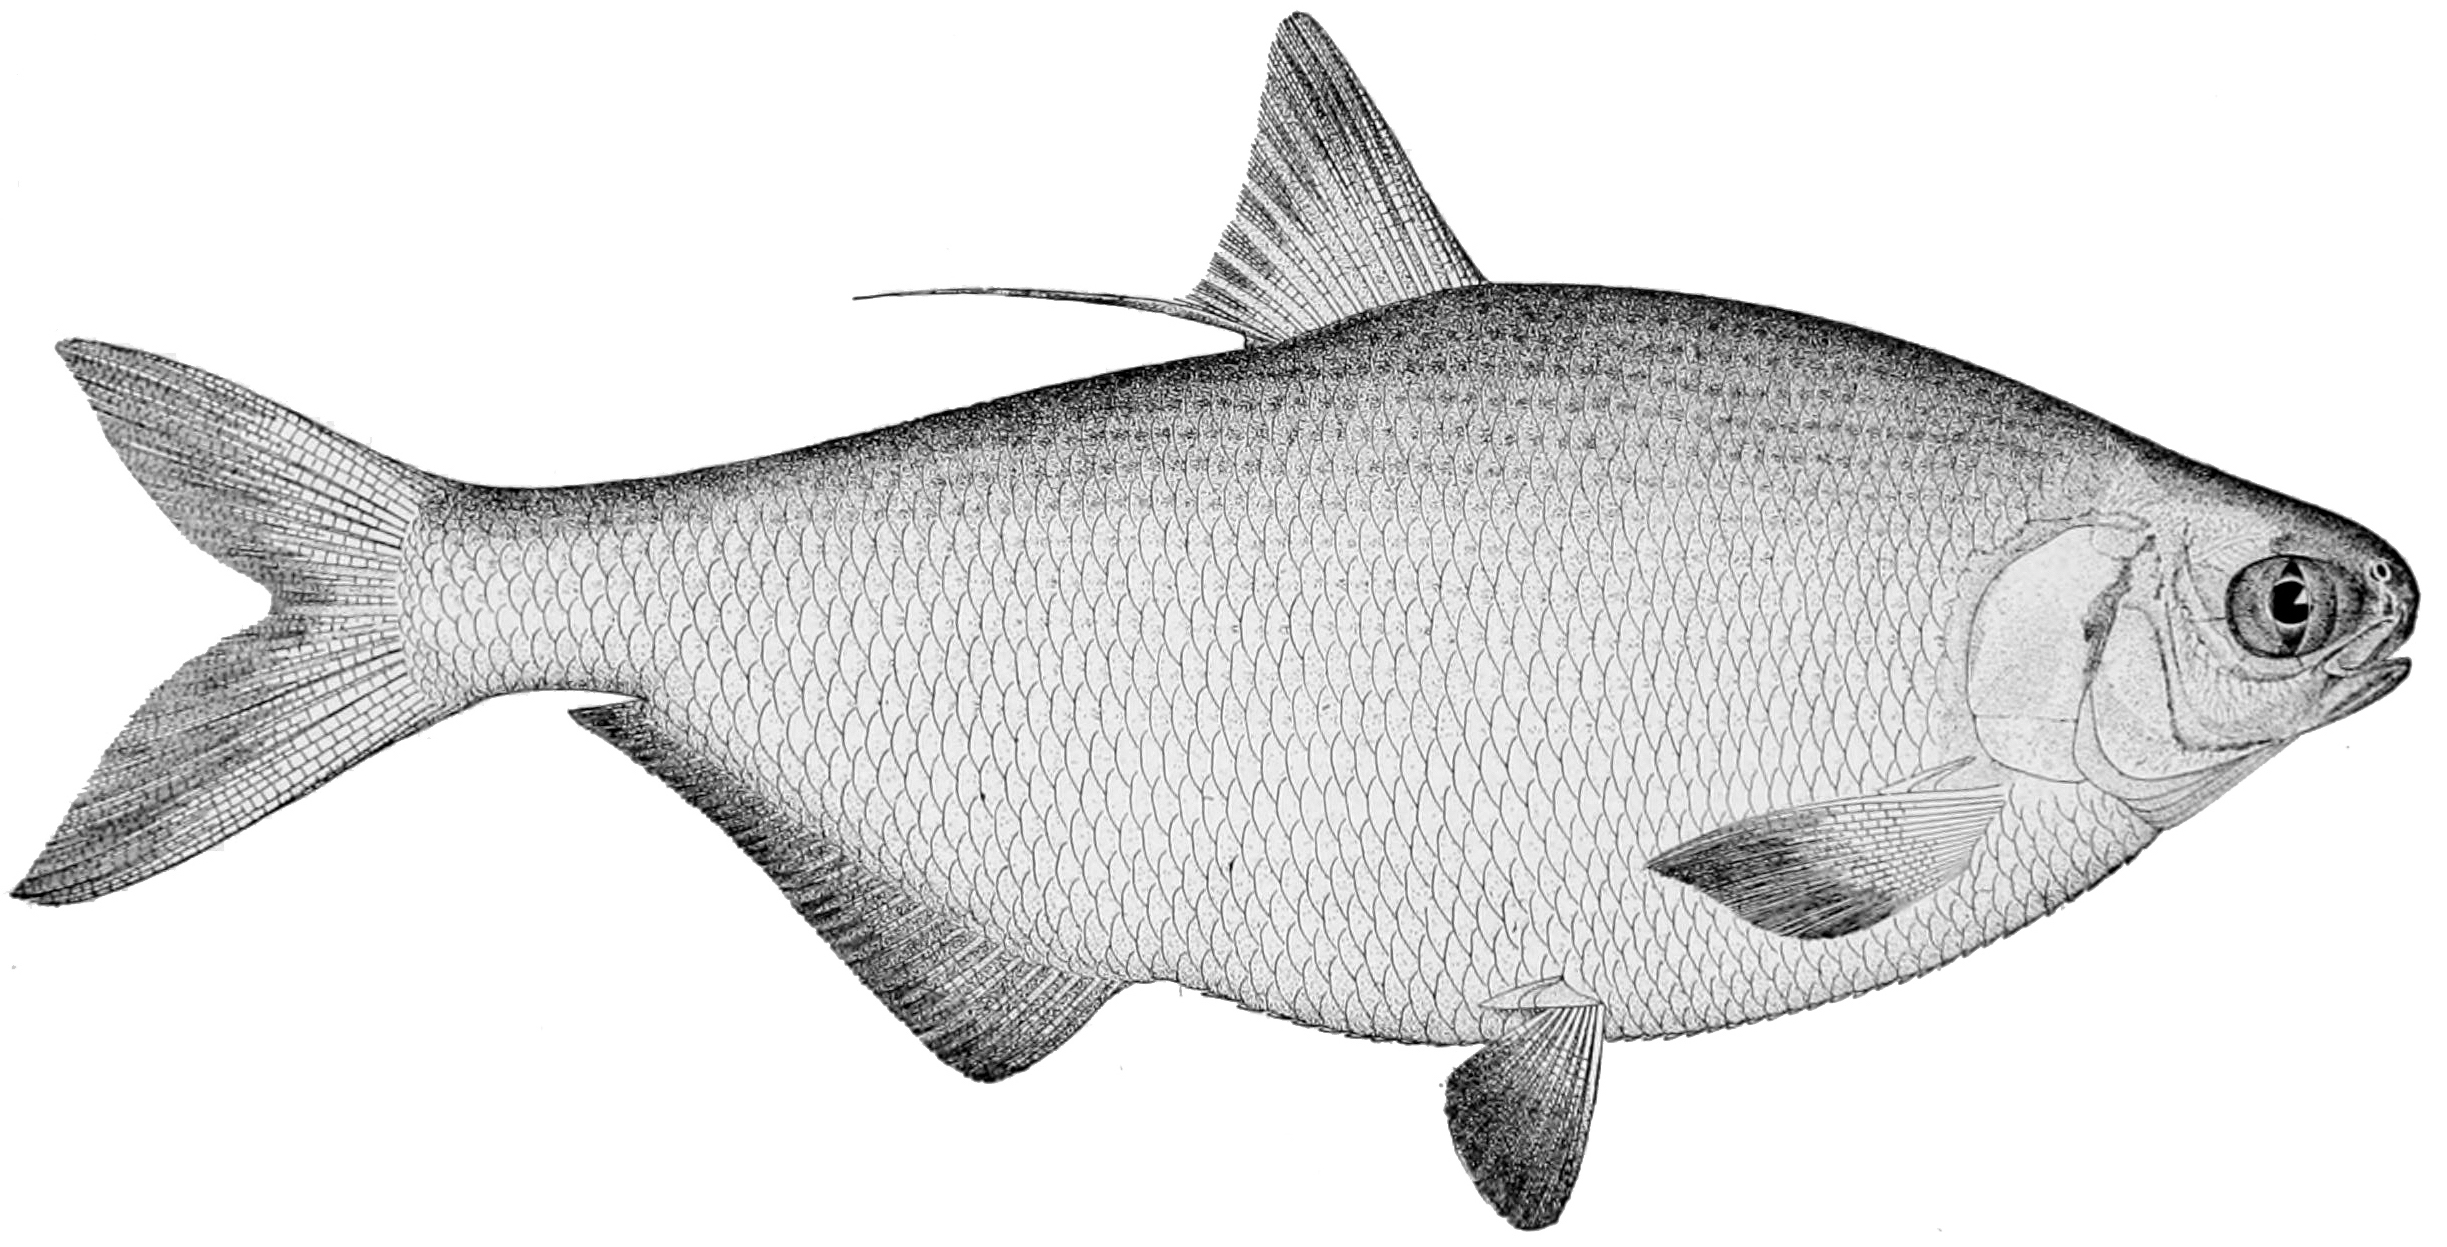
\includegraphics[width=0.12\textwidth]{adult.jpeg} \\
        $n(z,t)$};
\node[align=center] (repro) at (3.25,3) {Reproduction\\
        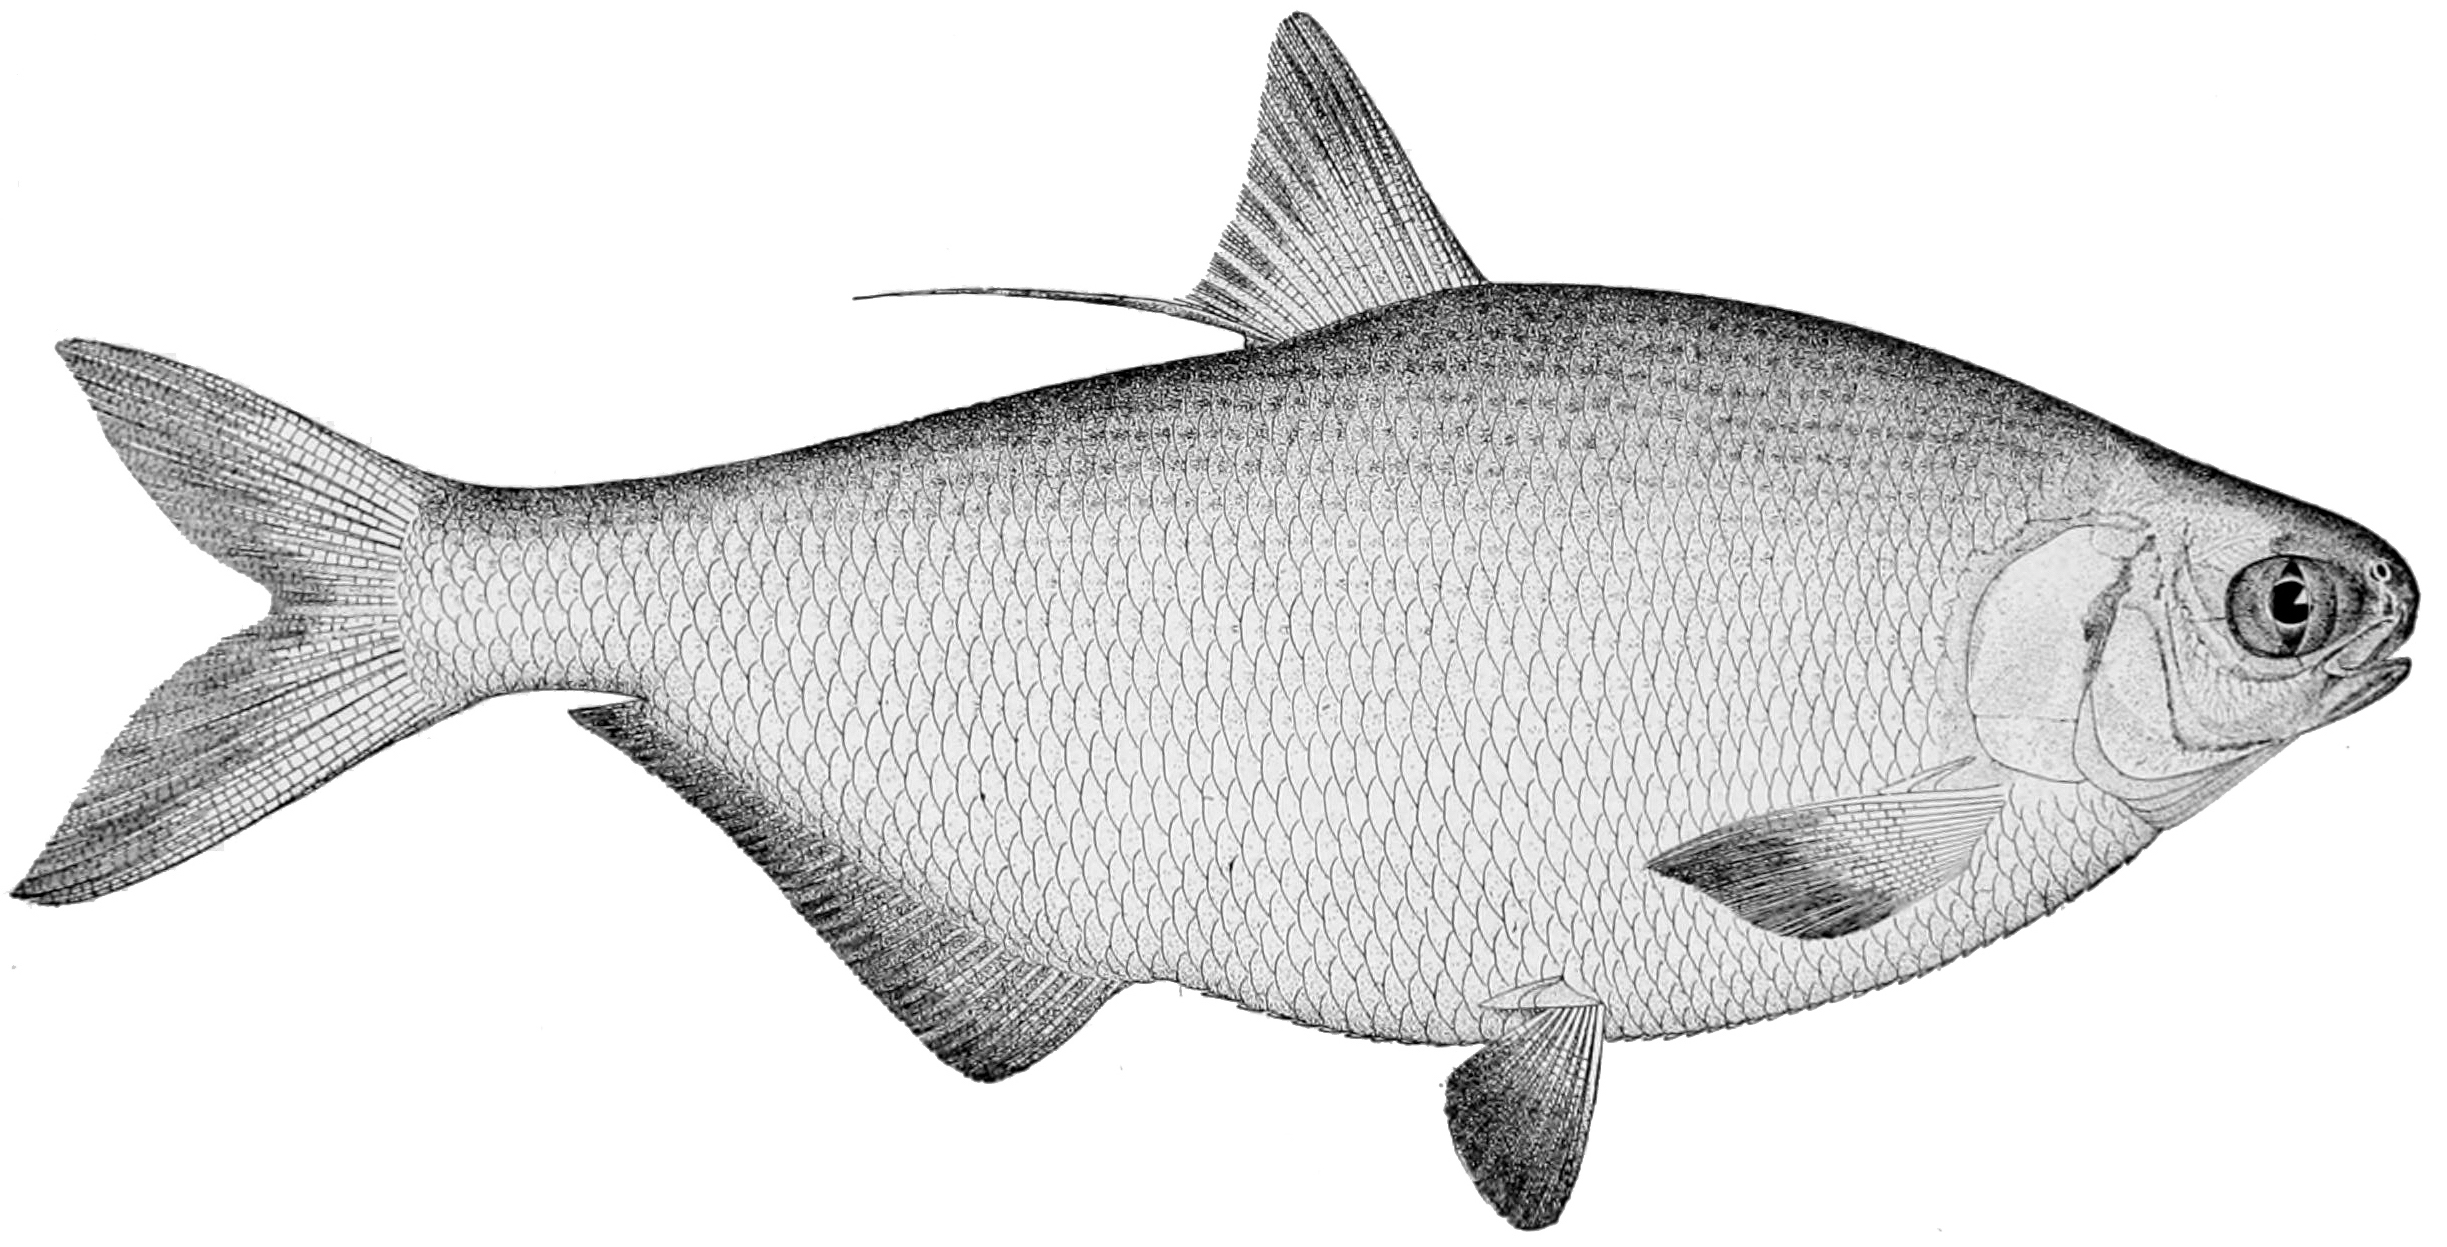
\includegraphics[width=0.12\textwidth]{adult.jpeg}\\
        };
\node (repro_in) at (2.3, 3)  {};
\node (repro_out) at (4.25, 3)  {};
\node (repro_down) at (3, 2.5)  {};
%\node[align=center] (surv) at (4.5,3) {\\
%        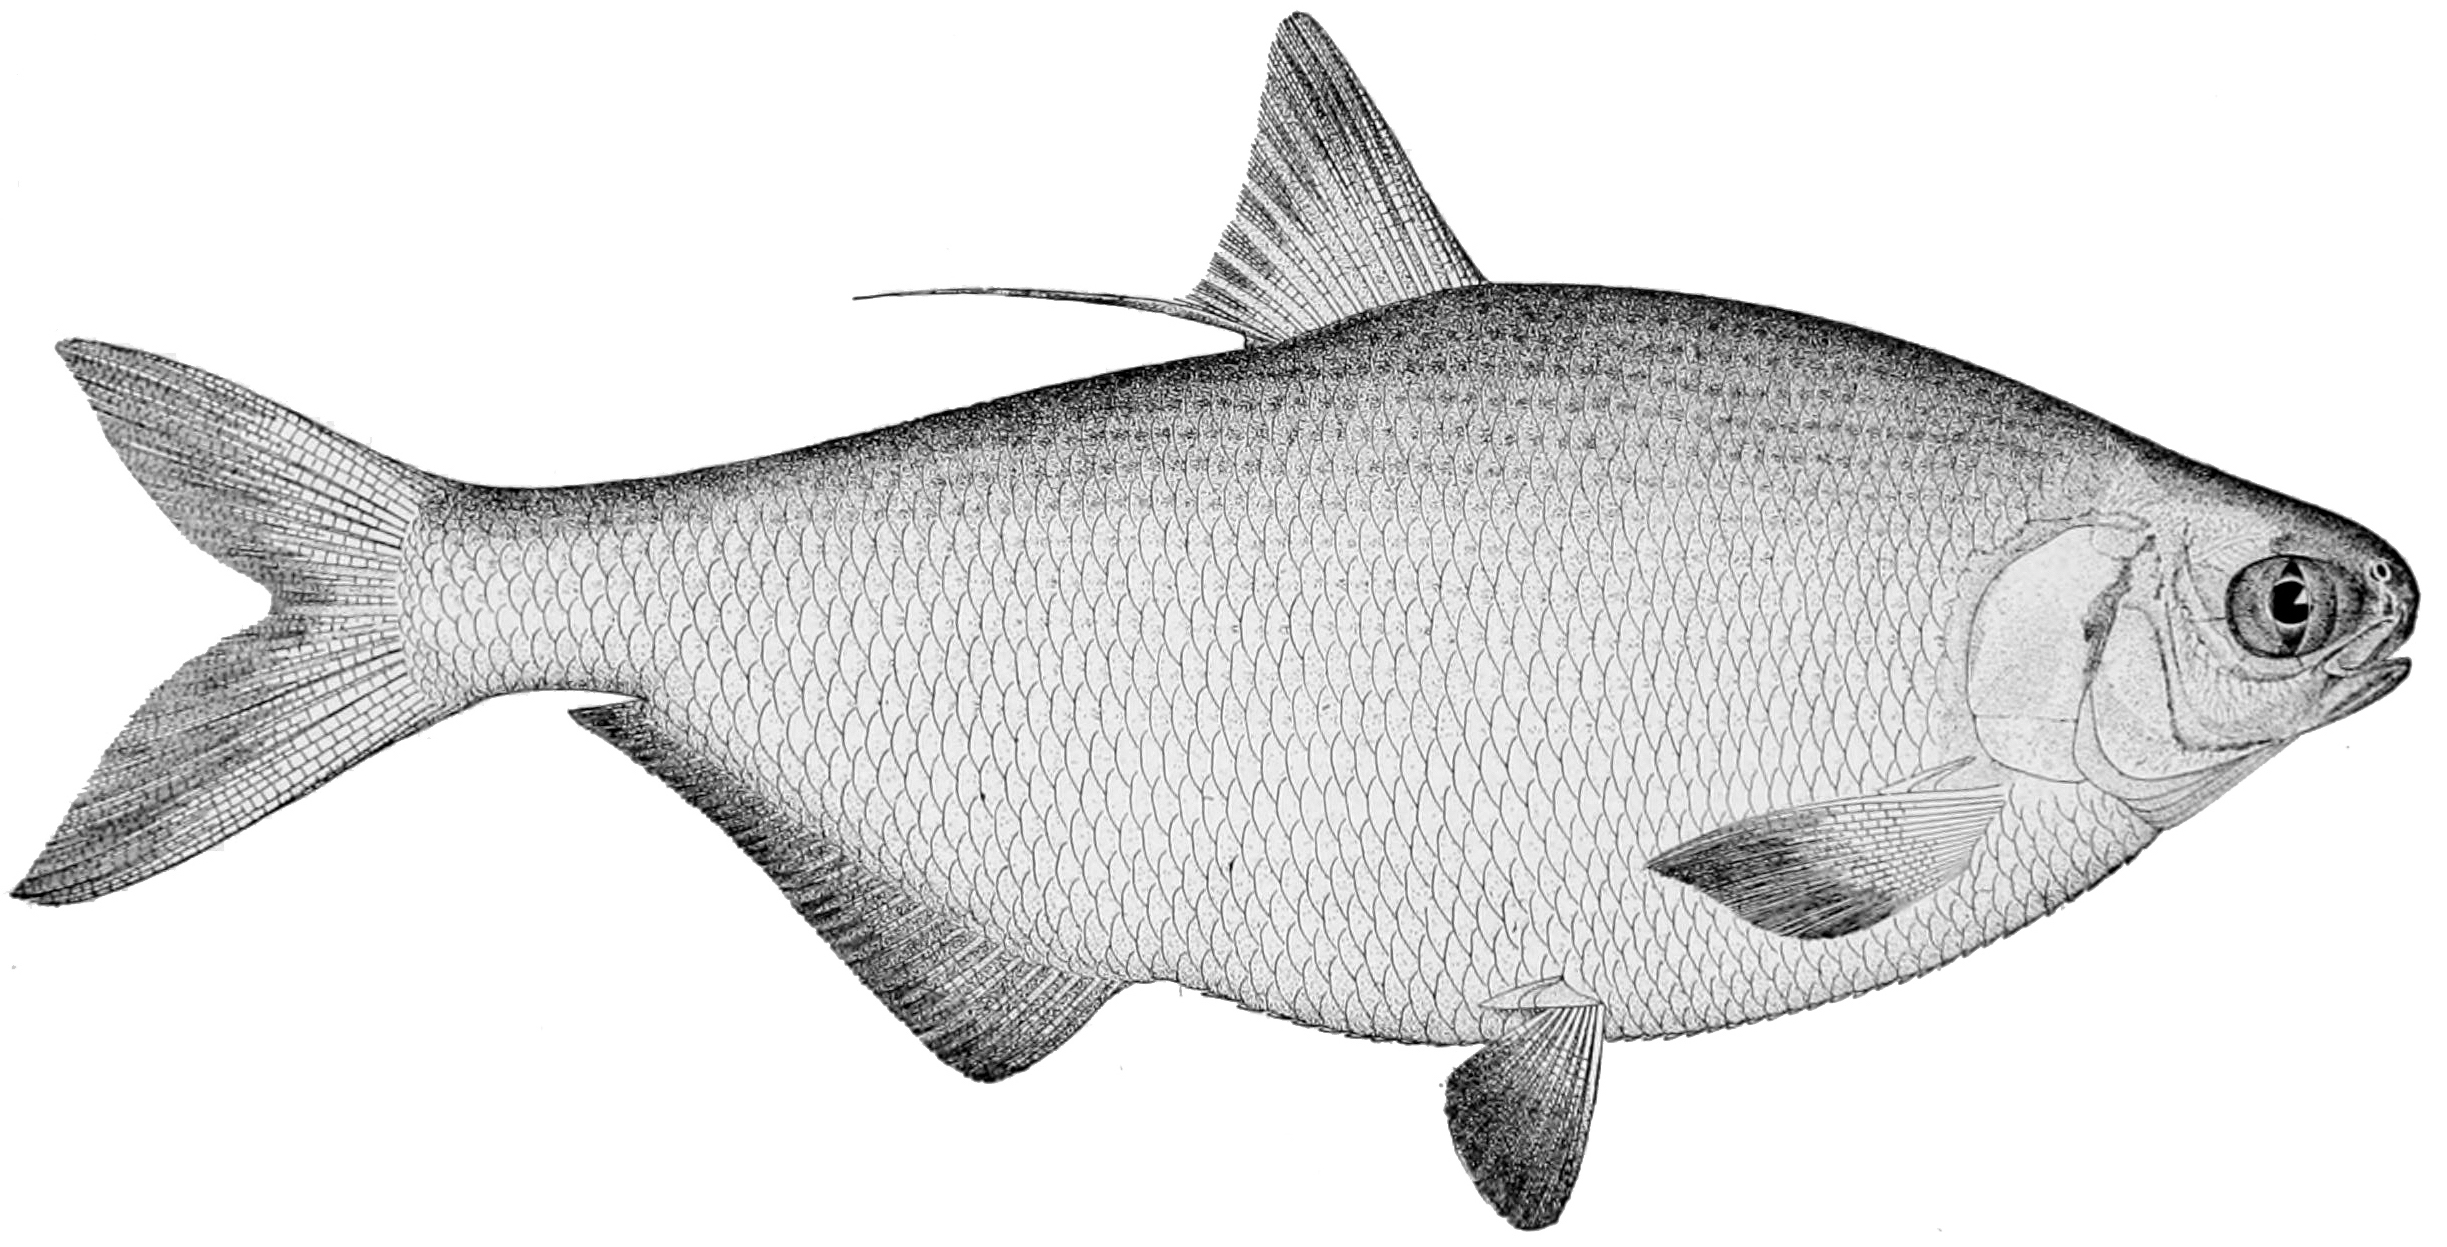
\includegraphics[width=0.15\textwidth]{adult.jpeg}\\
%        };
\node (grow_box) at (6.6,3.85) {Survival \& Growth};
\node[main node, align=center] (census_next) at (10,3) {Census $t+1$ \\
        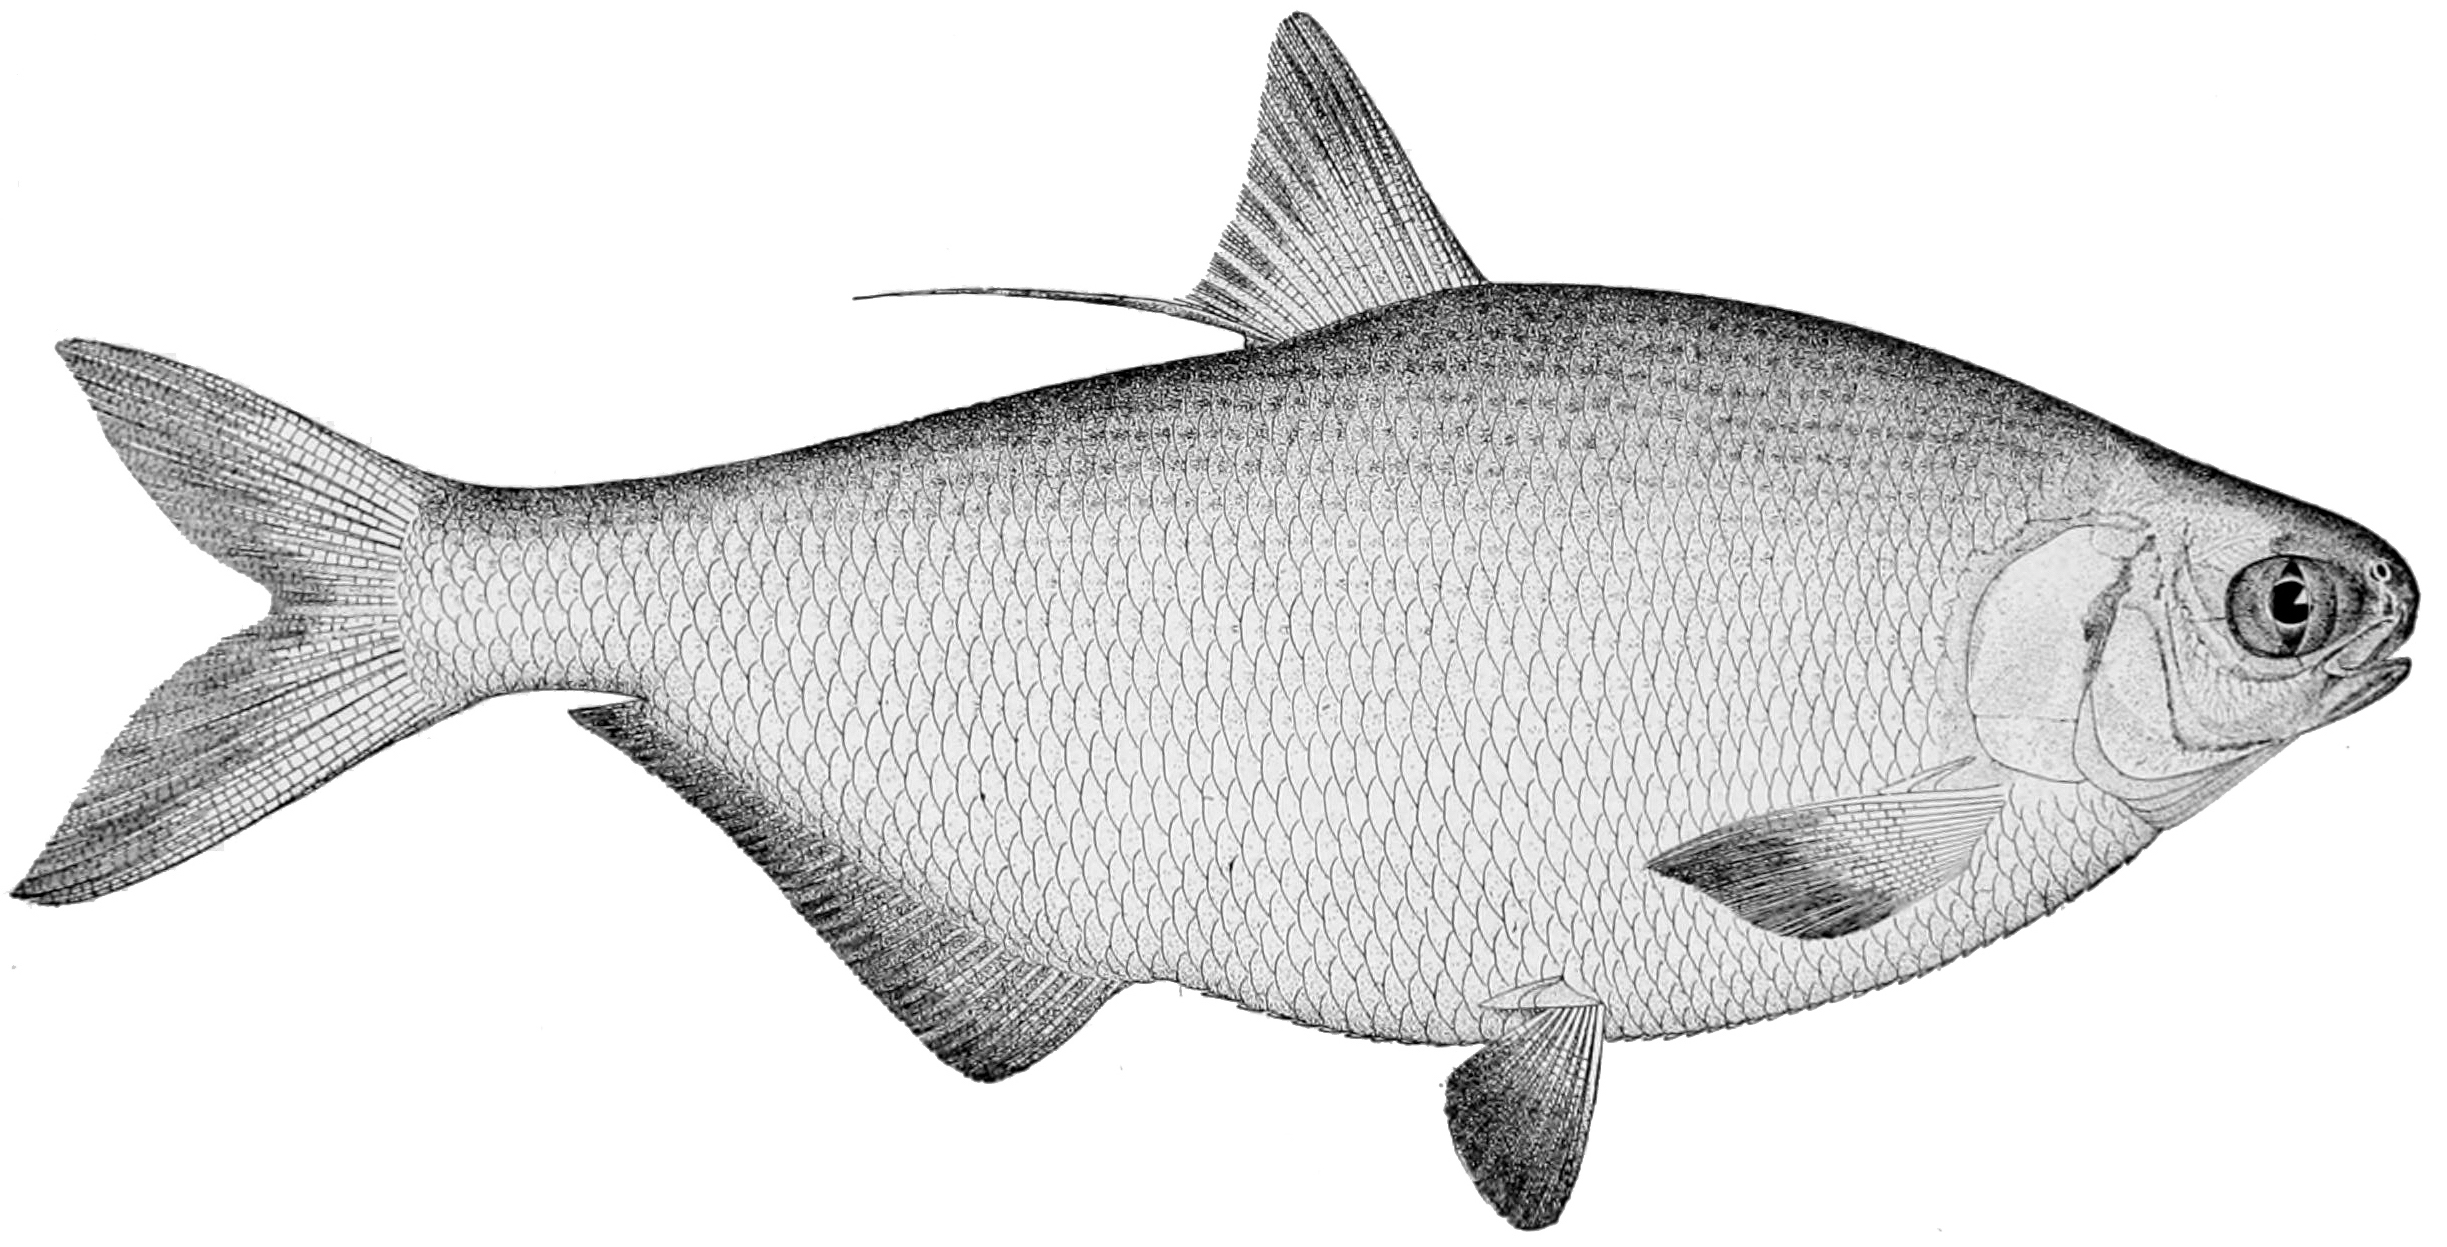
\includegraphics[width=0.15\textwidth]{adult.jpeg}\\
        $n(z',t+1)$};
\node (repro_box) at (13,3.85)  {Reproduction};
\node[align=center] (eggs) at (3,0) {Eggs \\ $\bullet$ $\bullet$ $\bullet$ $\bullet$ \\
  \, $\bullet$ $\bullet$ $\bullet$ $\bullet$ \\ $\bullet$ $\bullet$ $\bullet$ $\bullet$};
  \node[align=center] (eggs_viable) at (5,0) {Viable \\ $\bullet$ $\bullet$ $\bullet$ \\
  \, $\bullet$ $\bullet$ \\ $\bullet$ $\bullet$ $\bullet$};
 \node[align=center] (age1) at (8,0) { Age-1\\
        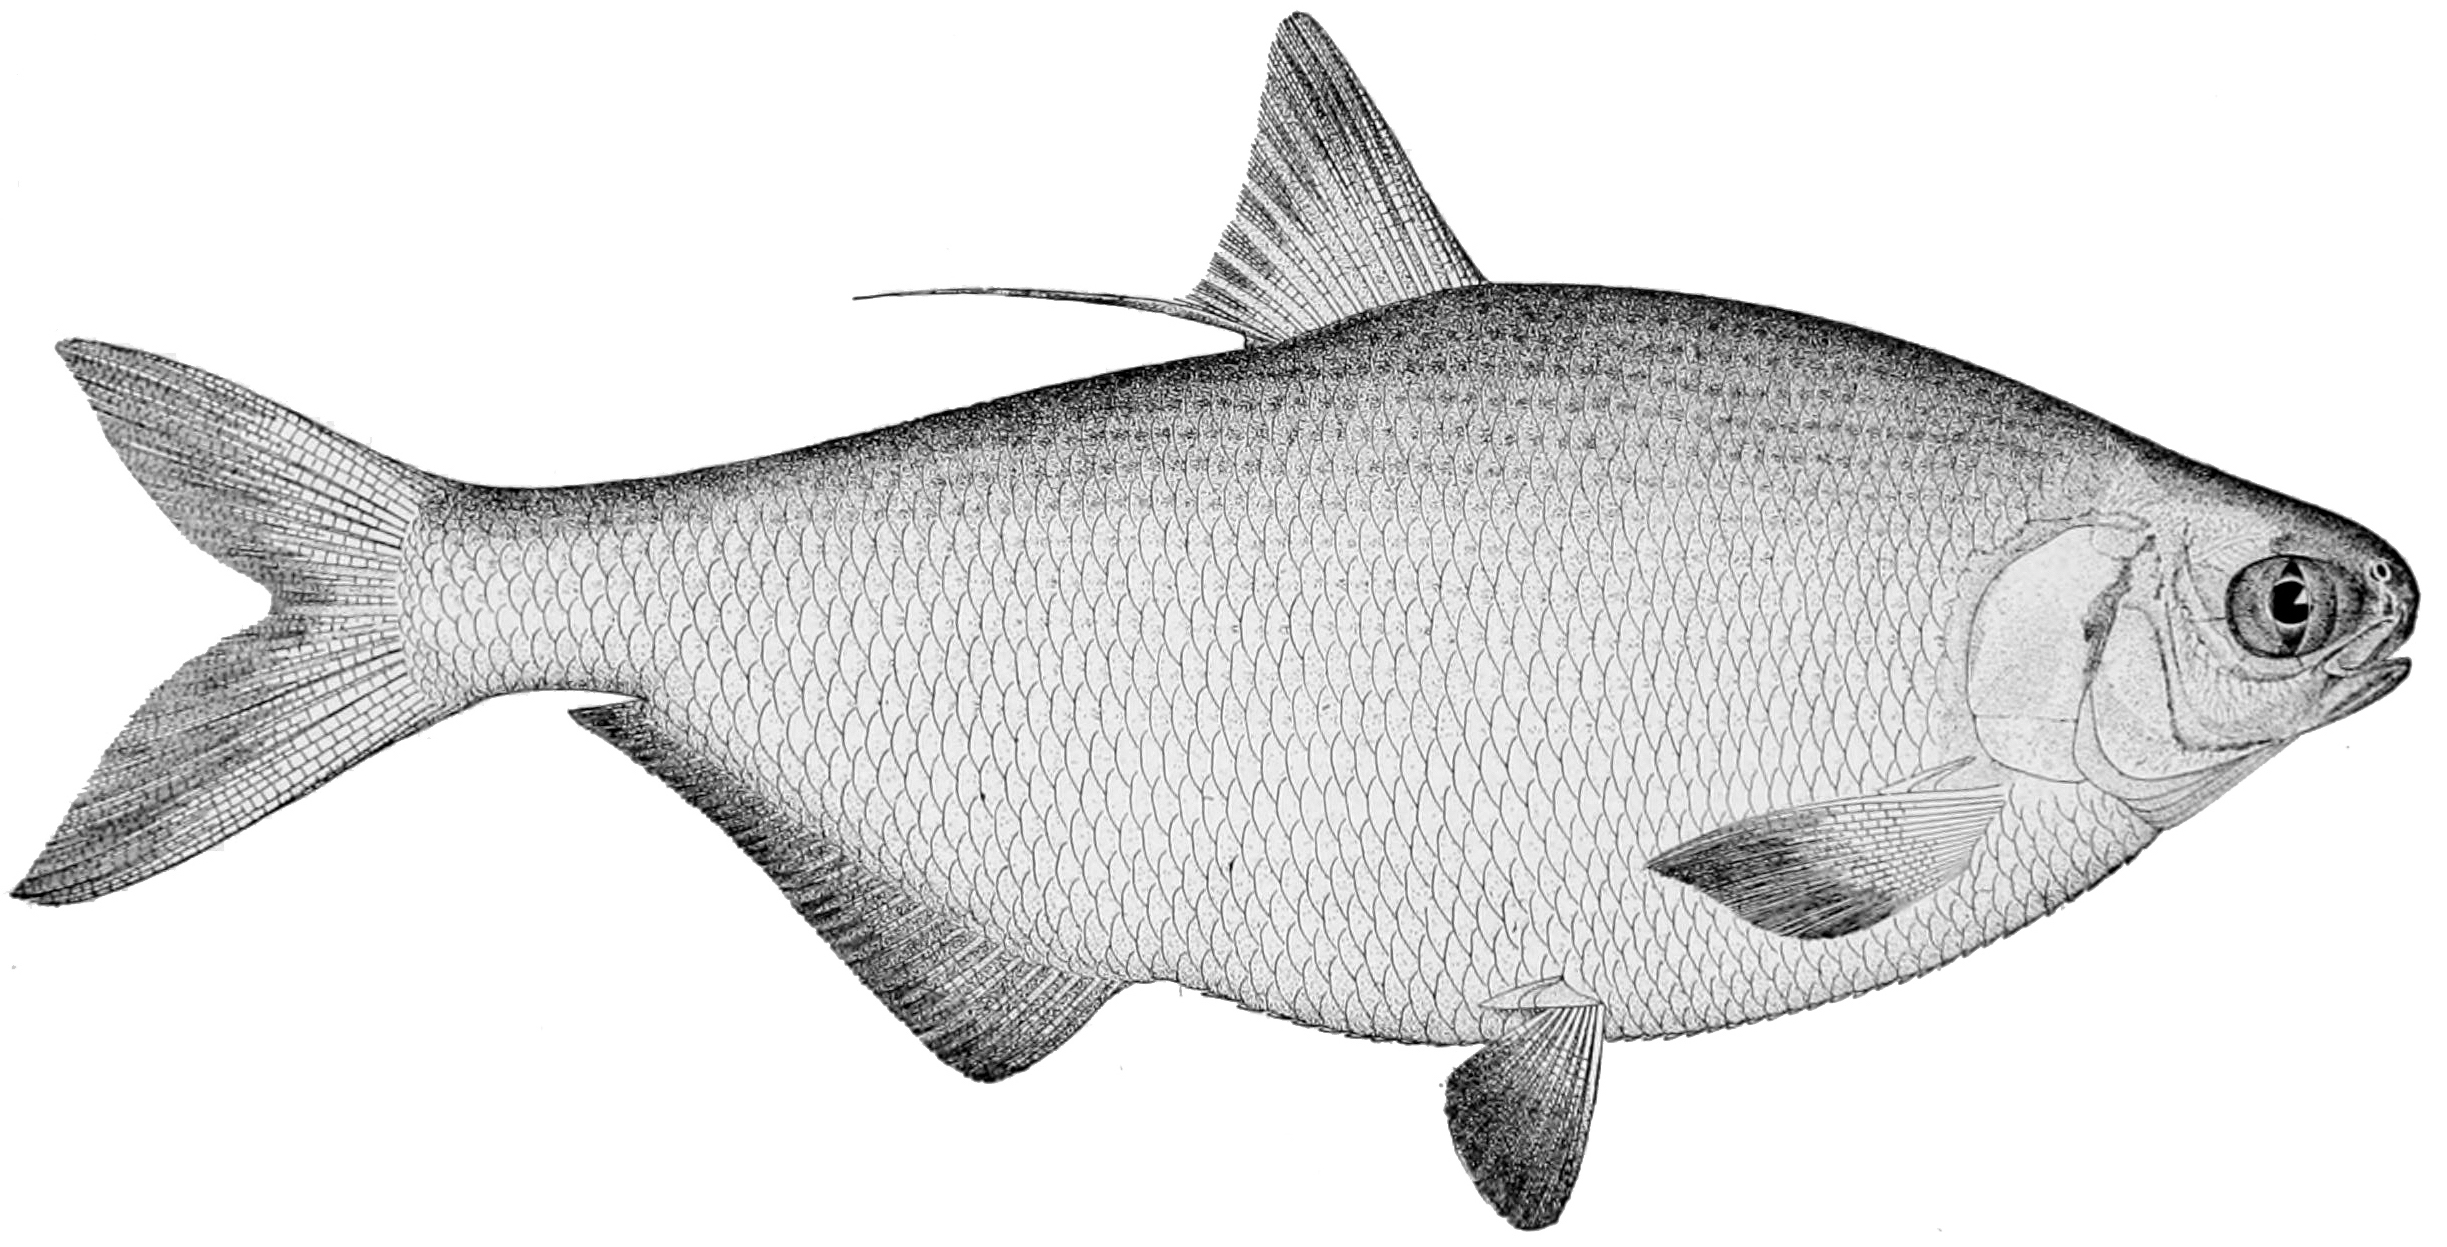
\includegraphics[width=0.06\textwidth]{adult.jpeg}
         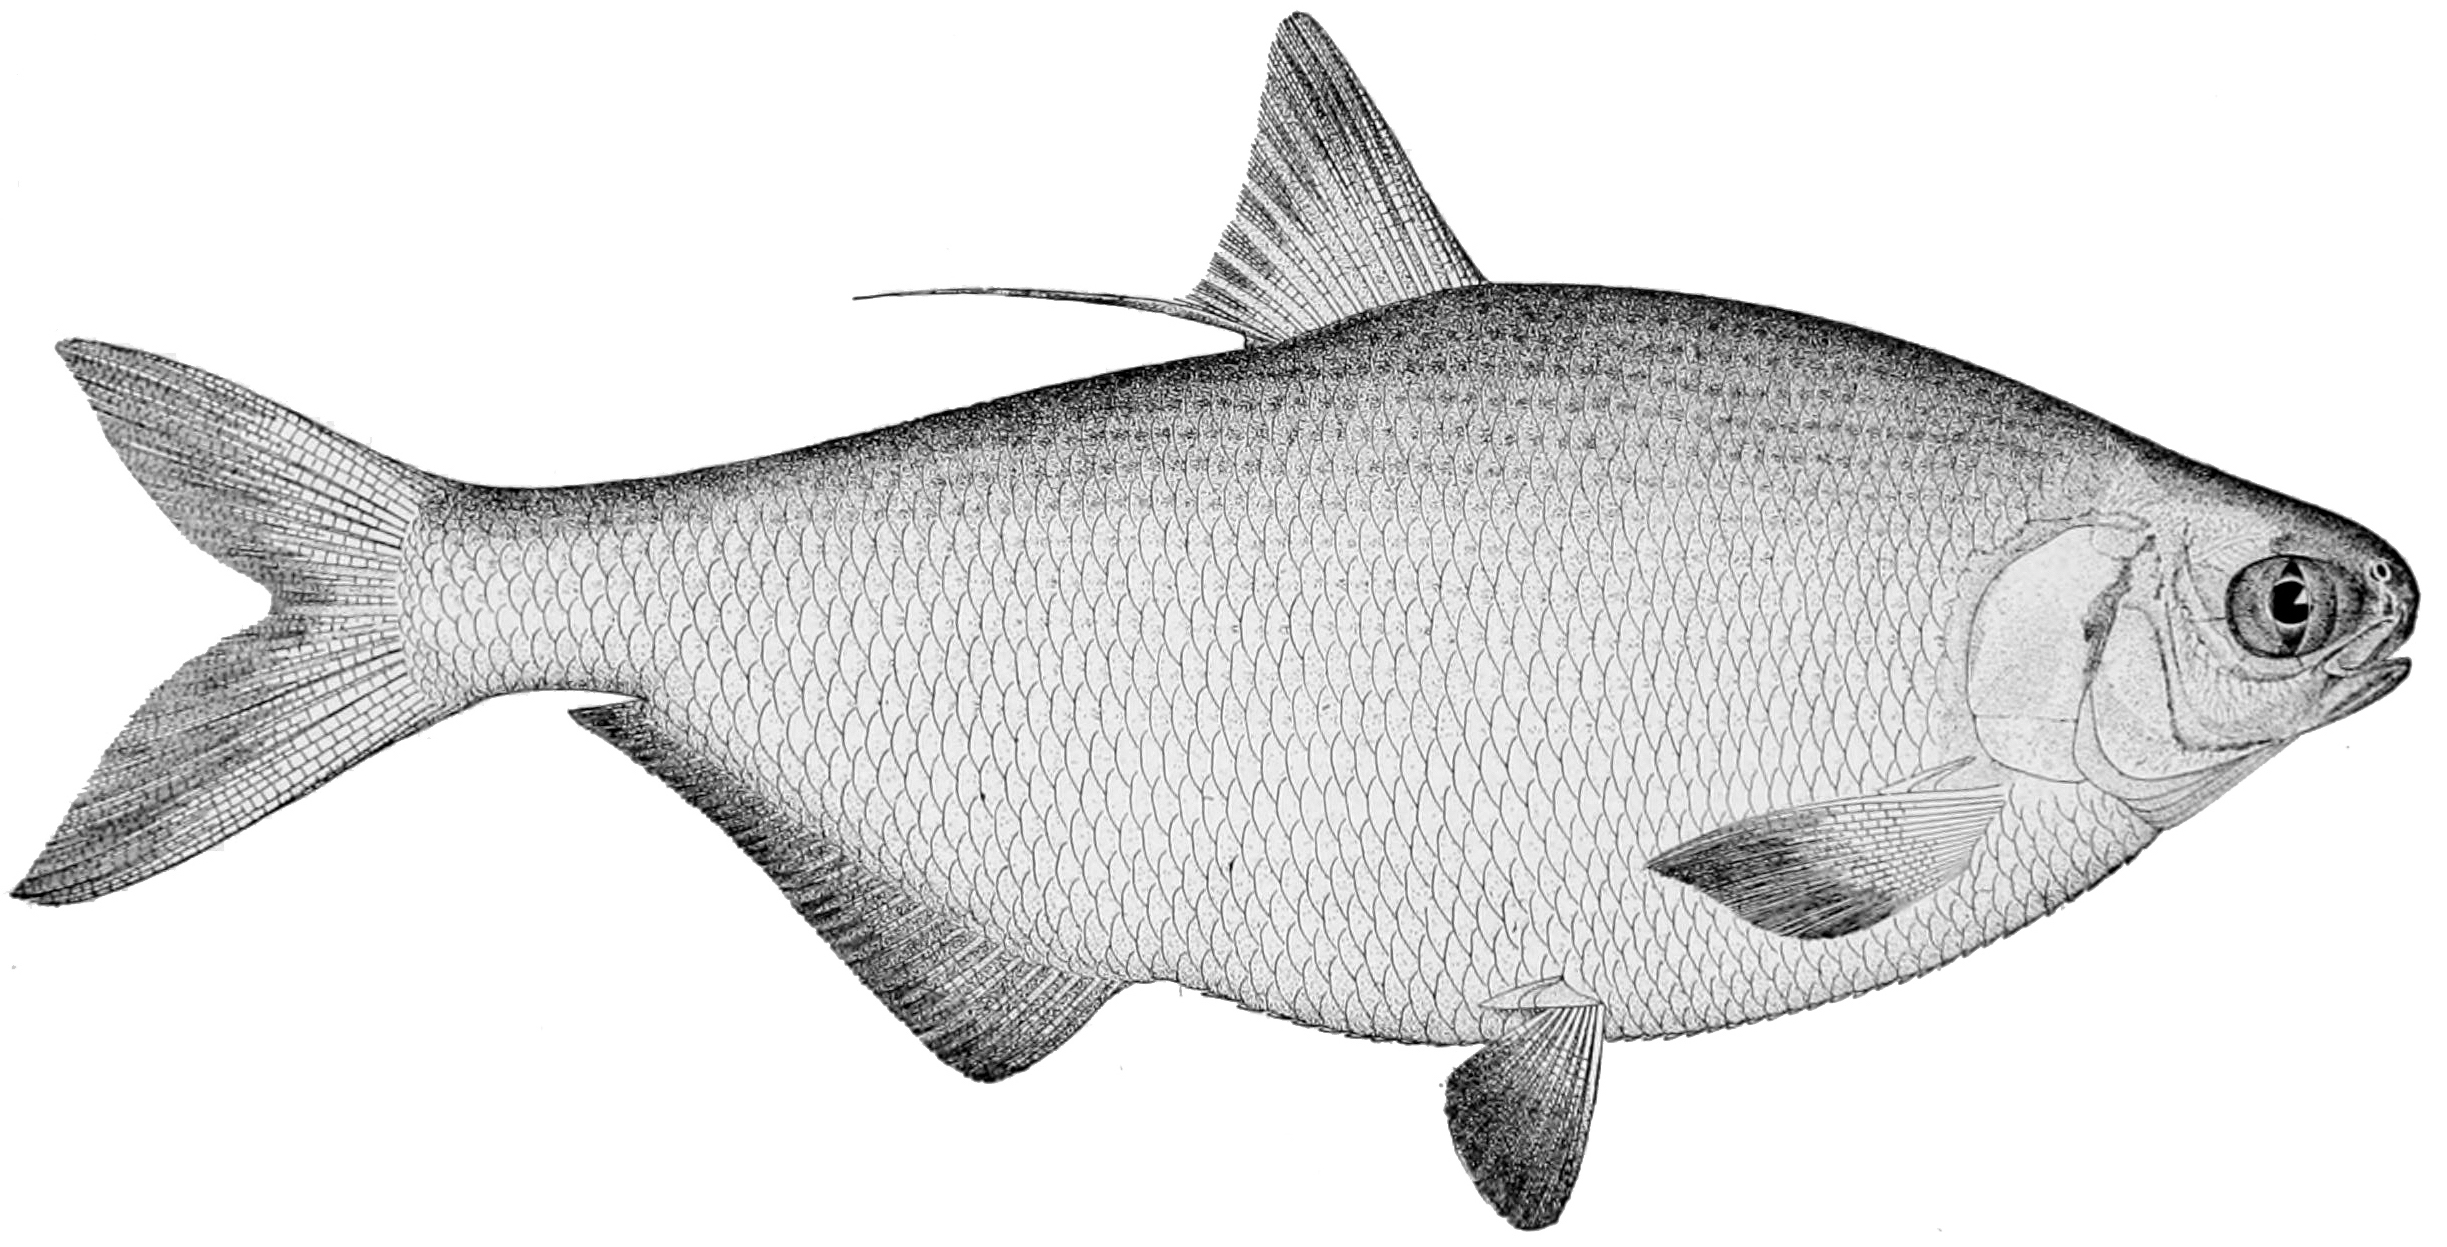
\includegraphics[width=0.04\textwidth]{adult.jpeg}\\
         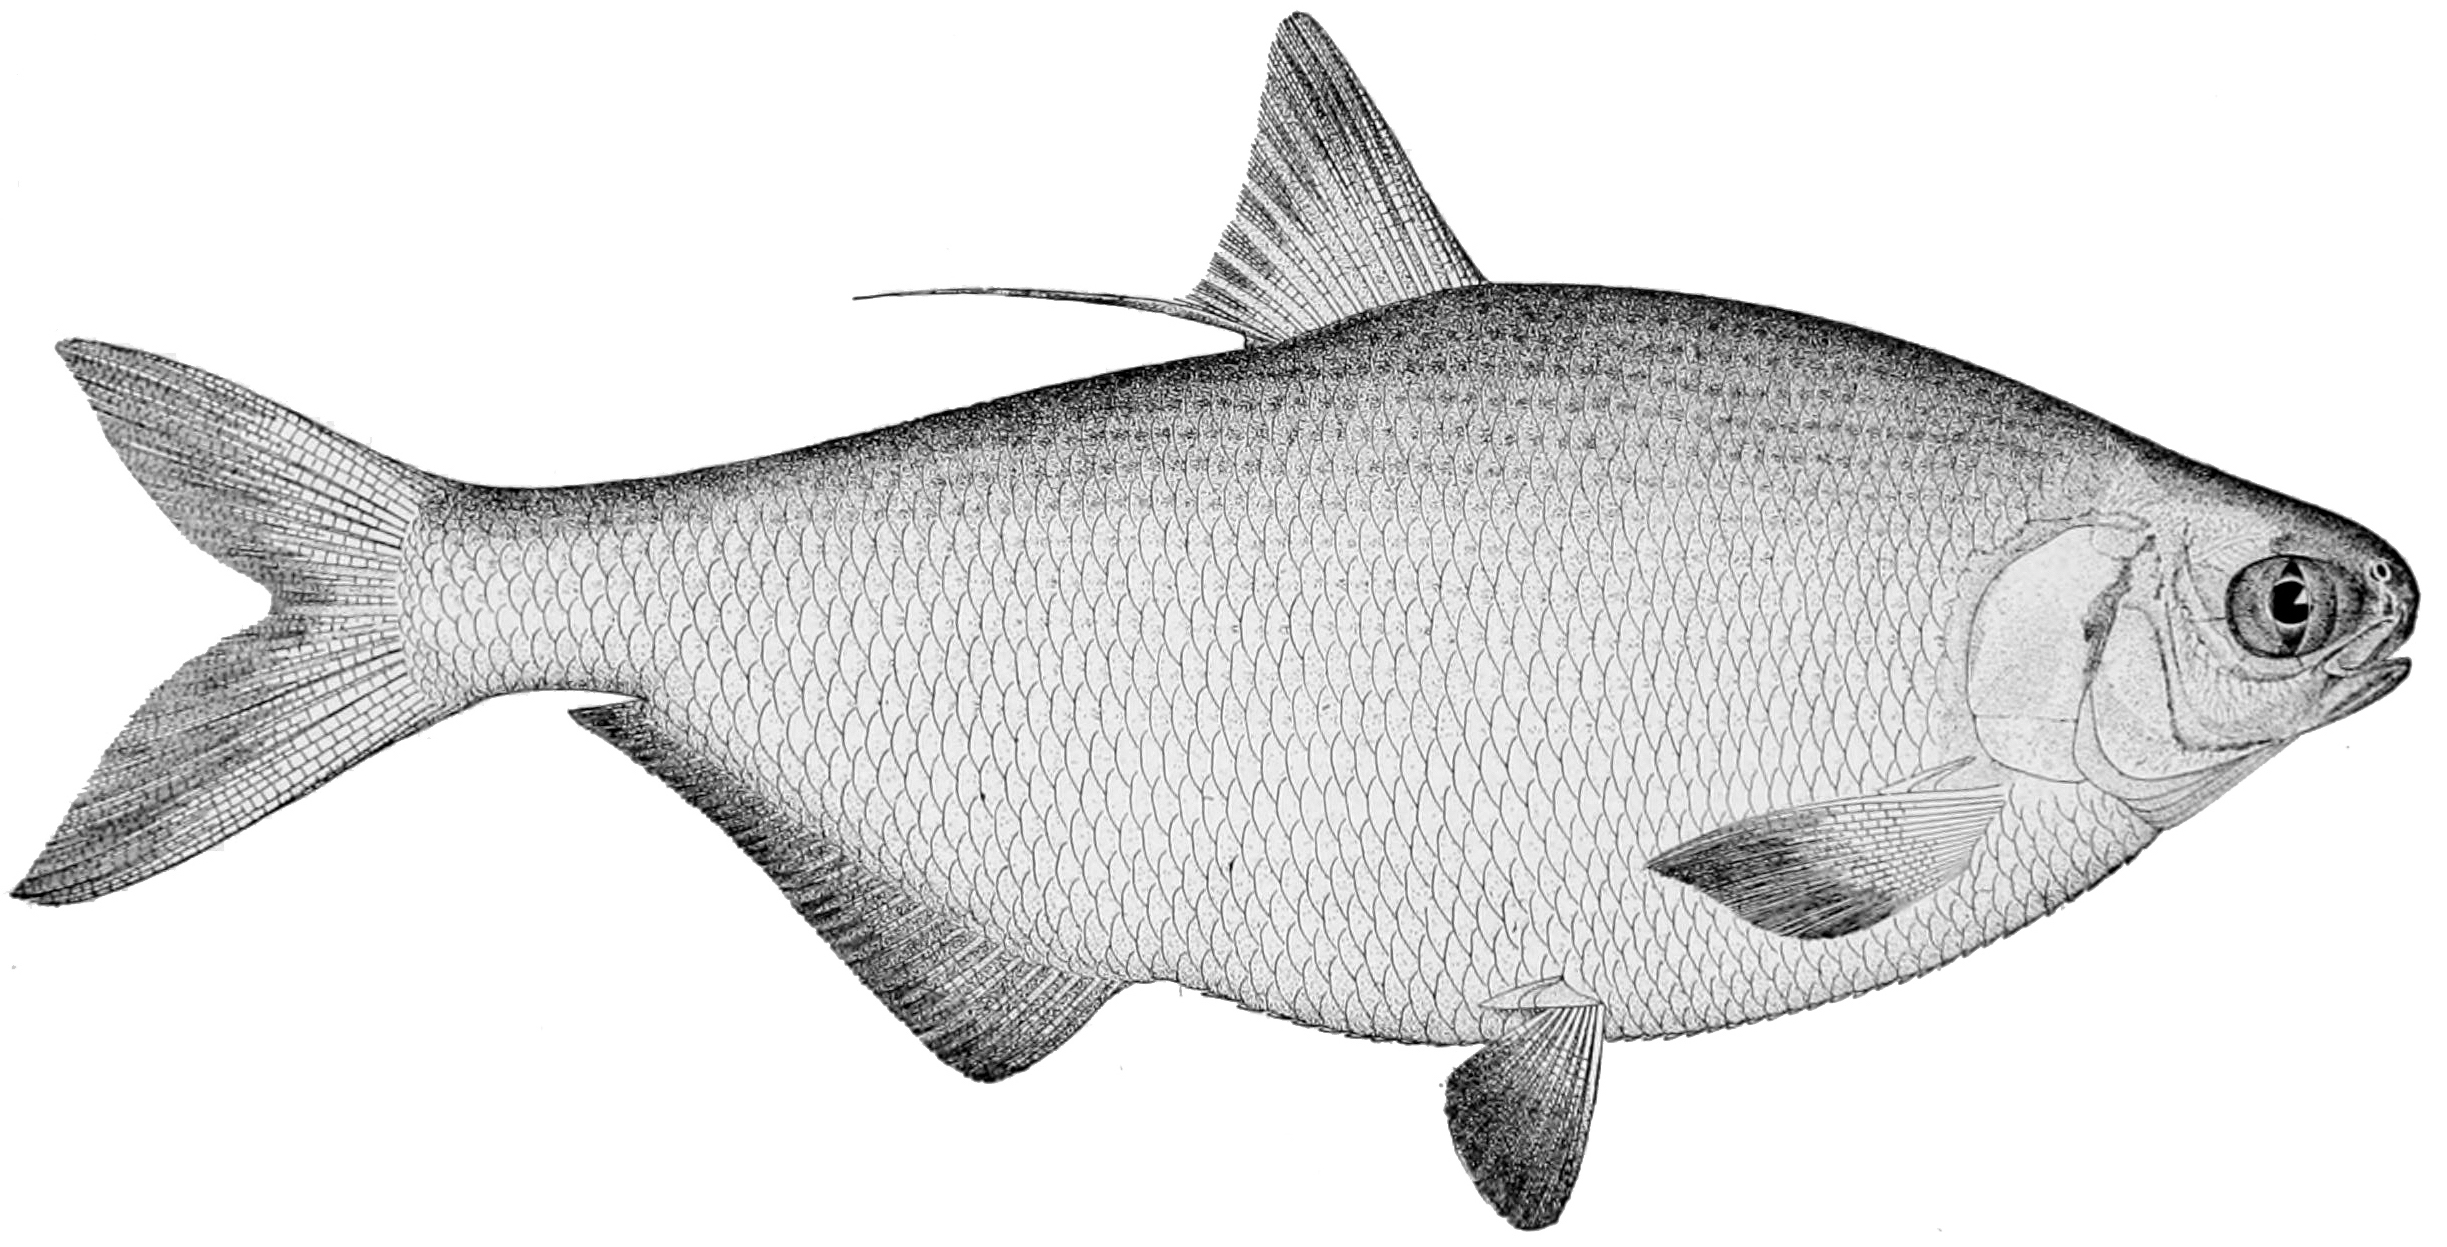
\includegraphics[width=0.08\textwidth]{adult.jpeg}
        };
\node[] (next) at (13,3) {};

\path[->]
	(census_pres) edge node {} (repro_in)
	(repro_out) edge node {$s(z)G(z',z)$} (census_next)
	(census_next) edge node {} (next)
	(repro_down) edge node {$p_b \rm{egg}(z)$} (eggs)
	(eggs) edge node {$\nu$} (eggs_viable)
	(eggs_viable) edge node {$s_0(d)$} (age1)
	(age1) edge node[right, pos=0.3] {$C_1(z')$} (census_next);
	
\end{tikzpicture}
%}
\end{center}
 \caption{\small{Life cycle diagram and census points for pre-reproduction census of gizzard shad.}}
 \label{life_cycle}
\end{figure*}

\subsubsection{Growth and survival}
For an individual of length $z$ at time $t$, $P(z',z)\Delta z$ is the probability that the individual is alive at time $t+1$, and its size is in the interval $[z', z' + \Delta z]$ (as with $n(z,t)$ this is an approximation that is valid for small $\Delta z$, and the exact probability is given by an integral like the one above). We define $P(z', z) = s(z)G(z',z)$ where $s(z)$ is the annual adult survival probability and the growth $G(z',z)$ describes the annual length transitions. 
The survival function is a logistic function,
\begin{equation}\label{eq:surv}
s(z) = s_{\rm min} + \frac{s_{\rm max}-s_{\rm min}}{1+e^{\beta_s(\ln(z)-\ln(\alpha_s))}},
\end{equation}
with four parameters: the minimum survival rate $s_{\rm min}$; a maximum survival rate, $s_{\rm max}$; an intercept parameter, $\alpha_{s}$; and a slope parameter, $\beta_{s}$ \citep{bolker2008ecological}.  
The growth function is a two-variable normal distribution centered around a modified von Bertalanffy function of the length at time t \citep{erickson2017integral}.  
Consequently if $L_\infty$ is maximum asymptotic length and $K_g$ is the individual growth rate of gizzard shad, then the growth kernel
$$\ds G(z',z) = \mathrm{Prob}(z' \, | \,  z, L_{\infty}, K_g) = \mathrm{Normal PDF}(\mu_g, \sigma_g)$$
where $\mu_g =  L_{\infty} \left(1-e^{-K_g} \right) + z(t)e^{-K_g}$ and $\sigma_g$ is the standard deviation.

\subsection{Fecundity}

$F(z',z)\Delta z$ is the number of new offspring in the length interval $[z', z' + \Delta z]$ present at time $t+1$, per length-$z$ individual at time $t$.
The fecundity kernel is
\begin{equation}\label{eq:fecundity}
F(z', z) = p_b \, \mbox{egg}(z) \, \nu \, s_0(d(t)) \, C_1(z')
\end{equation}
where $p_b$ is the probability of reproducing, $\mbox{egg}(z)$ is the mean number of eggs produced, $\nu$ is the probability that an egg is viable, $s_0(d(t))$ is the density-dependent probability of surviving to age-1, and $C_1 (z')$ is the length distribution of new recruits at age-1 (when they are first censused in the model).

The mean number of eggs produced by females of a certain length is a three-parameter logistic function,
\begin{equation}\label{eq:egg}
\mbox{egg}(z) = \frac{\mbox{egg}_{\rm max}}{1+e^{\beta_e(\ln(z)-\ln(\alpha_e))}}.
\end{equation}

The probability of gizzard shad survival during their first year can depend on many factors \citep{michaletz2010overwinter} including predation, temperature, the mean total length of fish, and the density of age-0 fish.  
In this study, we focused only on the density factor and assumed the probability of survival of age-0 fish is the exponential function,
\begin{equation}\label{eq:s0}
s_0(d(t)) = a_0 \, e^{-b_0 d(t)},
\end{equation}
where $a_0$ is the intercept, $b_0$ the decay rate, and $d(t)$ is the density at time $t$ of age-0 gizzard shad per 1000 m$^3$, 
\[ d(t) = 10^{-3} \int_L^U p_b \, \mbox{egg}(z) \, \nu n(z,t) \, dz. \]  

Finally, the total number of eggs that survive to be an age-1 fish is multiplied with a normal distribution of length,
$ \ds C_1 (z') =  \mathrm{Normal PDF} (\mu_r, \sigma_r)$ where $\mu_r$ is the mean length of age-1 gizzard shad and $\sigma_r$ is the standard deviation. 

\subsection{Dynamical model} 
The population at time $t+1$ is the sum of the contributions from each individual alive at time $t$,
\begin{equation}\label{eq:IPM}
n(z',t+1) = \int_L^U K(z',z)n(z,t) \,dz,
\end{equation}  
where $K(z',z) = s(z) G(z',z) + F(z',z)$ and $[L,U]$ is the range of all possible lengths.

\section{Methods}
\subsection{LTRM data and model parameterization} \label{LTRM}
The LTRM element of the Upper Mississippi River Restoration monitors the UMRS to provide an understanding of the system's ecology, resource changes, and inform management \citep{bouska2018developing, UMRR2015}.
In order to achieve this goal, numerous features of the UMRS, such as aquatic vegetation, bathymetry, fish, land use/land cover, and water quality are continually surveyed from Navigation Pool 1 (at Minneapolis, Minnesota) south to the confluence of the Mississippi and Ohio Rivers at Cairo, Illinois. 
LTRM fish surveys are conducted at five locations along the main channel of the Upper Mississippi River (Pools 4, 8, 13, 26, and the Open River Reach) and at one location along the Illinois River (La Grange Reach) (Figure \ref{fig:field_stations}). 
Fish are captured using a multiple gear approach (which includes netting and electrofishing) in order to monitor the responses and health of fish communities along these two very important waterways over time \citep{gutreuter1995long}. 
Specific capture methodologies, protocols and modifications to the LTRM can be found in \cite{gutreuter1995long}, and \cite{ickes2002evaluation}. 
In terms of gizzard shad, fish traits (such as total length) have been recorded since 1989 with approximately 3000 collections occurring per year along the Mississippi River (Figure \ref{fig:LTRMmain}). 
For the La Grange Reach of the Illinois River, gizzard shad have been sampled and measured since 1990 with approximately 500 collections occurring per year.

To parameterize our model, we used gizzard shad data collected from the 5 sites along the Mississippi River.  
We then validated our model using empirical information collected from the La Grange Reach of the Illinois River. 
We undertook this approach as the La Grange Reach is upstream of the Mississippi River making it a more distinct location compared to the other sites. 

\begin{figure}
\centering
\begin{subfigure}[b]{.43\textwidth}  
  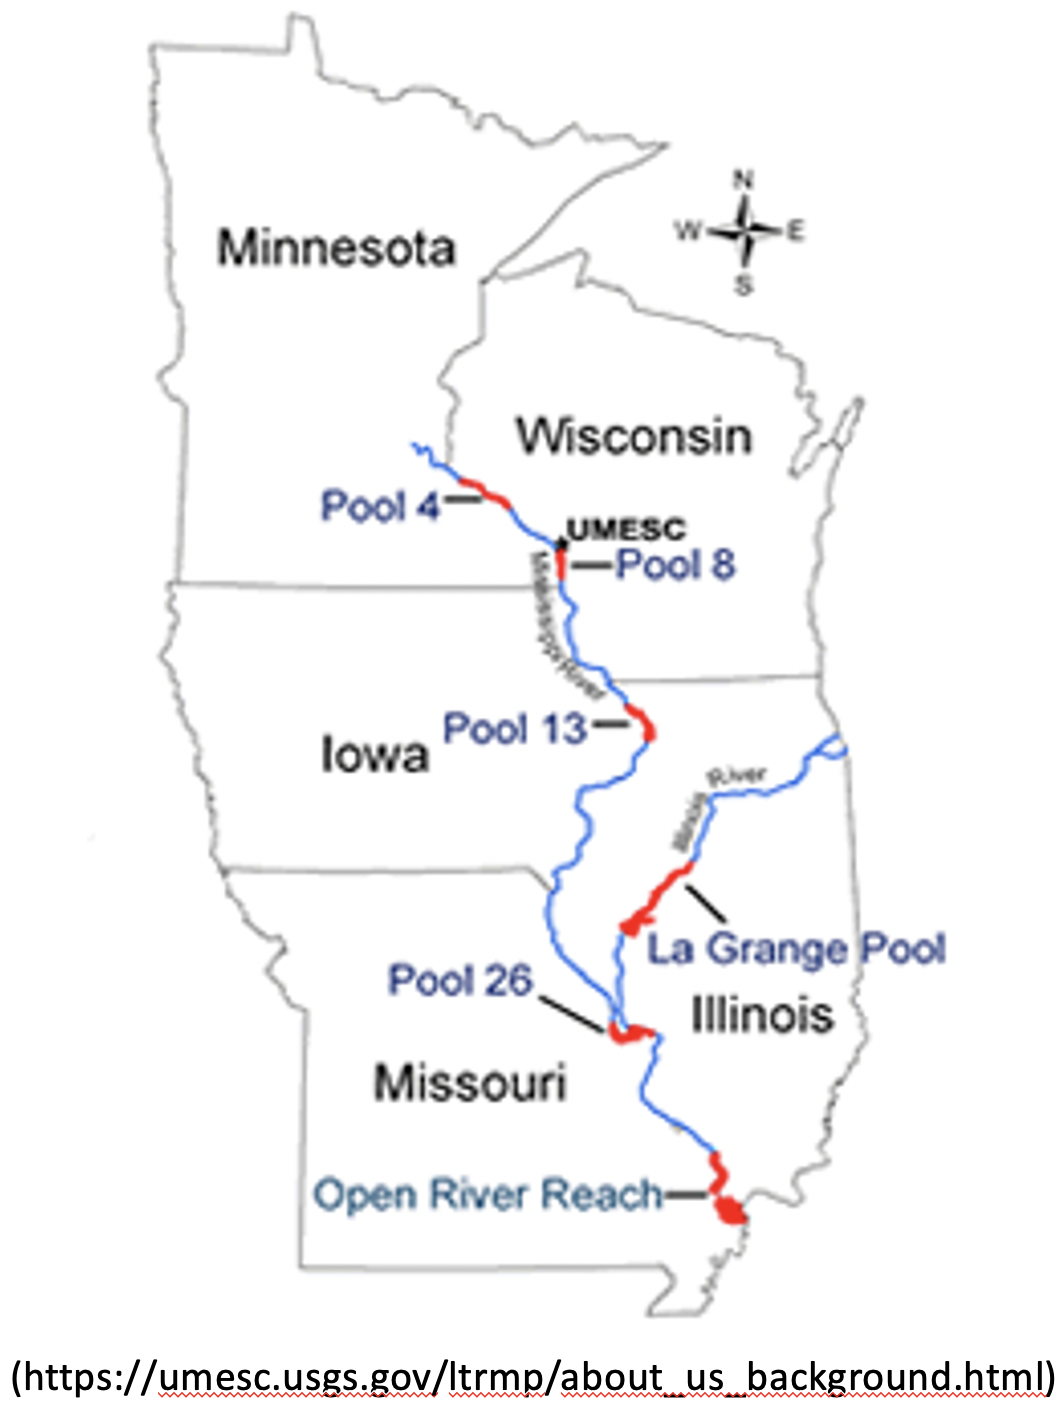
\includegraphics[width=.6\textwidth]{figures/field_stations.png}
  \caption{}
  \label{fig:field_stations}
\end{subfigure}
\begin{subfigure}[b]{.43\textwidth} 
   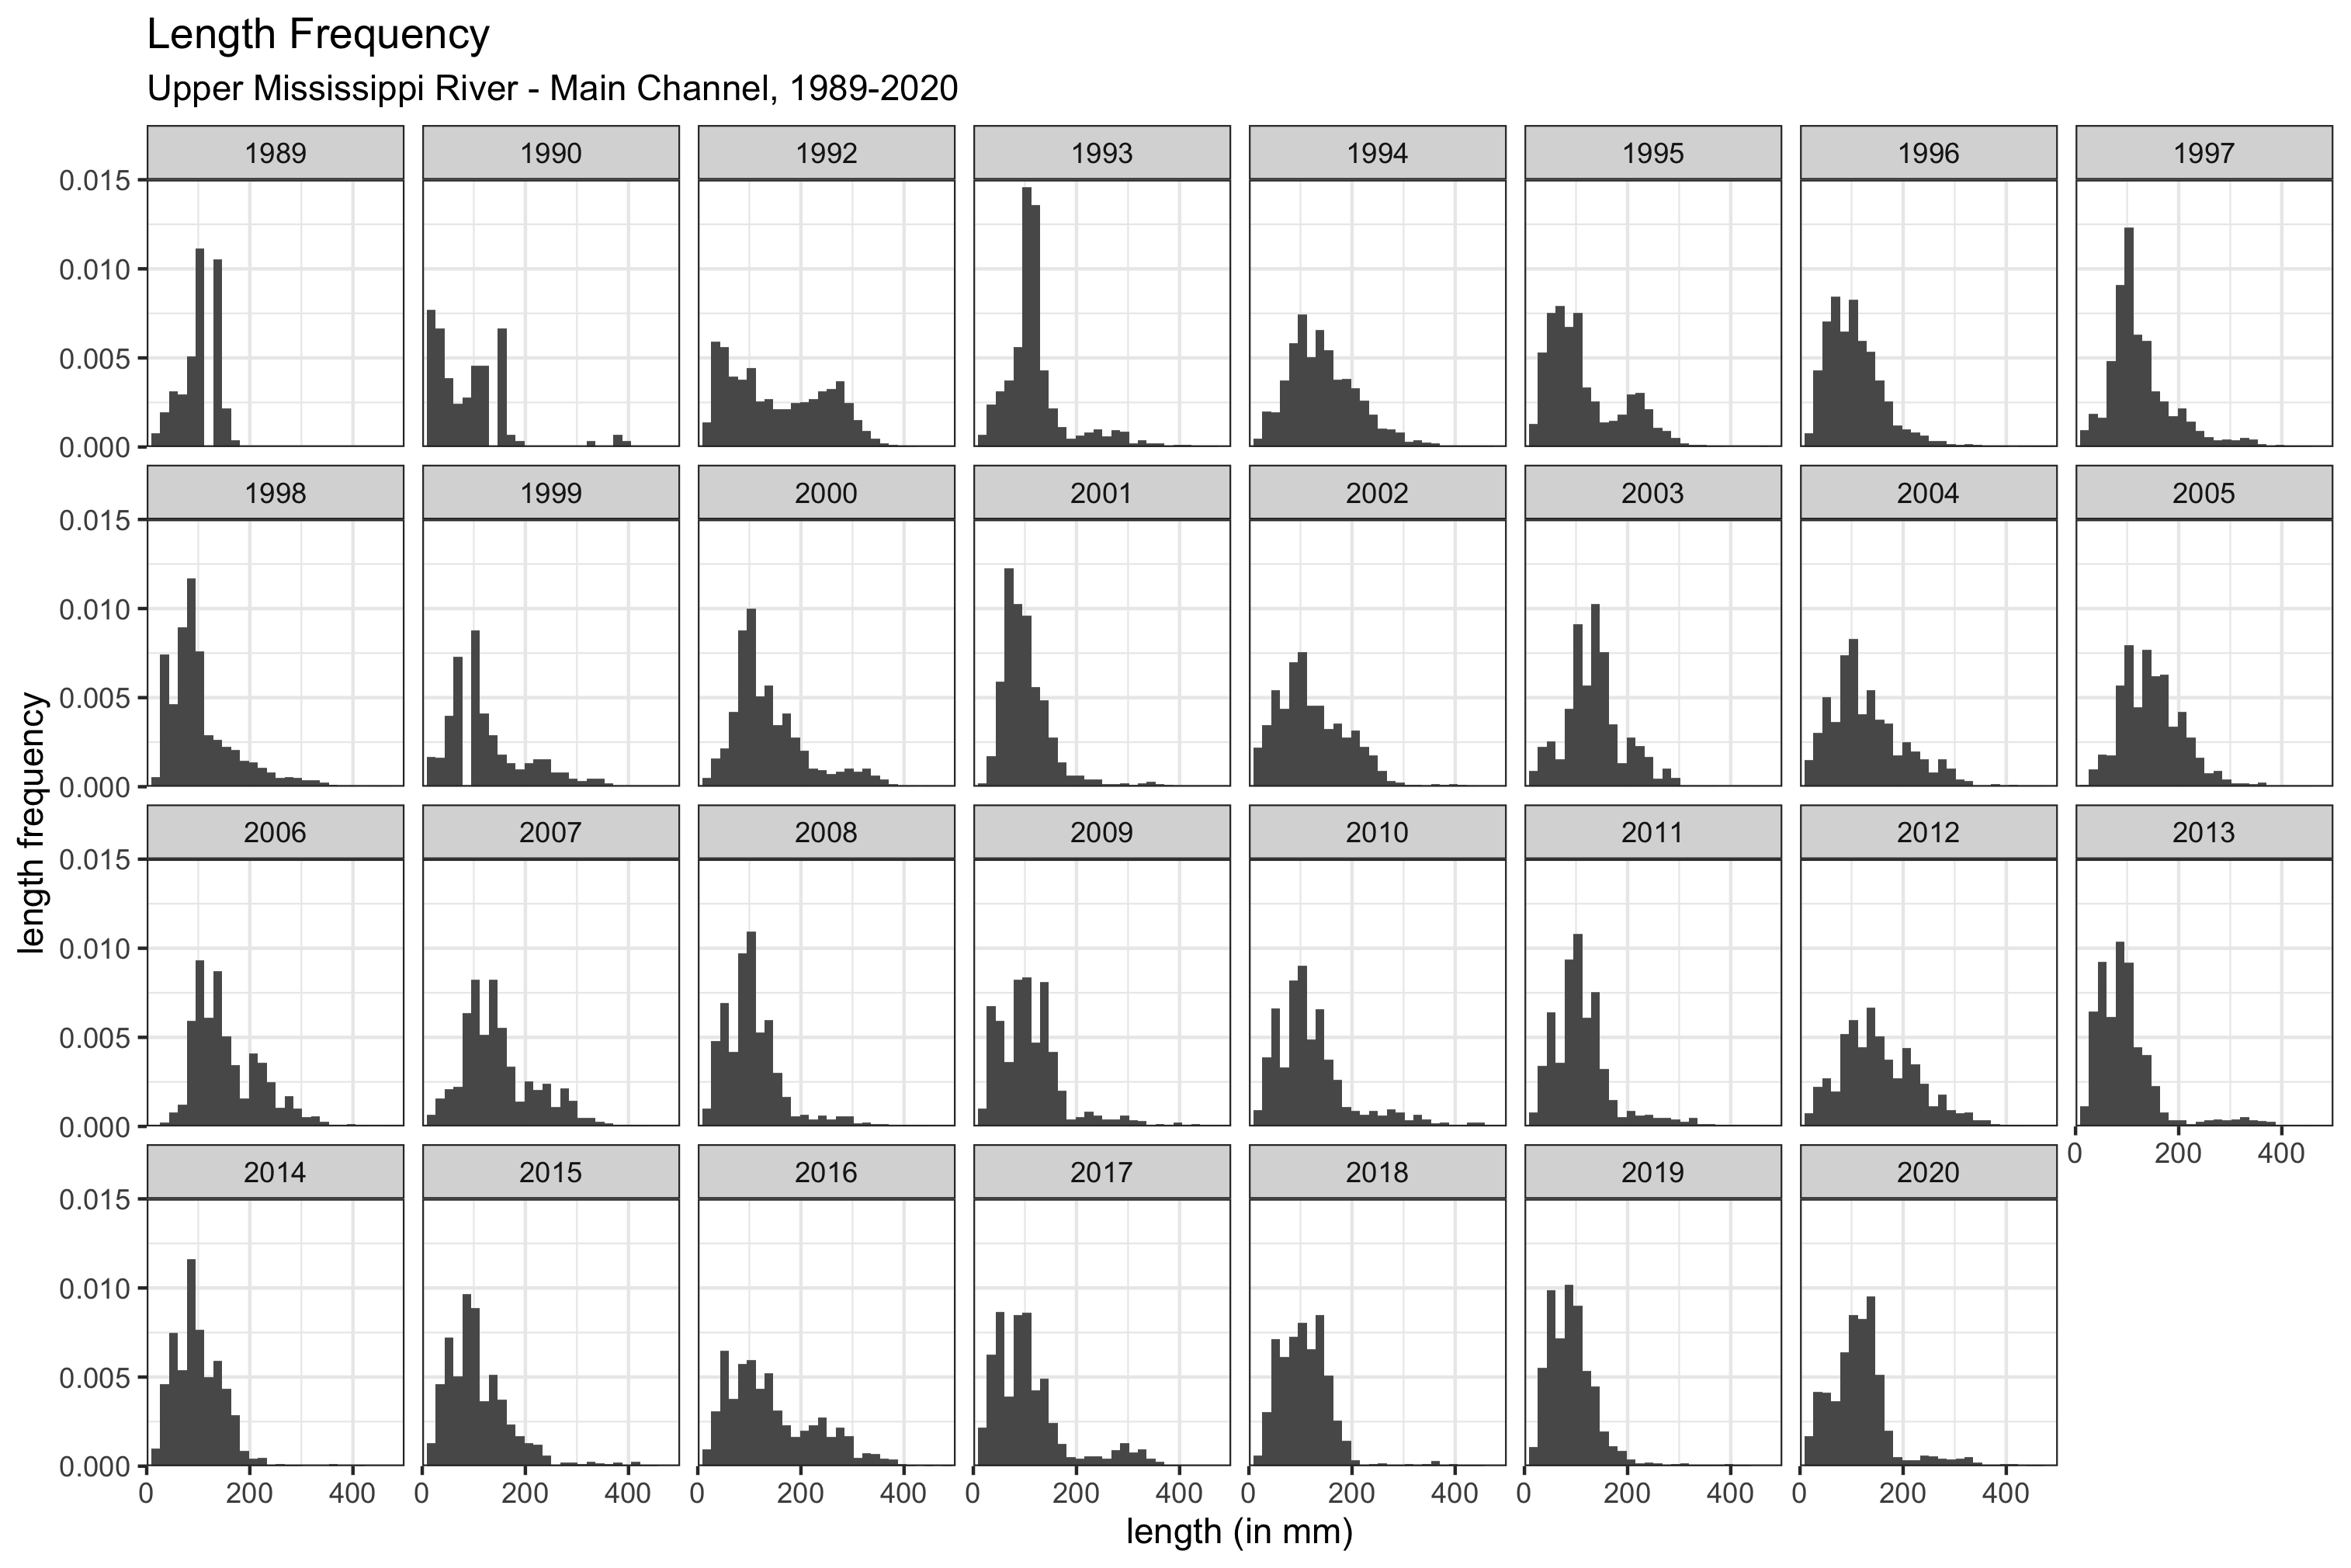
\includegraphics[width=1.2\textwidth]{figures/LTRMmain.png}
   \caption{}
   \label{fig:LTRMmain}
\end{subfigure}
\caption{(a) The LTRM fish survey sites in the Upper Mississippi River system. (b) Length frequency of sampled gizzard shad in the main channel of the Upper Mississippi River system.}
\end{figure}    

\subsubsection{Fecundity and recruitment}
Female gizzard shad begin reproducing at approximately 140 mm in length and egg numbers tend to increase with fish size \citep{jons1997ovarian}. 
The logistic parameters for the mean number of eggs produced by females of a certain length were obtained by fitting the three-parameter logistic function (Equation \ref{eq:egg}) to the data for batch fecundity versus length \citep{jons1997ovarian} (Figure \ref{fig:eggs}). 
Fish survival to age-1 was assumed to be dependent on the density of age-0 gizzard shad (Figure \ref{fig:surv_age0}).  
Parameters for the exponentially decaying age-0 survival function (Equation \ref{eq:s0}) were determined by fitting equation \ref{eq:s0} to the survival means for 2003-2007 cohorts of gizzard shard in five Missouri reservoirs \citep{michaletz2010overwinter}.
To complete the recruitment process we assign a length to the recruited individuals by simulating a Gaussian random variable with mean $\mu_c$ and standard deviation $\sigma_c$.
The parameters for the size distribution of age-1 fish were gleaned from a study of gizzard shad located in large impoundments \citep{michaletz2017variation} and the historic 1990-2020 LTRM dataset from the main channel of the UMRS (discussed in Section \ref{LTRM}).

\begin{figure}
\centering
\begin{subfigure}[b]{.43\textwidth}
  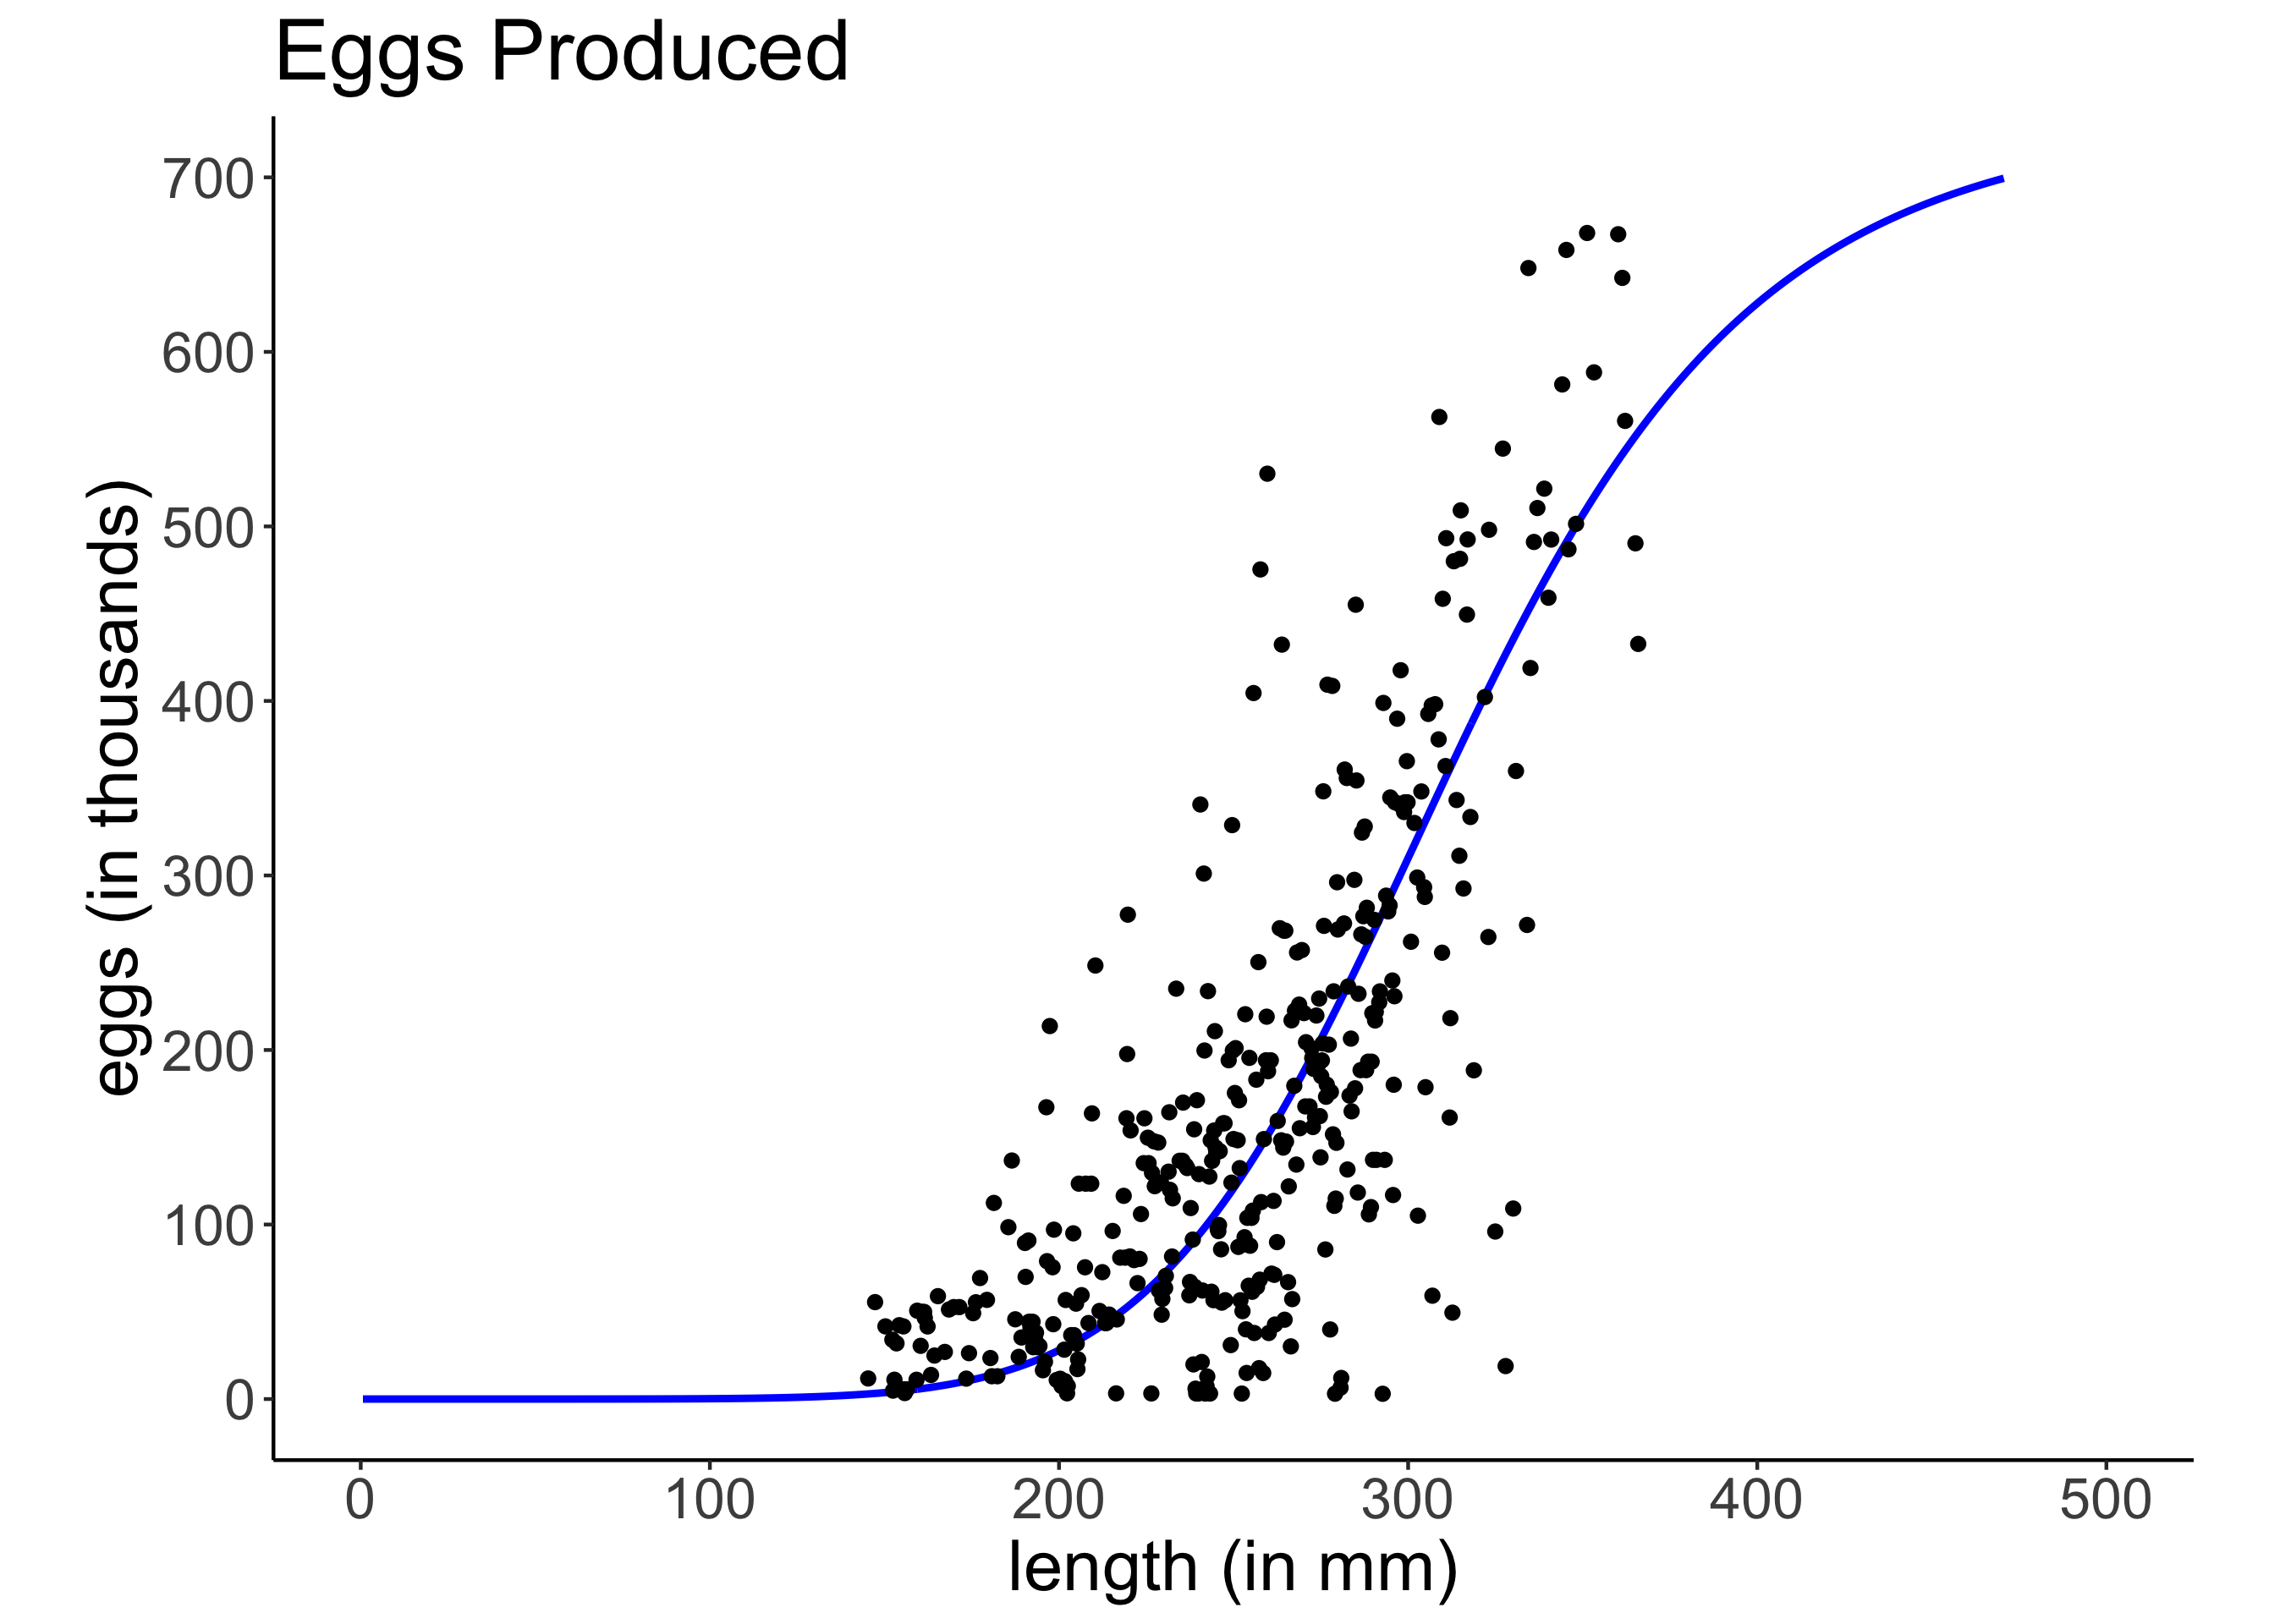
\includegraphics[width=\textwidth]{figures/eggs.png}
  \caption{}
  \label{fig:eggs}
\end{subfigure}
\begin{subfigure}[b]{.43\textwidth}
  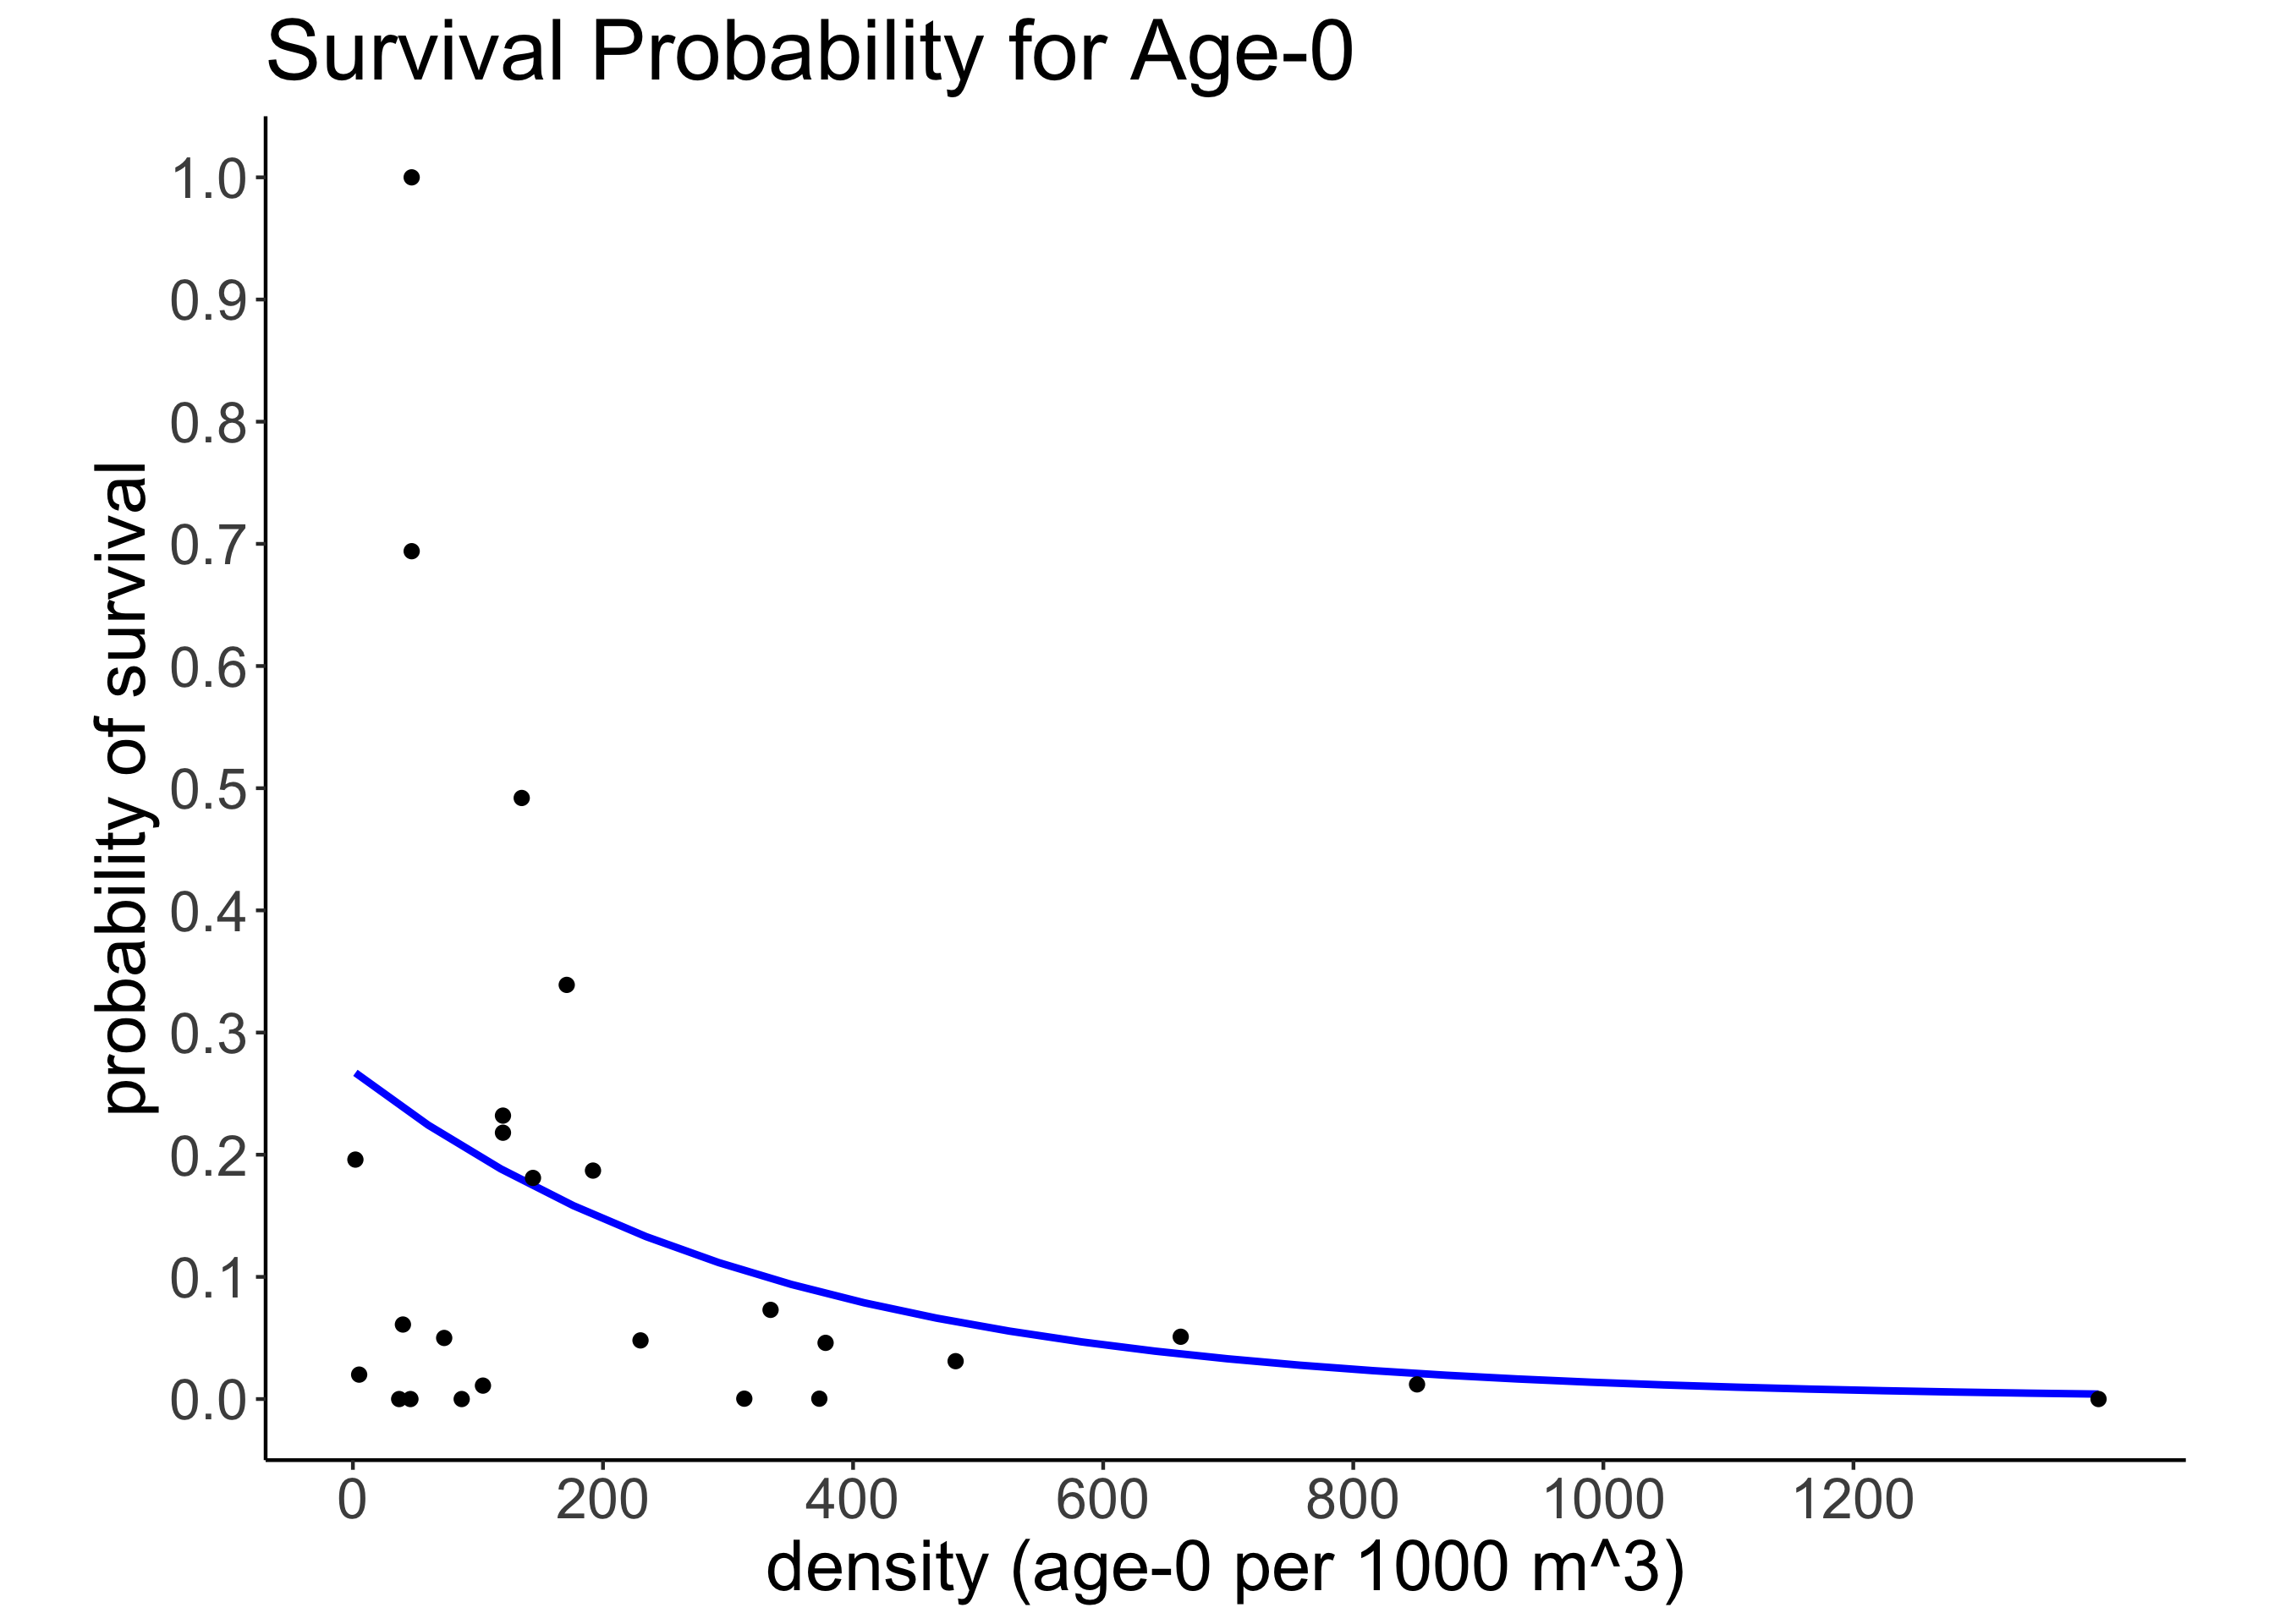
\includegraphics[width=\textwidth]{figures/age0surv.png}
  \caption{}
  \label{fig:surv_age0}
\end{subfigure}
\caption{(a) Mean number of eggs produced by female gizzard shad $\mbox{egg}(z)$. Data from \citep{jons1997ovarian}.  (b) Age-0 density-dependent survival function $s_0(d)$. Data from \citep{michaletz2010overwinter}. }
\label{fig:fecundity}
\end{figure}    

\subsubsection{Growth and survival of adults}
The parameters for the growth function were chosen as the mean values published on a study of gizzard shad located in large impoundments in Missouri U.S.A. \citep{michaletz2017variation}. 
The association between adult lengths and survival have not been well-resolved in gizzard shad leading us to make a number of assumptions.  
First, we assume that the probability of adult survival is related to the length by a four-parameter logistic function (Equation \ref{eq:surv}).
An investigation of gizzard shad in Lake Eerie \citep{bodola1955life} provided the minimum and maximum survival rate of adults. 
Based on the observed length distributions of gizzard shad sampled from the main channel of the Mississippi River (Figure \ref{fig:LTRMmain}), we assumed that solutions of our model will exhibit periodic behavior every 8-9 years.   
We used a least squares method to estimate the $\alpha_s$ and $\beta_s$ parameters that 
minimized the total square-distance between the (observed) pre-carp LTRM length distribution in the main channel of the UMRS and (predicted) model equilibrium, $n(z,t)$ during a 8-year period occurring 100 years after initialization.  
The slope parameter $\beta_s$ was found to be large in magnitude resulting in a primarily two-valued survival probability.  
Gizzard shad less than $\alpha_s$ mm in length have a very low survival rate ($\ds s_{\rm {min}}$) while lengths larger than  $\alpha_s$ mm approach the maximum survival rate $\ds s_{\rm {max}}$. 
This survival pattern has been reported for a number of fish species and can arise due to a number of biotic (i.e. predation) and/or abiotic (i.e. temperature) factors (Pepin et al., 1992; Nowlin et al., 2006). 
\section{Analysis and results}
We numerically solved the integral model using the Midpoint Rule with large approximating matrices \citep{burden2005numerical}. 
The Midpoint Rule has been commonly used for integral projection models because of its simplicity and effectiveness \citep{ellner2006integral, ramula2009integral,  merow2014advancing}. 
During the course of model development, we explored different step sizes for the Midpoint Rule and found that about 50 points provided numerically stable results. 
We integrated over lengths from 0 mm to 500 mm. 
The upper limit was chosen based upon numerical stability and consistency of the system (e.g., avoiding eviction or the loss of individuals due to numerical errors \citep{williams2012avoiding}). 

\subsection{Initial conditions}  We assumed that the initial density of gizzard shad was $d_0 = 964.7$, the annual average density of gizzard shad observed in La Grange Reach from 1993-2020.  
The probability of an individual being length $z$ at time $t=0$  was assumed to be normally distributed with mean $0.5L_\infty$ and standard deviation $\sigma_0 = 30$.  
As a result, we initialized our model with length distribution
\begin{equation}\label{eq:n}
 n(z,0) = d_0 \mbox{Norm} (0.5 L_\infty, \sigma_0) = 964.7 \mbox{Norm} (197.15, 30). 
 \end{equation}

The model was coded in R \citep{R} and the scripts are published on JP's GitHub page \verb+https://github.com/jppeirce+.

\subsubsection{Effect of density-dependence on the survival probability of the age-0 cohort} \label{sec:survival}

In the simulated solutions to the IPM, the density of age-0 Fish strongly influenced the density of gizzard shad at subsequent developmental stages.
When adult densities are large, there may be more fish of longer lengths that can produce a greater number of eggs.  
More eggs leads to a higher density of age-0 fish and reflectively a reduction in the survival to age-1. 
If reduced survival continues over subsequent years, the overall density of fish within the population may decline and result in a smaller number of longer length fish that are reproducing.  
Fewer fish spawning could result in a smaller age-0 class which, in turn, could enhance survival probability in this cohort (through reduced competition). 
We would then expect the overall density of fish to increase over the following years, until large numbers of eggs are again produced by larger, adult fish.  
This oscillatory pattern is reflected in our model by the time-dependent survival probability of age-0 recruits (Figure \ref{fig:age0time}).

\begin{figure}
\centering
  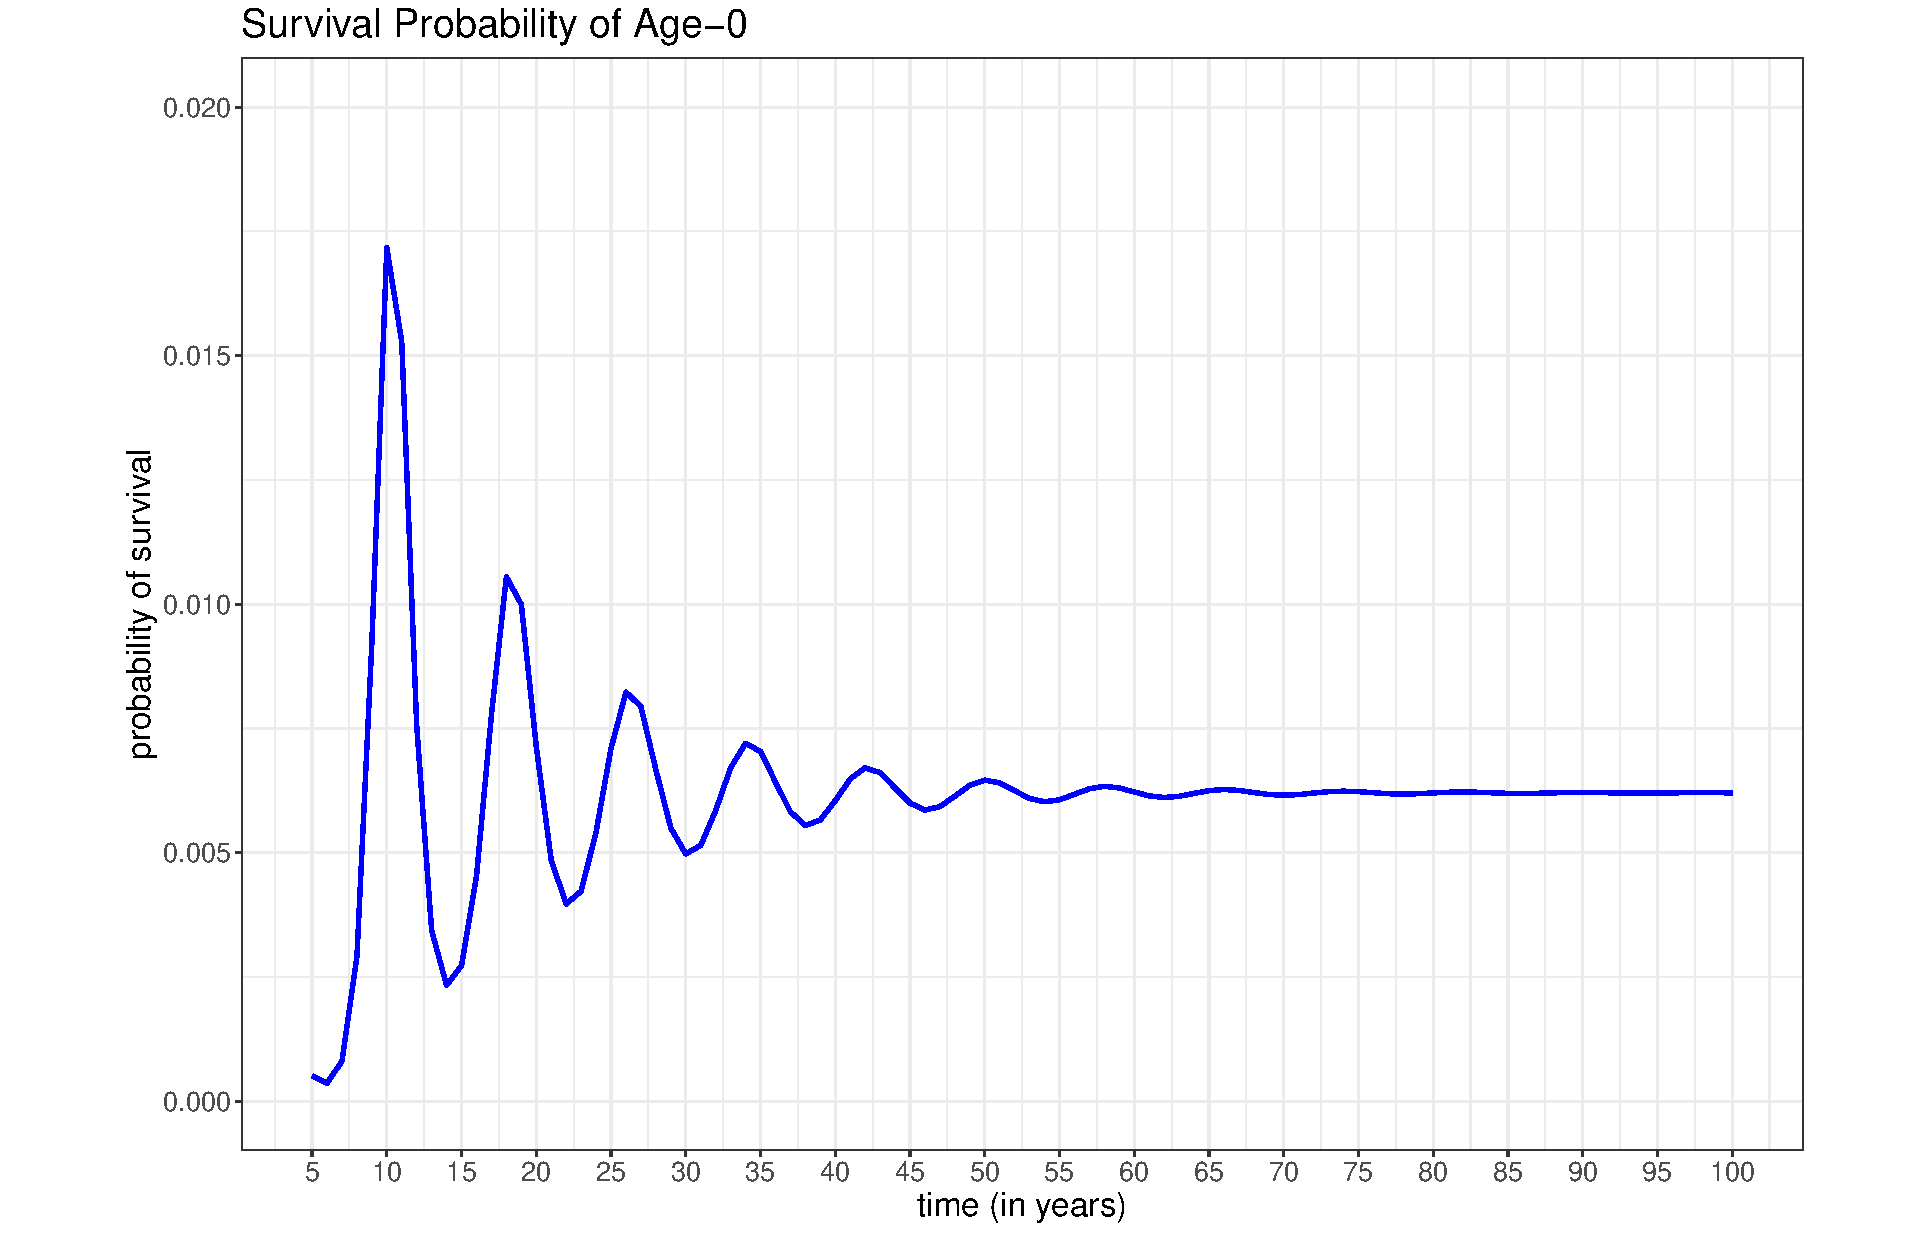
\includegraphics[width=.4\textwidth]{figures/Figure2a.pdf}
   \caption{}
  \label{fig:age0time}
 
\caption{Survival probability of age-0 gizzard shad.}

\end{figure}    

\subsubsection{Periodic orbit and validation with external dataset}
\begin{figure}
\centering
\begin{subfigure}[b]{.45\textwidth}
  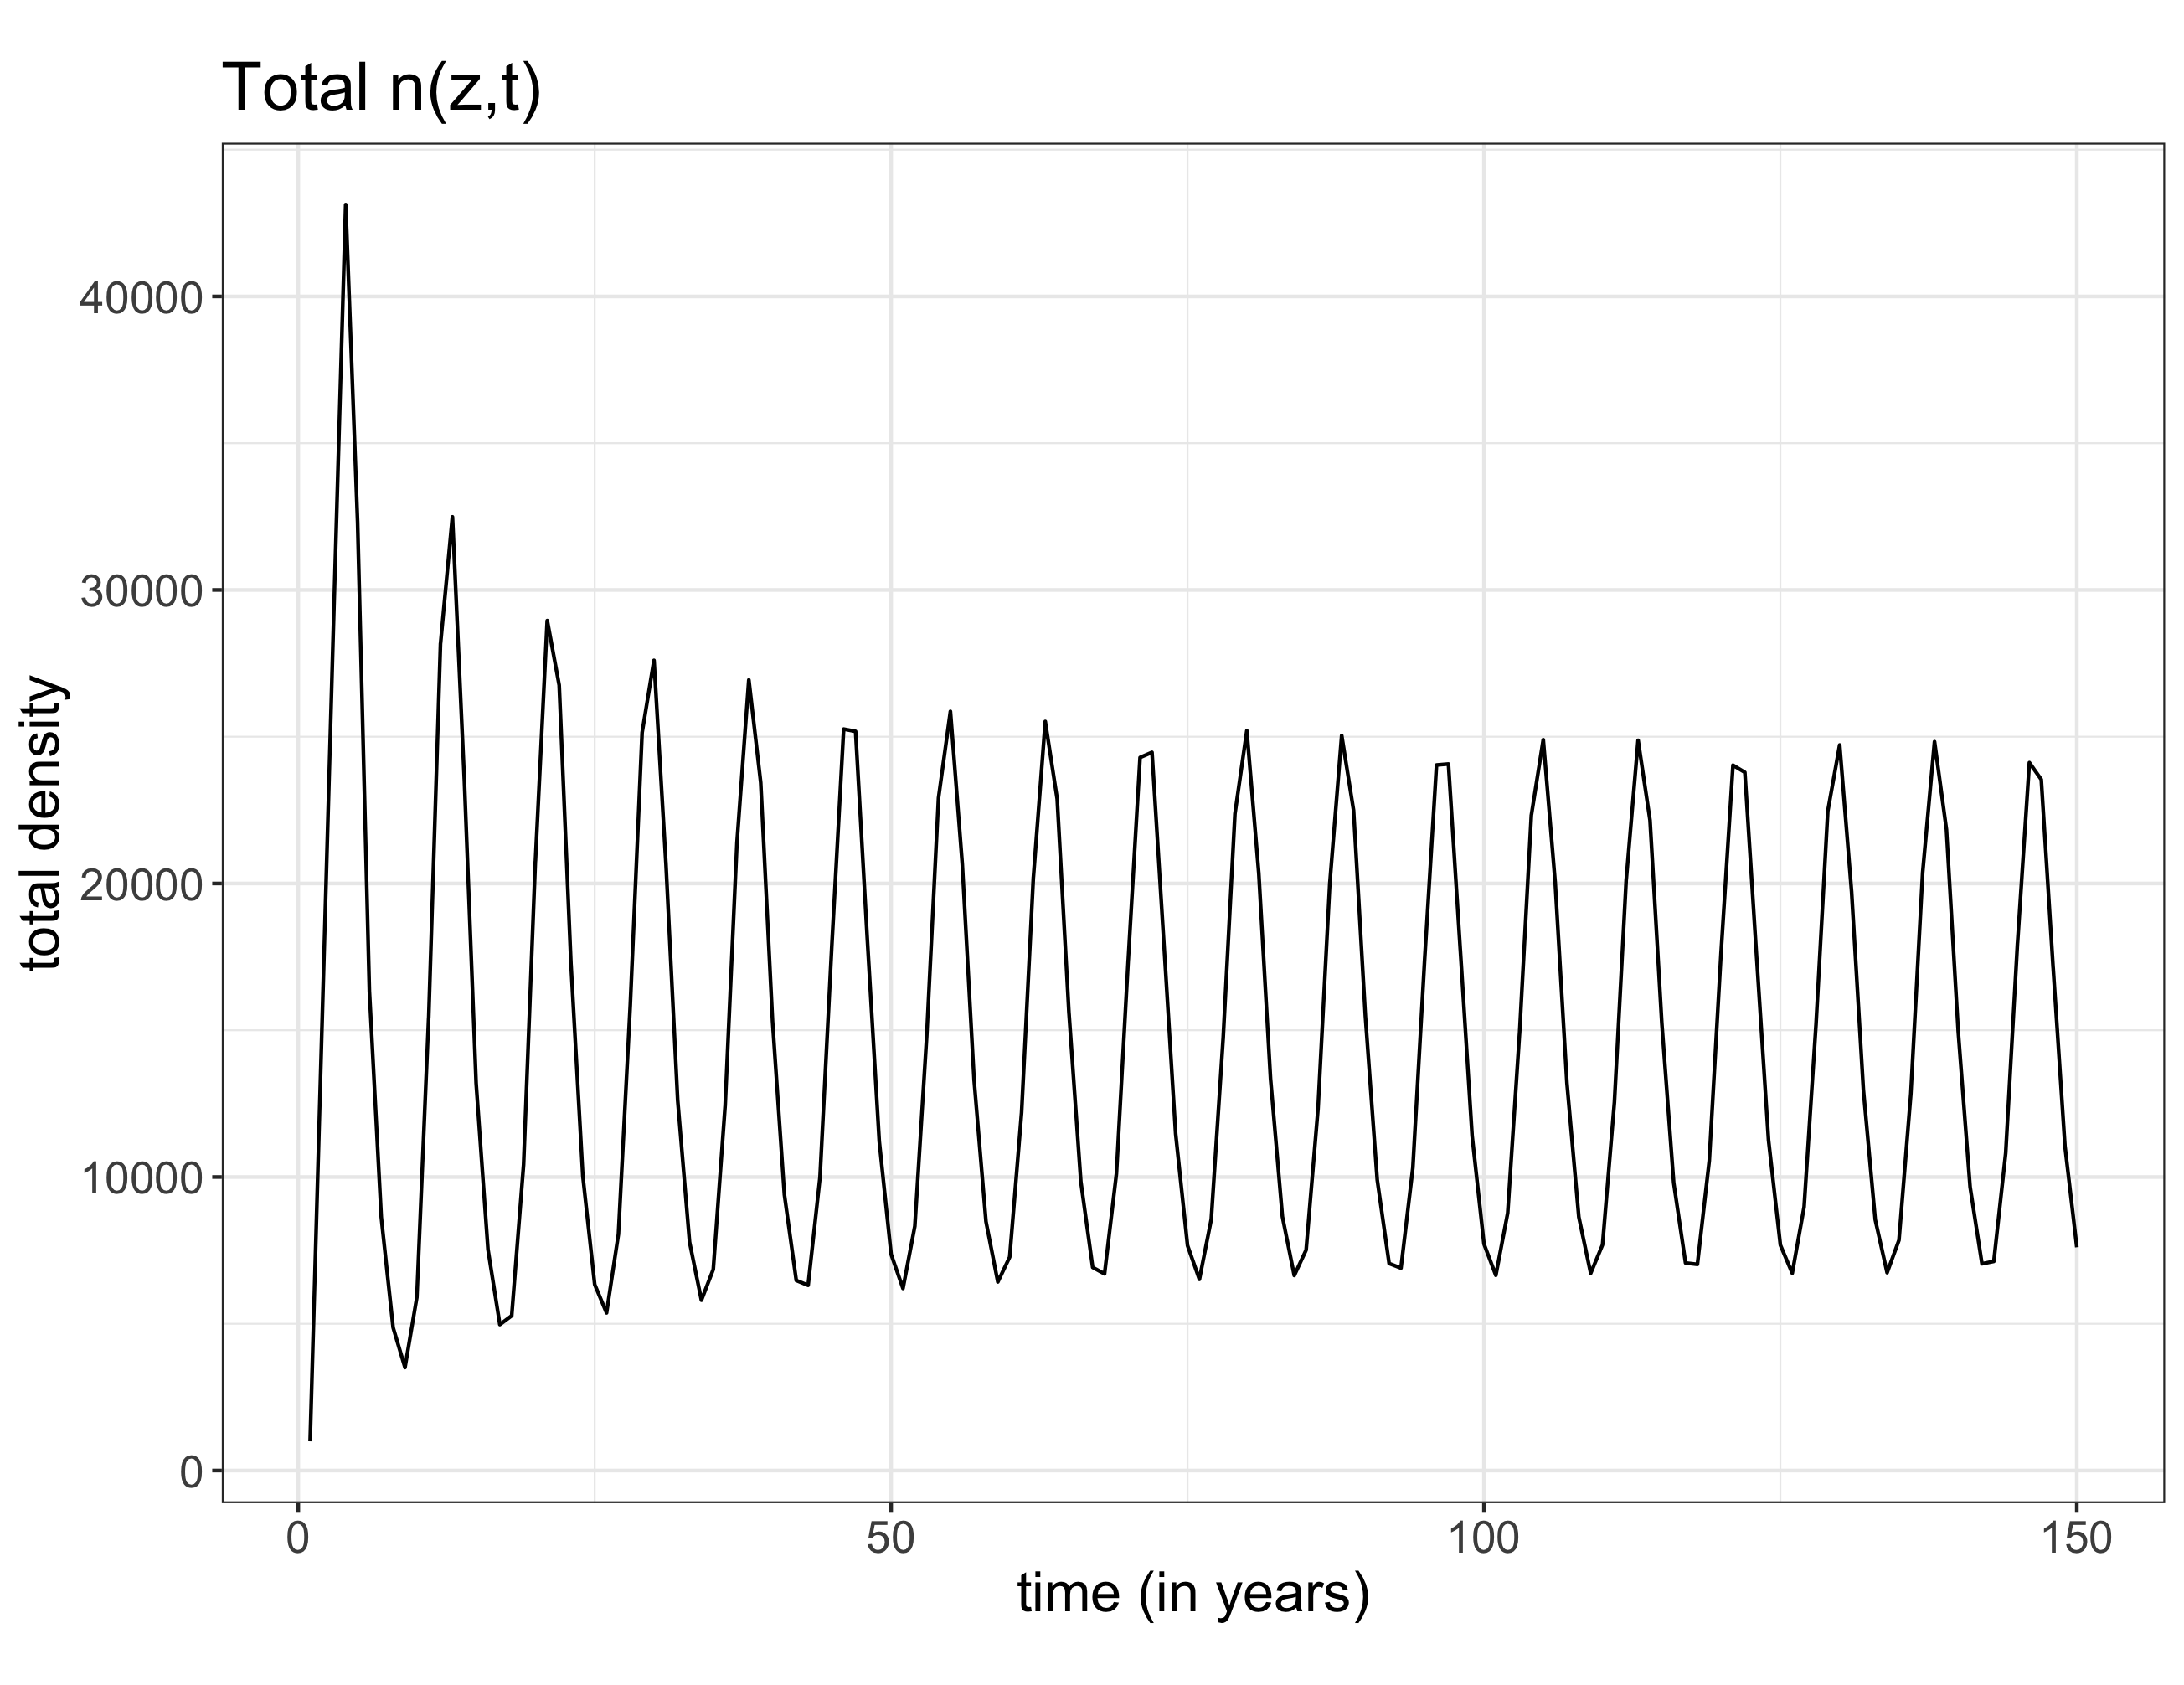
\includegraphics[width=\textwidth]{figures/ntotal.png}
   \caption{}
  \label{fig:ntotal}
\end{subfigure}
\begin{subfigure}[b]{.45\textwidth}
 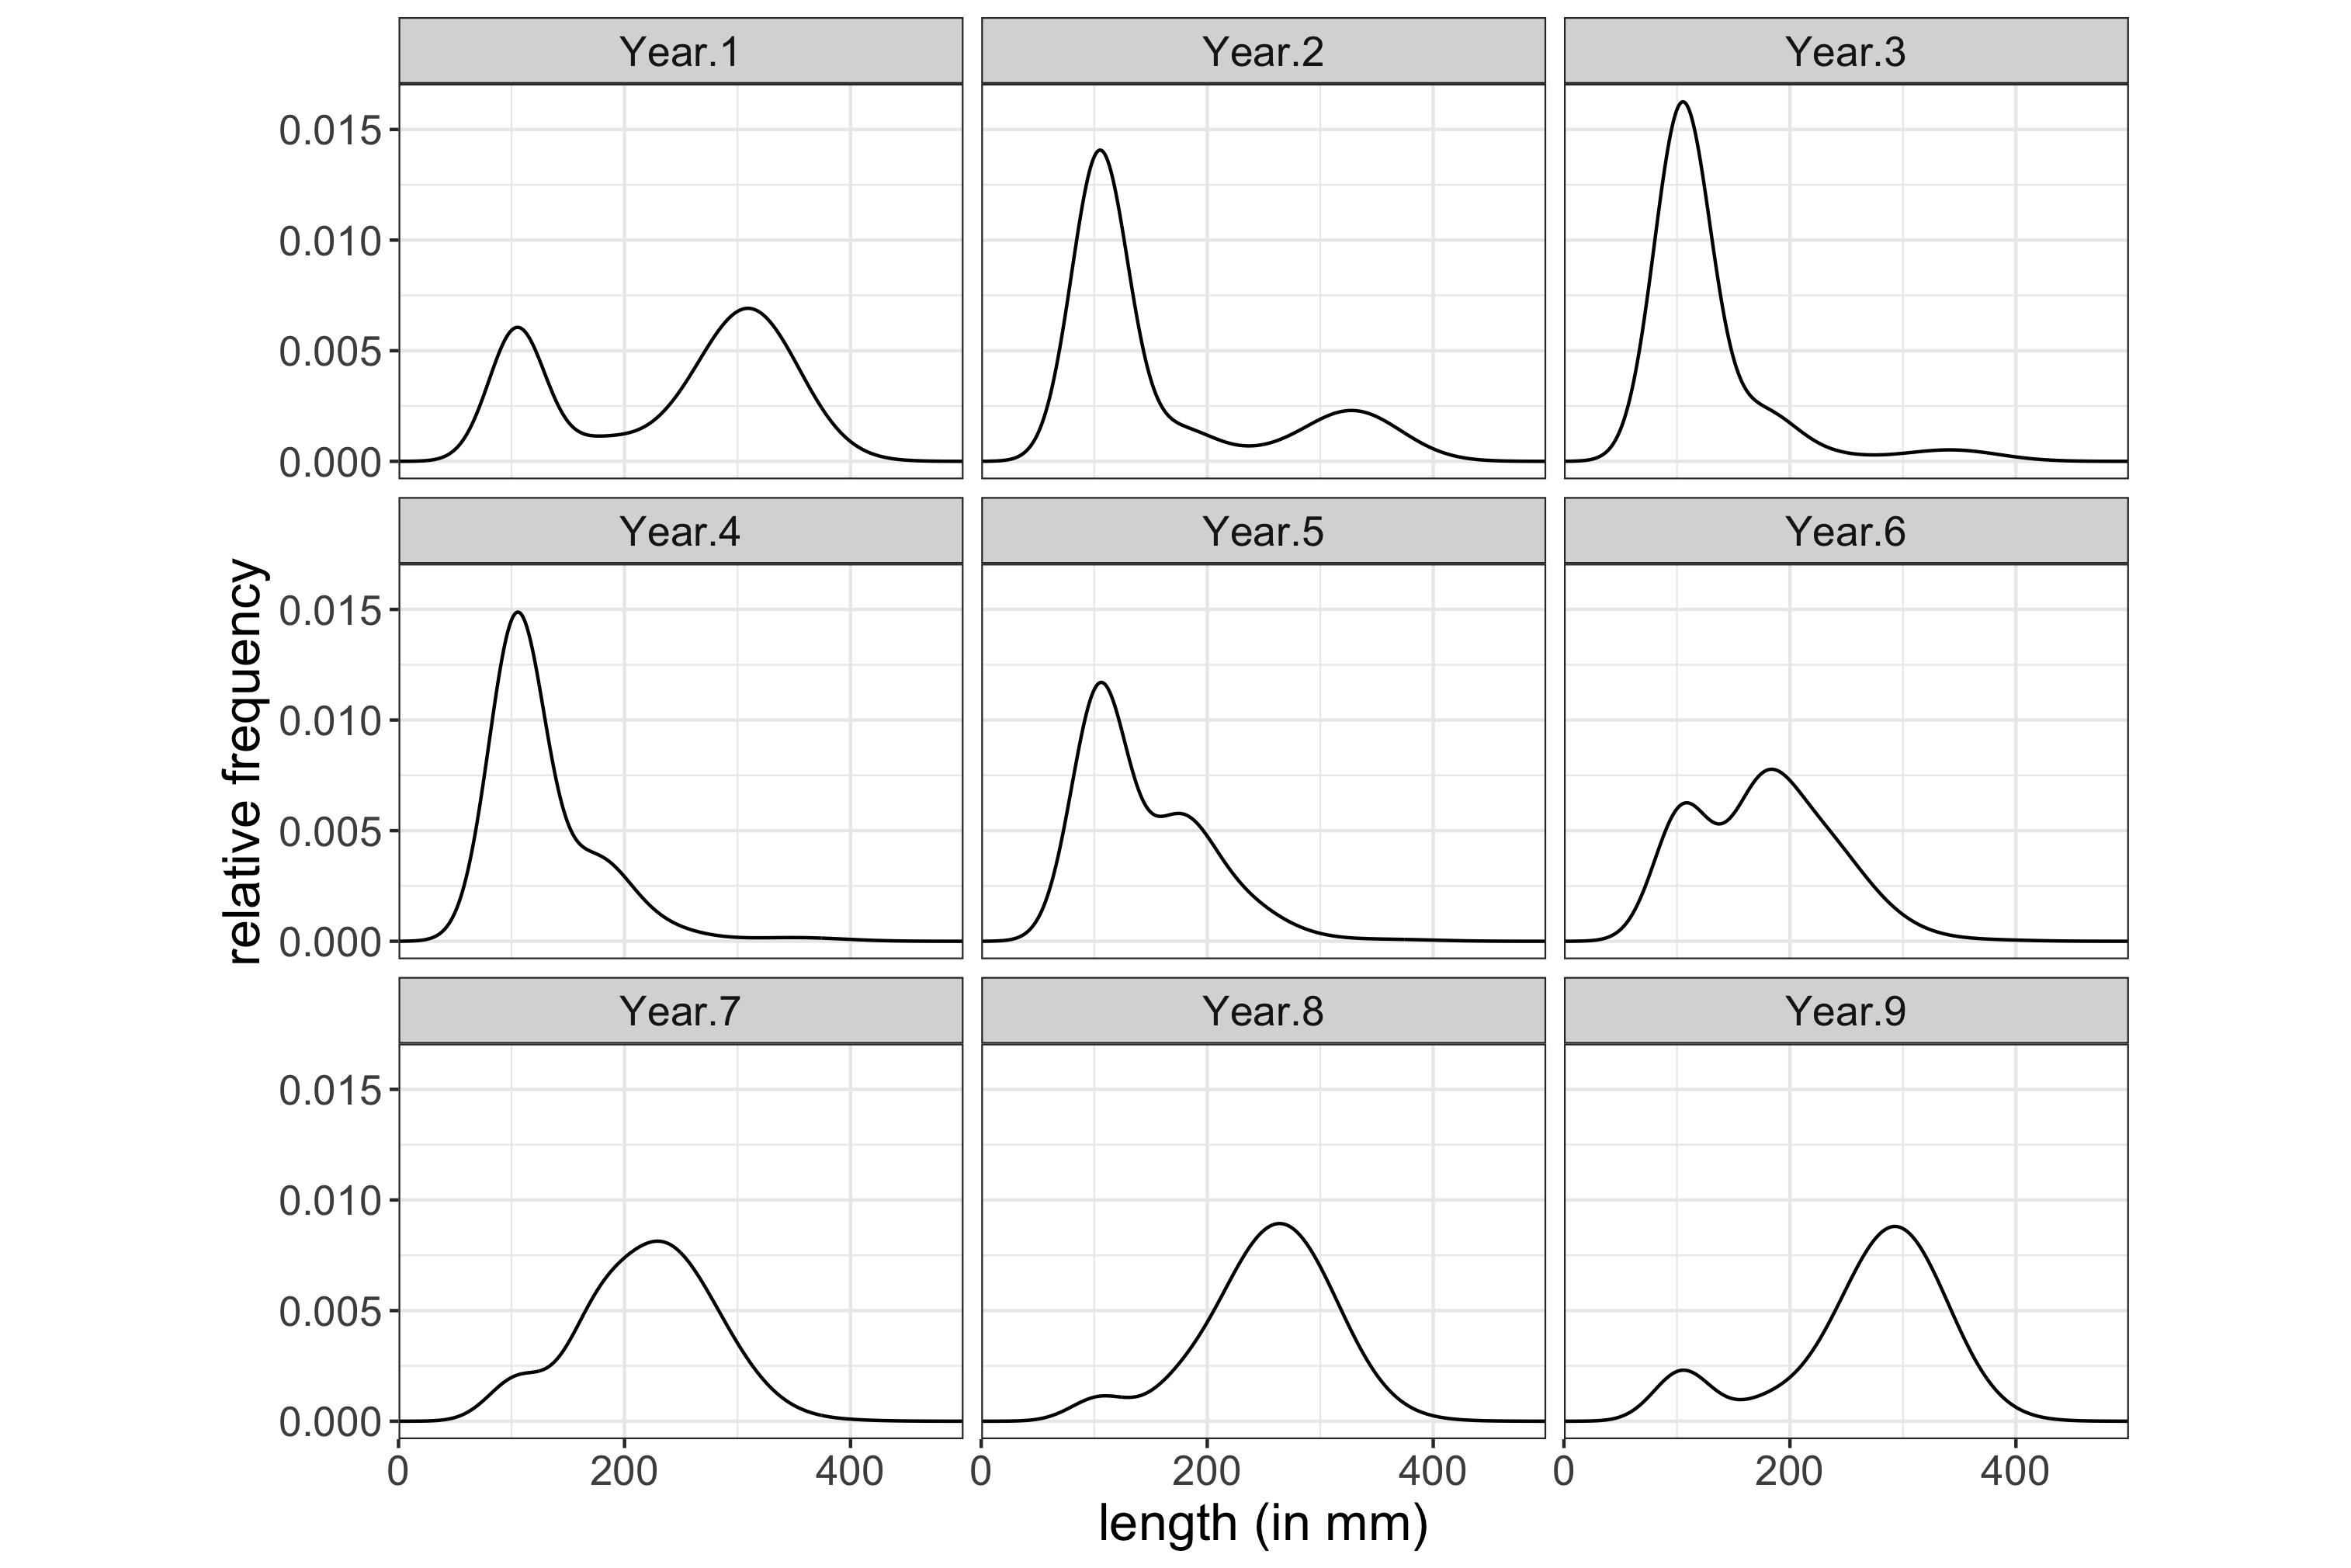
\includegraphics[width=\textwidth]{figures/period_facet.png}
     \caption{}
\label{fig:period}
\end{subfigure}
\caption{(a) The total density of gizzard shad in La Grange Reach predicted by the IPM in the first 100 years. (b) Simulated length distributions during a 9 year interval of time (approximately 1 period of the total density function).}
\end{figure}    

\begin{figure}
\centering
\begin{subfigure}[b]{.43\textwidth}
  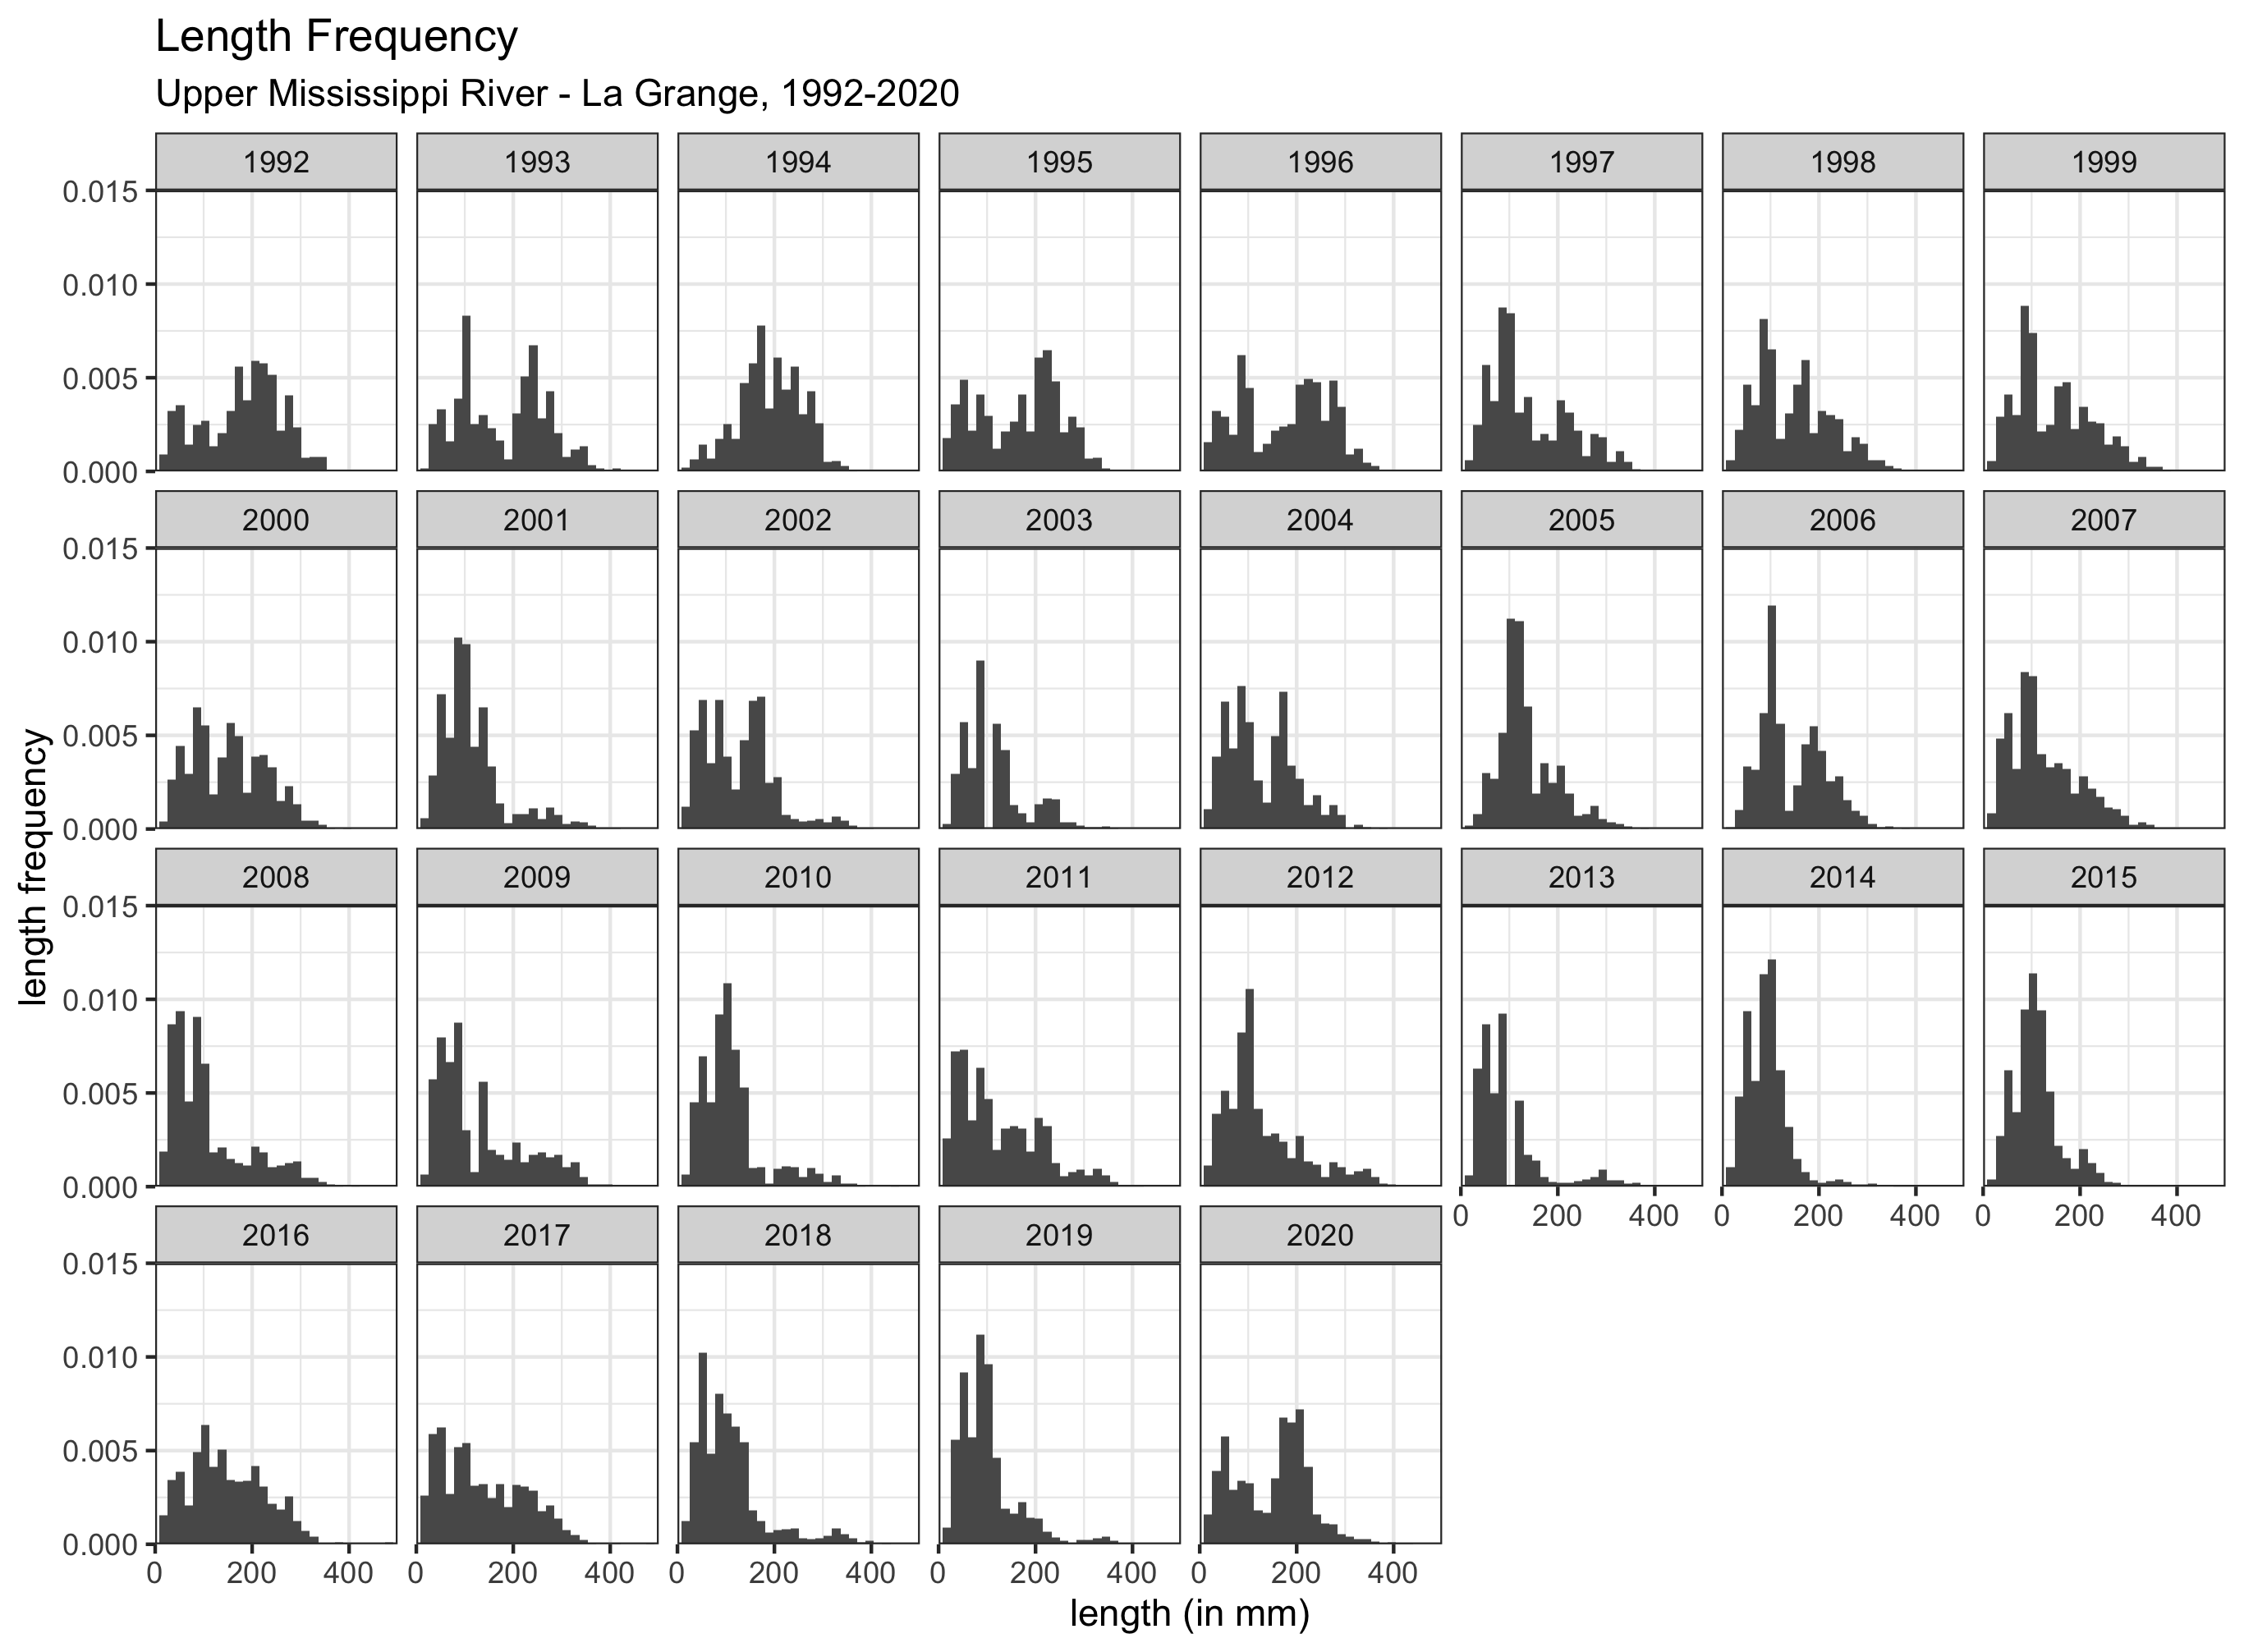
\includegraphics[width=\textwidth]{figures/LTRMlg.png}
   \caption{}
  \label{fig:LTRMlg}
\end{subfigure}
\begin{subfigure}[b]{.43\textwidth}
   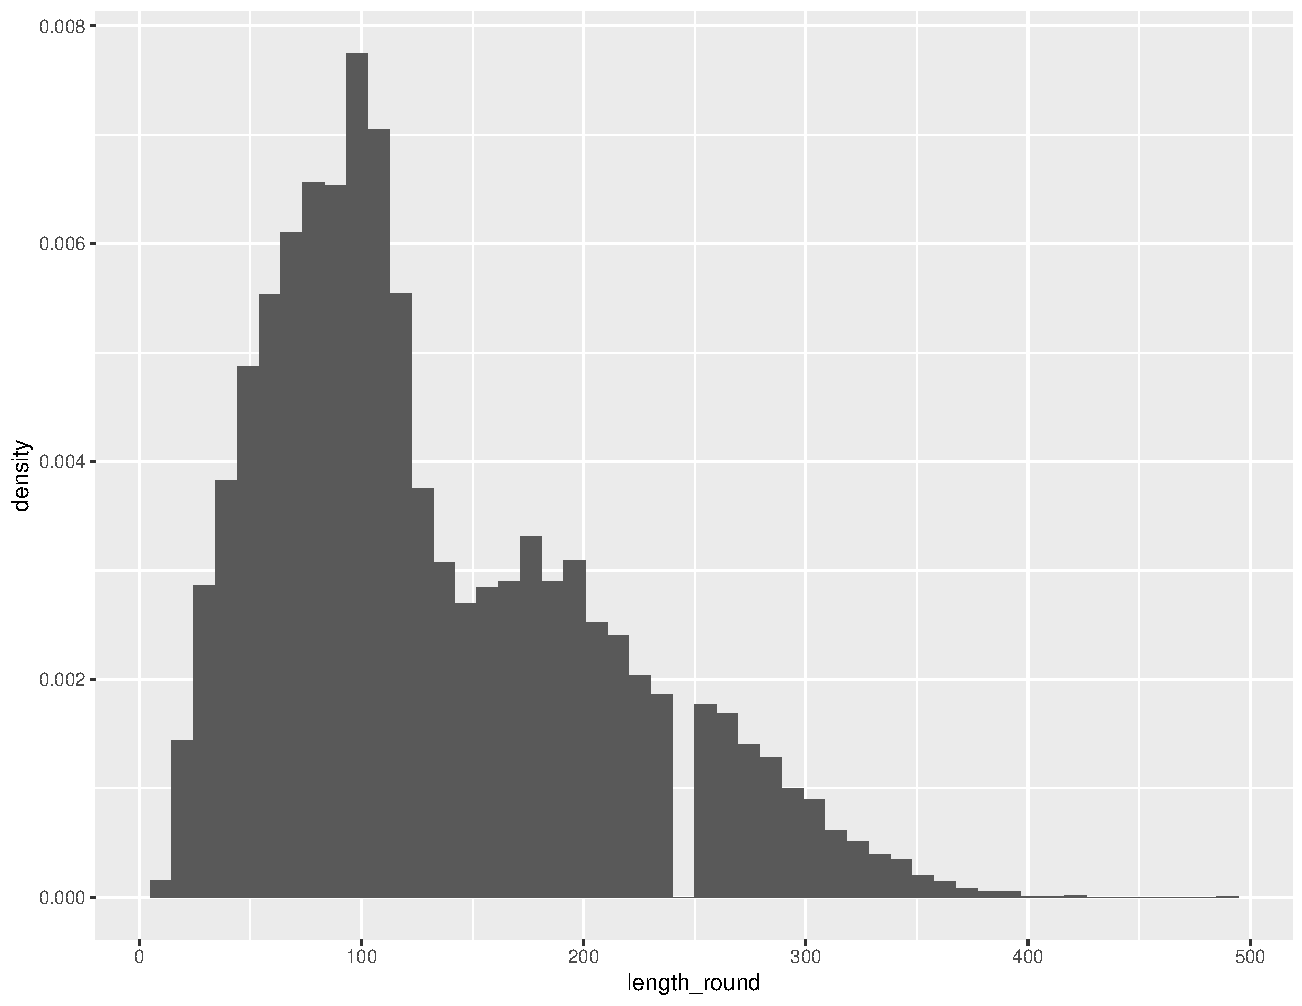
\includegraphics[width=\textwidth]{figures/lagrange.pdf}
     \caption{}
\label{fig:lagrange}
\end{subfigure}
\caption{(a) Length frequencies of sampled gizzard shad in La Grange for each year, 1992-2020. (b) Overall length frequencies of gizzard shad sampled in La Grange Reach from 1992-2020 compared with the average (over 1 period) simulated length frequency.}
\end{figure}    
The total number of gizzard shad in our simulation reached a stable periodic orbit (Figure \ref{fig:ntotal}) within 50 years. 
After simulating an additional 50 years, we fit a periodic function to the annual density of gizzard shad and determined the period of approximately 8.74 years. 
Figure \ref{fig:period} illustrates the periodic length dynamics within the gizzard shad population during a 9-year window of the periodic orbit.  
As a validation of the model, the simulated length distributions during a periodic orbit (Figure \ref{fig:period}) have similarities to fish lengths observed from the La Grange Reach (Figure \ref{fig:LTRMlg}). 
In addition, the ebb and flow of the frequency of the age-1 cohort can be observed and is associated with the density-dependent survival function for age-0 fish (explained in Section \ref{sec:survival}).

\section{Discussion}
Gizzard shad are common in freshwater systems of North America where they contribute to the integrity of aquatic communities. 
Given this, it is important to understand how populations of this species vary with changing environmental circumstances, such as the occurrence of invasive species. 
Herein, we use both LTRM data and parameters gleaned from other empirical studies to develop an integral projection model for gizzard shad and test model outputs against patterns reported from a well-studied population of this species from the La Grange Reach of the Illinois River.   

After fitting two adult survival parameters using LTRM data from the main channel of the Mississippi River, we compared a simulated length distribution with empirical data collected from the La Grange Reach of the Illinois River from 1992 to 2020. 
The resulting simulated length distributions (Figure \ref{fig:period}) reflected a number of the patterns observed in gizzard shad captured from the La Grange Reach over the same timeframe (Figure \ref{fig:LTRMlg}). For example, the predicted transition from bimodal length distributions to a single peak in smaller gizzard shad in our simulations was reflected in the empirical data from  1996 to 2000.  This trend was also observed from 2004-2008.  It should be noted, that there were also discrepancies between model simulations and the empirical data.  In particular, we did not notice a distinct, single peak in intermediate sized fish in field collections even though this was predicted by our model. Temporal and spatial variation in environmental parameters of the La Grange Reach and their impacts on the gizzard shad population may explain why certain trends from the field were not well represented in our IPM outputs.   

The average (over 1 period) simulated length frequency compares well with the overall length frequencies of  gizzard shad sampled in La Grange Reach from 1992-2020 (Figure \ref{fig:lagrange}). 
Peak frequencies are near the same lengths with the model predicting slightly higher density of adult lengths and fewer juvenile lengths than observations. 
This may be explained by gear type and capture method which vary from site to site potentially introducing bias in the observed length distributions year to year.
In addition, studies also suggest that environmental stochasticity and food variability may alter recruitment densities which are difficult to measure accurately \citep{rose2000quantitative, okamoto2016stochastic}. 

While our model uses the density of age-0 gizzard shad to affect the survival probability in their first year, we assumed constant viability which may be sensitive to the external factors mentioned above.
In addition, the location of the maximum length and the variation in the of length of new recruits recorded in the LTRM data, suggests that there may be smaller age-0 fish in La Grange Reach than in the study location \citep{michaletz2017variation} used to parameterize the model.  

Gaining an understanding of how length distributions of gizzard shad emerge under density-dependent survival in the age-0 class will serve as a foundation for investigating density effects at subsequent stages in the life cycle.  
In addition, this single-species model could also be expanded to incorporate interspecific interactions between gizzard shad and species such as invasive carp, which appear to negatively impact gizzard shad life-histories through competition for food resources.   

\section{Acknowledgments}

These data are a product of the U.S. Army Corps of Engineer's Upper Mississippi River Restoration Program (UMRR) Long Term Resource Monitoring (LTRM) element implemented by the U.S. Geological Survey in collaboration with the five Upper Mississippi River System (UMRS) states of Illinois, Iowa, Minnesota, Missouri, and Wisconsin.
The U.S. Army Corps of Engineers (Corps) provides guidance and has overall program responsibility.

We thank the U.S.~Geological Survey  Biological Threats and Invasive Species Program and Great Lakes Restoration Initiative for funding.
In addition, research was supported by NSF-DMS Grant \#1852224, ``REU Site: Ecological Modeling of the Mississippi River Basin''. Any use of trade, firm, or product names is for descriptive purposes only and does not imply endorsement by the U.S. Government.

 \bibliographystyle{elsarticle-num-names} 
 \bibliography{gizshad}

\end{document}

\endinput
%%
%% End of file `elsarticle-template-num-names.tex'.
